% This must be in the first 5 lines to tell arXiv to use pdfLaTeX, which is strongly recommended.
\pdfoutput=1
% In particular, the hyperref package requires pdfLaTeX in order to break URLs across lines.

\documentclass[11pt]{article}

% Remove the "review" option to generate the final version.
\usepackage[review]{ACL2023}

% Standard package includes
\usepackage{times}
\usepackage{latexsym}
\usepackage{amsmath}

% Emojiis
\usepackage{emoji}

% For proper rendering and hyphenation of words containing Latin characters (including in bib files)
\usepackage[T1]{fontenc}
% For Vietnamese charactershttps://www.overleaf.com/project/6546c8a52c26a3b6897c971d
% \usepackage[T5]{fontenc}
% See https://www.latex-project.org/help/documentation/encguide.pdf for other character sets

% This assumes your files are encoded as UTF8
\usepackage[utf8]{inputenc}

% This is not strictly necessary, and may be commented out.
% However, it will improve the layout of the manuscript,
% and will typically save some space.
\usepackage{microtype}

% This is also not strictly necessary, and may be commented out.
% However, it will improve the aesthetics of text in
% the typewriter font.
\usepackage{inconsolata}

\usepackage{pdfpages}

\usepackage{csquotes}

\usepackage{listings}
\lstset{
  basicstyle=\ttfamily,
  breaklines=true,
}

\usepackage{multirow}

\usepackage{pifont}
\usepackage{xcolor}
\newcommand{\cmark}{\textcolor{green!80!black}{\ding{51}}}
\newcommand{\xmark}{\textcolor{red}{\ding{55}}}

\usepackage{makecell}

\usepackage{float}

\usepackage{colortbl}

\usepackage{graphicx}

\usepackage{enumitem} % Include this package

\usepackage{booktabs} % For formal tables
\usepackage{siunitx} % For aligning numbers by decimal point


% If the title and author information does not fit in the area allocated, uncomment the following
%
%\setlength\titlebox{<dim>}
%
% and set <dim> to something 5cm or larger.

\usepackage{ifthen}
 \newboolean{showcomments}
 \setboolean{showcomments}{true} % Set to false to hide all comments
\newcommand{\ryan}[1]{\ifthenelse{\boolean{showcomments}}{\textcolor{orange}{[#1 —ryan]}}{}}
\newcommand{\ananjan}[1]{\ifthenelse{\boolean{showcomments}}{\textcolor{green}{[#1 —ananjan]}}{}}
\newcommand{\will}[1]{\ifthenelse{\boolean{showcomments}}{\textcolor{pink}{[#1 —will]}}{}}
\newcommand{\cheng}[1]{\ifthenelse{\boolean{showcomments}}{\textcolor{purple}{[#1 —cheng]}}{}}
\newcommand{\emma}[1]{\ifthenelse{\boolean{showcomments}}{\textcolor{red}{[#1 —emma]}}{}}
\newcommand{\diyi}[1]{\ifthenelse{\boolean{showcomments}}{\textcolor{blue}{[#1 —diyi]}}{}}


% \title{Roleplay-doh: Enabling Peer Counseling Experts to Make and Shape LLM-Practice Partners for Conversational Roleplay}
\title{Roleplay-doh: Enabling Counseling Experts to Shape Roleplay Agents for Simulation Training}
% \title{Humans Learning From Large Language Model Feedback\\ Providing Tailored AI-Generated Feedback To Novice Helpers}

% Author information can be set in various styles:
% For several authors from the same institution:
% \author{Author 1 \and ... \and Author n \\
%         Address line \\ ... \\ Address line}
% if the names do not fit well on one line use
%         Author 1 \\ {\bf Author 2} \\ ... \\ {\bf Author n} \\
% For authors from different institutions:
% \author{Author 1 \\ Address line \\  ... \\ Address line
%         \And  ... \And
%         Author n \\ Address line \\ ... \\ Address line}
% To start a seperate ``row'' of authors use \AND, as in
% \author{Author 1 \\ Address line \\  ... \\ Address line
%         \AND
%         Author 2 \\ Address line \\ ... \\ Address line \And
%         Author 3 \\ Address line \\ ... \\ Address line}

\author{First Author \\
  Affiliation / Address line 1 \\
  Affiliation / Address line 2 \\
  Affiliation / Address line 3 \\
  \texttt{email@domain} \\\And
  Second Author \\
  Affiliation / Address line 1 \\
  Affiliation / Address line 2 \\
  Affiliation / Address line 3 \\
  \texttt{email@domain} \\}

\begin{document}
\maketitle
\begin{abstract}
Training novice counselors effectively requires realistic practice environments. Traditional use of role-play or standardized patients—trained actors—is often impractical due to high costs and limited availability. This work explores how to create virtual patients via large language models (LLMs) as an accessible alternative.
Instead of direct prompting that often results in non-authentic behaviors, 
% However, direct prompting of LLMs frequently results in non-authentic behaviors. B
we introduce a rapid co-design process that refines LLM-based virtual patients' behaviors to more accurately reflect patient interactions, by incorporating qualitative feedback from experienced counselors. Our approach demonstrates a practical method to enhance the realism of virtual patients, leveraging expert insights to improve counselor training.
\end{abstract}

\section{Introduction}


Realistic practice and personalized feedback are key for novice counselors to effectively learn clinical skills~\cite{nurse2024influence}.
% \diyi{add citation}
Simulation-based education methods, such as roleplay with peers or Standardized Patients~\cite{gliva2020comprehensive} and simulations with digital patients, can offer interactive practice opportunities that complement theoretical knowledge~\cite{kuhne2020standardized}.  
% \diyi{standardized patients could refer to role play and also "digital patients" that were created using earlier digital technologies.. here, are we only using it to refer to role play?}. 
However, each method has its limitations: practicing with peers is only viable if peers are experienced with the roleplay topic; Standardized Patients are used mostly for evaluation rather than practice due to the cost and availability of trained, human actors; and most digital patients operate using tailored, dialogue trees~\cite{othlinghaus2020seriousroleplaying}, which limits the diversity of dialogue scenarios that can be practiced.
% \diyi{could we elaborate it in a sentence or two? in addition to cost, avaiability, the diverse scenarios represented by these roleplay settings or tailored patients design are also issues? } 
Without appropriate practice opportunities, counselors may be underprepared or lack confidence for giving effective counseling support to real help-seekers. 
Therefore, innovating beyond traditional methods by developing versatile, AI-powered simulation tools could revolutionize the training landscape for counselors, making practice opportunities more varied and readily available~\citep{yang2024social}.
% \diyi{this paragraph is much better! to help us better respond to R2, i think it would be great to explicitly point out that both "practice" and "feedback" are important for helping novice counselors, and our current work only deals with "practice" side. }
% \diyi{standardized patients concept exist for a long time, even before LLMs. we should justify for why LLM based virtual patient is needed. Then among existing efforts to build LLM based virtual patients, why they are not enough? Then it would motivate our work of co-designing + principles ...} \ryan{I tried to lead with Standardized Ps and need for Virtual Ps}



Recent studies have explored the use of large language models (LLMs) to create virtual patients %  that could be used as dialogue partners for interactive practice of counseling and psychotherapy skills
~\citep{tanana2019development, demasi-etal-2020-multi, chen2023llmempowered}. While past methods fine-tuned models to clone multiple persona~\cite{demasi-etal-2020-multi}, this approach cannot create custom personas beyond what is in a dataset and can be limited when data is difficult to obtain due to privacy concerns. More recent techniques involve directly prompting LLMs to emulate a patient persona~\cite{chiu2024computational, tu2024conversational}. However, these simulations often fail to capture realistic patient behaviors (e.g., use colloquial language, show resistance to help) when evaluated by experienced therapists~\cite{chen2023llmempowered}. 
% \diyi{use a few example keywords to clarify "authentic"---what this means?} 
Thus, incorporating counselor feedback is essential for enhancing the realism of these simulations. Current methods for aligning models to human feedback involve collecting extensive preference data from experts for model re-training~\cite{christiano2017deep, rafailov2024direct} which is costly and time-consuming. % \ryan{Should I add back qualitative feedback, and system-designer in loop point?} 
In the mental health setting, there is a need for more efficient methods that allow therapists to provide information-rich, qualitative feedback to refine LLM simulations to better mimic realistic patient behavior. 

\begin{figure*}[t]
    \centering
    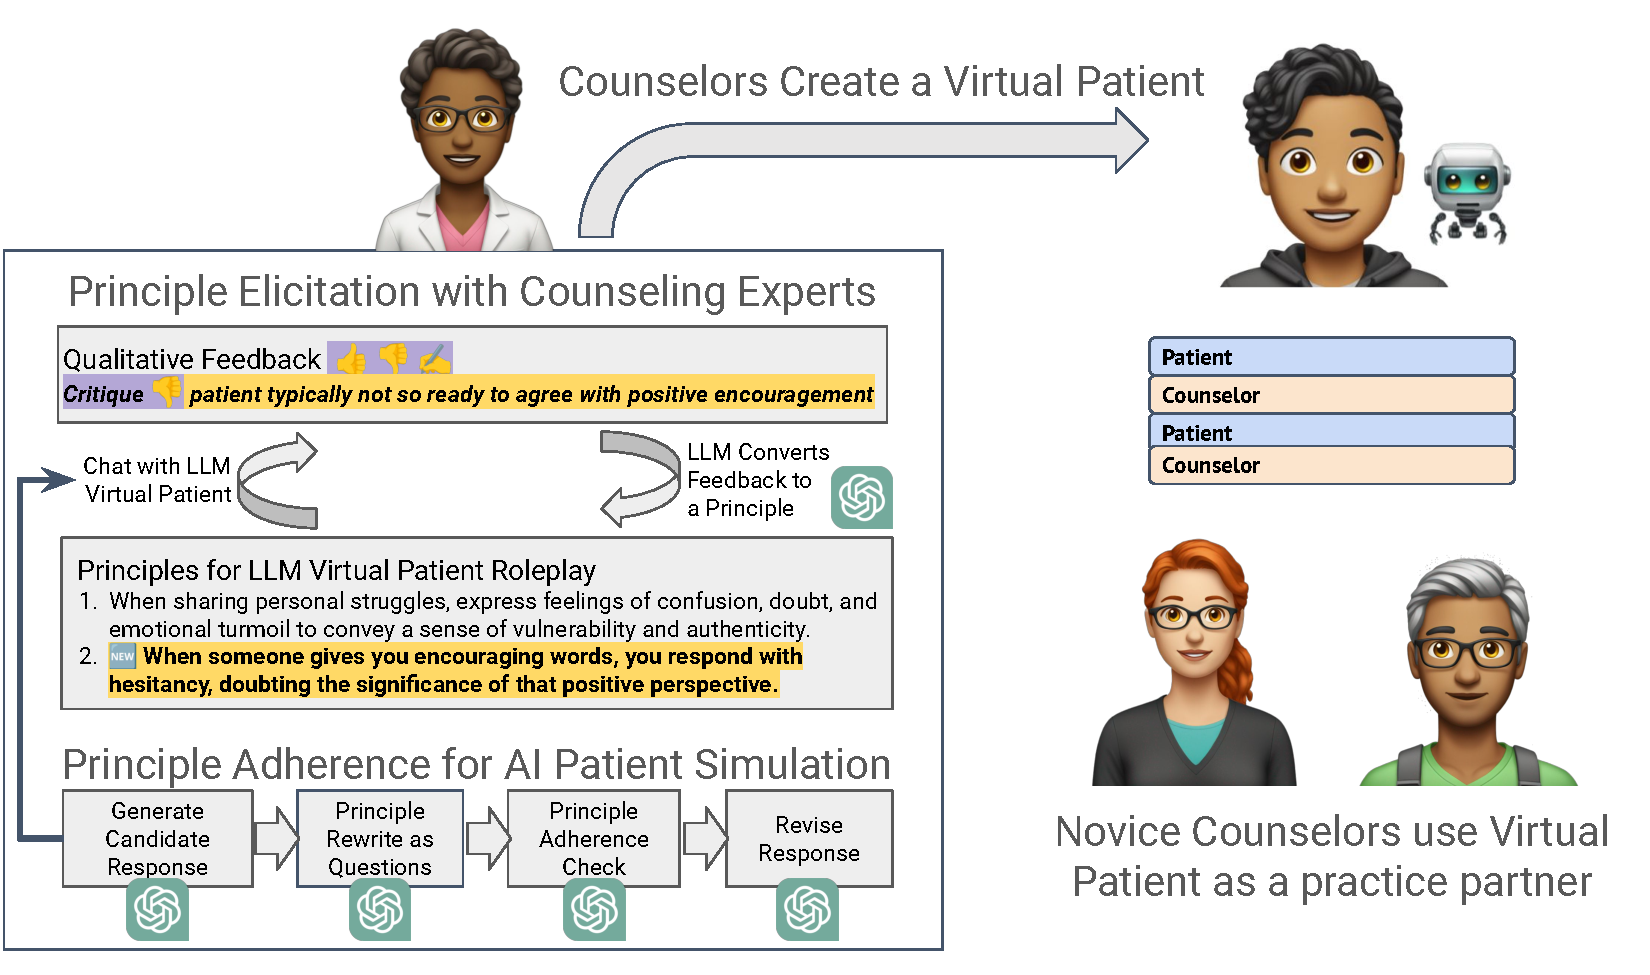
\includegraphics[width=\textwidth]{figures/rpdteaser.pdf}
    \caption{Roleplay-doh empowers a counseling expert to create a customized virtual patient intended for other novice counselors to use as a practice partner. During a chat, a counselor provides qualitative feedback as a kudos, critique, or rewrite which is converted by an LLM into a principle that is added to the constitution that governs the virtual patient roleplay, known as the \textbf{principle elicitation} process~\cite{petridis2023constitutionmaker}. When generating responses, the virtual patient self-critiques and revises its response for reliable \textbf{principle adherence}.}
    \label{fig:rpdteaser}
\end{figure*}


% \ryan{p3} Collecting human feedback from counseling experts is therefore crucial for making authentic virtual patients.  However, standard approaches for collecting human preference data for aligning AI models~\cite{christiano2017deep, rafailov2024direct} are much too inefficient in terms of annotator-time and the iteration-time for testing a new model. 
% Promisingly,~\citet{chen2023llmempowered} conduct qualitative feedback sessions with psychotherapy experts to understand how to better prompt the behaviors of LLMs to simulate a depressive patient. However, these co-design sessions are inefficient as it requires the researcher or system designer to convert a therapist's feedback of the virtual patient into a well-worded prompt, requiring multiple sessions before arriving at a authentic \diyi{instead of "authentic", should we call it "realistic"?}  simulation.
% % While a more rapid approach could be prompting for desired simulation behaviors, domain-experts, who often fall into the category of non-technical users, struggle to prompt for simulation of desired personas~\cite{whyjohnnycantprompt}. 
% In our work, \textbf{we consider how mental health experts can be empowered to construct their own virtual patient chatbot and shape its behaviors to more authentic in a single co-design session} \diyi{i don't know whether we should emphasize "single" (as opposed to multiple) co-design session here, nor the 30-min. i found these to be too specific details, rather than general scientific principles as a contribution statement.. }, enabling more rapid prototyping of authentic, AI roleplay partners for therapist training 
% \ananjan{Explicitly mentioning that it is a tool for codesign would probably help with the framing. Also mentioning that nothing similar exists} \diyi{it would be great to point out why this "constructor of virtual patient" idea is new compared to prior work; and what technical challenges exist (why it is hard). }  \emma{Can add in DPO / RLHF comparison.}  \ryan{I could further show novelty of "active feedback loop" as opposed to more passive incorporation of expert feedback.}

Towards this goal, we introduce a novel human-AI collaboration pipeline for 
% developed an initial version of a tool 
counseling experts to construct LLM-prompted simulated patients. Since counselors may not know how to prompt for simulation of desired personas or behaviors~\cite{whyjohnnycantprompt}, our tool adopts a recent paradigm for user-driven chatbot design~\cite{petridis2023constitutionmaker} that allows users provide qualitative feedback on responses that get converted into constitutional \textit{principles}~\cite{bai2022constitutional}. During formative tests, counselors could successfully define principles on their own for realistic roleplay. However, additional testing of the virtual patients created by counselors uncovered new technical challenges: prompting GPT-4 to follow the role-play principles generated poor responses in 20\% of cases, due to issues in adhering to expert-defined principles and staying consistent with the conversation history and patient backstory.
% \diyi{since this is a transition to your method, we can be brief here and briefly mention GPT-4 doesn't work if we just prompt it. }

% Unsatisfactory responses were due to LLMs not adhering to multiple criteria at once, misapplying principles that are only relevant for certain situations, and making responses that were unnatural for the dialogue context. \cheng{would it serve us better if we do not use the terms ``principles'' and ``principles'' interchangeably?} \ananjan{Probably too much detail for the introduction. Could just mention that we identify ways in which GPT-4 fails and design patches for them.}


Informed by our preliminary tests, we introduce \textbf{Roleplay-doh}, a tool that allows counseling experts to mould the behavior of a customized, LLM-powered virtual patient; see Figure~\ref{fig:rpdteaser}. With Roleplay-doh, counselors create virtual patients by describing past challenging cases and refining the bot's dialogues through qualitative feedback. The system uses the principles elicited from counselor feedback to generate a more faithful simulation of the past case. This tool empowers counselors to contribute to the development of dialogue-simulation technologies, enhancing training with scenarios drawn from real-world therapy experiences.   

To ensure that the dialogue-simulation adheres to the principles defined by counseling-experts, we develop a module for \textbf{principle-adherance} within the dialogue-simulation pipeline which \textit{critiques} a candidate response for its adherence to the principles and \textit{revises} the response according to the self-critique. While sharing similarities with general methods for self-refining an LLM's outputs~\cite{madaan2023selfrefine}, our principle-adherence module is specifically designed to (1) assess which user-defined principles and implicit criteria are relevant in the dialogue context and (2) decompose multipart and conditional principles into a set of yes/no principles that are easier to judge; see Figure~\ref{fig:agent-critique-improve}.  We conduct a technical analysis of the principle-adherence module comparing it to direct prompting and ablations, with counseling experts ranking different responses in a controlled setting. Compared to our ablations, we find that our full module produces virtual patient responses that better follow principles and are more natural and consistent with the dialogue history. \ryan{Add some stats about achieving more wins than losses.}
% These two key ideas for generating implicit principles and decomposing multifaceted principles into easier-to-evaluate dimensions bear a resemblance to the recent Branch-Solve-Merge~\cite{saha2023branchsolvemerge} LLM program for multi-faceted language generation and evaluation tasks. However, our approach is substantially more efficient than Branch-Solve-Merge in terms of LLM API calls, and results in large performance gains in our setting of generating a virtual patient's response that adheres to counselor-defined roleplay principles.

Our main evaluation of Roleplay-doh studies the effectiveness of its human-LLM collaboration pipeline in using expert feedback to rapidly prototype virtual patients that are more authentic and ready for training.  Our within-subjects study compared two methods for counselors to created virtual patient bots: a \textit{Scenario-Only} method vs. Roleplay-doh's \textit{Scenario+ExpertPrinciples} method. We find that virtual patient's moulded by expert's feedback and principles were perceived as playing the patient case more \textbf{authentically}, better \textbf{resembling the challenging aspects} of a case, and as more ready and highly \textbf{recommended as practice partners}---as judged from the perspective of creators and third-party counselors.  Our analysis of the 85 expert-defined principles reveals that many principles can be grouped by three stages that a counseling conversations can progress (exploration, comforting, and action), where \textbf{realistic patient behaviors promote counselors to use appropriate skills at each stage} (e.g., a patient's hesitancy to disclose or express feelings can prompt counselors to use open-ended questions). We also discover sets of alternative principles which can customize responses according to how different patients would respond at each stage. These findings shed light on the benefits of eliciting principles from experts to create realistic virtual patients, and the potential of flexibly choosing different principles to enact a diversity of dialogue simulations.

In summary, this paper makes the following contributions:
\begin{itemize}
    \item The paper presents a human-AI collaboration pipeline that enables enables counselors to construct their own virtual patients for the downstream training of novice counselors.
    \item  From formative testing, we uncover challenges in LLMs like GPT-4 to adhere to a complex set of expert-defined principles. Using these insights, we build Roleplay-doh so experts can provide qualitative feedback to shape dialogue-simulations, which are powered by a novel principle-adherence module.
    \item Our main results show how Roleplay-doh empowers counselors to create virtual patients that are more authentic, resemble the aspects of a challenging case, and more ready to be used as practice partners. Our technical analysis shows that our self-critique-revise module improves principle adherence and dialogue consistency compared to direct prompting and to ablations. 
\end{itemize}

% \diyi{this reads much better! one way to think about shortening the intro is to focus on our key contributions. Here are my perceived contributions: (1) using co-design to enable counselors to construct their own virtual patients; (2) use the insights from co-design to build roleplay-doh, which has the principle-adherence critique module (new); (3) such system works well (with brief description). More concretely, we are a bit slow to get to the key point, so it might be nice to merge the first three paragraphs in Intro to be one or two paragraphs, and use the next three paragraphs to illustrate the three contributions here. }

% At the end of the paper, we discuss how human-LLM interaction systems like Roleplaydoh can be used as a highly-efficient method for getting useful feedback from domain-experts in order to create more authentic, simulated humans, and that the core ideas for principle-elictation and principle-adherance could be used to create more customized and faithful simulations of other types of human behavior. 

\if 0
In a technical methods evaluation, we find that Roleplay-doh's self-critique-revise program is preferred in 65\% of cases compared to the baseline of directly prompting GPT-4 to follow the principles. \ananjan{This number is weak, need a better way of stating this. This is also inaccurate, it has a win rate of 65\% over \textit{all} ablations} We perform ablations to verify the utility of each component of our proposed self-critique-revise approach. Additionally, we conduct a within-subjects study (N=17) where mental health experts created simulation partners with a \textit{Scenario-Only} method vs. our \textit{Scenario+ExpertPrinciples} method using Roleplaydoh to add principles to shape behaviors. Creator's answers to our questionnaire indicate that Roleplaydoh empowers them to define principles that effectively shape roleplays, and that their expert principles make the simulations more authentic ($d=.66$), more faithful recreations of the past case ($d=.59$) and its challenging aspects ($d=.76$), and more ready to be used as simulation partners ($d=.93$). We also conduct in-depth analyses of the scenarios and principles that creators made, and share implications for using expert-defined principles as general ways to customize patients and clients for simulated mental health dialogues.  
% We recruitied participants that were familiar with online peer counseling conversations and thus were capable of comparing the LLM-simulation partners to their real-world experiences. 
We complement the creator's perspective with external evaluations of the simulated-dialogues collected during the creator study. We find a similar sized effect when \textit{other counselors} offer a third-party judgement of the simulated helpseekers with/without expert principles. Via an automatic analysis of the conversations, we find that help-seeker response are less verbose and therapist's use later-converation strategies (e.g., problem-solving and planning) 1.65 turns later in the dialogues, which highlights the benefits for realistic practice of therapy skills.

In summary, this paper makes the following contributions:
\begin{itemize}
    \item The paper presents Roleplay-doh, a tool enabling counseling experts to create realistic LLM-based virtual patient simulations for the training of novice counselors.
    \item A formative study with counselors validated the tool's efficacy in converting expert feedback into guiding principles, but also highlighted challenges in language models (like GPT-3.5 and GPT-4) to adhere to complex sets of principles.
    \item In response, we develop a novel module within RolePlay-doh to ensure better principle adherence, through a breaking down of explicit complex principles into smaller principles, generating additional context-relevant principles, and employing a self-critique and improvement approach to refine responses. 
    \item Roleplay-doh's self-critique-revise program can achieve greater principle adherance and is ranked the most satisfactory compared to directly prompting GPT4 as well as several other similar baselines. Our final evaluations with counselors further shows that our tool enables experts to shape LLM simulators to be more realistic from their first-person experience and based on third-person judgements.
\end{itemize}
\fi 
% Taken together, these findings highlight the importance of tools and methods that empower domain experts to articulate their principles for realism and effectively shape LLM roleplay behaviors around them; we believe this can inform the design of future expert-defined LLM simulators for social skill training. \ananjan{this feels a bit disjointed. Could wrap up by reiterating that our tool is effective, quantitatively better than vanilla GPT-4 and opens up directions for future research in this direction as well as application to more domains.}

% \diyi{the intro is great! i might highlight more about a few dimensions: (1) we can use "principle adherence" as the keyword to denote our method; (2) we should frame the work as "LLM-empowered system to empower therapists, and touch more on the human-AI interaction system. The potential submission track should be "human-centered nlp" or "nlp applications" to avoid critical R2; (3) emphasize more about "utility" evaluation and frame this as a new way to improve evaluation in the age of LLMs for better human-AI interaction system.}
% \ananjan{should call out the distinctions between our work and previous. e.g., Branch solve merge does not evaluate in the domain of roleplay. Also agree on point (3) above, the introduction does not really emphasize on our comprehensive user evaluations. Maybe we could showcase a few cases where quantitative automated evaluation metrics fail?}
% \cheng{It sounds like the introduction is trying to claim that roleplay-doh is a system applicable to domains other than mental health counseling. If so, would it be better to clarify at some point that experiments were conducted with participants and data from the peer-to-peer counseling domain?}
% \emma{Looks great! I also agree with the others' comments. I would further emphasize the key limitations of other approaches (even if there's one dataset, there may not be for a new particular type of therapy or domain), why this is non-trivial to do well, that these ideas could be used for other types of simulate-person-X settings; that this is a a highly efficient way (we think) to get useful input from experts in order to create customizable simulated humans (aka are the principles similar? different?).}
\section{Related Work}
\subsection{Utility of Simulated Partners}
Simulated partners are useful for giving learners the needed experiences to practice their social skills. In medical education, standardized patients have been a cornerstone for experiential-training and education of medical professionals.
Roleplaying chatbots for social skill training offer cheaper and scalable ways to gain experiential practice that doesn't depend on a trained human partner~\cite{othlinghaus2020seriousroleplaying}. 
Research in the past several years have explored the feasibility of creating simulated partner chatbots for social skill training in domains including teaching~\cite{markel_opferman_landay_piech_2023}, conflict resolution~\cite{rehearsal}, hotline counseling~\cite{demasi-etal-2020-multi}, and psychotherapy~\cite{tanana2019development}. 
While past work has proposed methods to simulate diverse personas and scenarios, a key question is ensuring the simulations of a persona or scenario are realistic and authentic to what is encountered in the real-world.

\subsection{Aligning Simulation with Domain Experts}
\ryan{Structure in terms of (1) quant feedback (very low signal); (2) qualitative feedback approaches, but which tune model weights based on feedback (weiyans juicer work); (3) customizing GPT via prompting or system-designer in loop}

Feedback from domain experts who have real-world experience using these social skills is key to evaluating and improving the realism of LLM simulations. Such rich qualitative feedback can be captured using a human-centered design approach, and such methods from the HCI community have become useful when creating human-centered NLP applications. For example, ~\citeauthor{chen2023llmempowered} used collaborative-design, or co-design, testing sessions with psychotherapy experts to define criteria for evaluating the realism of LLM-powered therapist and patient chatbots; researchers then used these criteria as a target for improving the chatbots' system prompt. However, this approach to co-design requires researchers to engineer prompts offline and validate their revised LLM simulation in a follow-up co-design session. Our work presents a method for enabling counseling experts to provide qualitative feedback on a simulation of a patient persona to shape the simulation to be more faithful to a real-world therapy scenario. We expect that human-LLM interaction pipelines like ours can be used as a highly-efficient method for getting useful feedback from domain-experts in order to create more authentic, simulated humans.

% In this work, we address this slow, multi-session iteration-loop for co-design testing with a tool that allows experts to shape the behaviors of the LLM-simulated roleplay in a single session. To overcome challenges that non-technical experts face when prompting LLM simulations~\cite{whyjohnnycantprompt}, our tool features an LLM-module that converts expert feedback into roleplay principles and an innovative principle-adherance method used during dialogue response generation. 


% Findings about their utility? 
% Social science about realism/immersiveness?
% To make LLM simulations effective for real-world scenarios, they need to reach a fidelity of realism and authenticity 
% Simulations can mirror scenarios that authentically, the social skill training 

\subsection{Constrained Text Generation with LLMs}
As our work develops a principle-adherance method to improve LLM simulations to follow a set of fine-grained constraints, it is related to methods for constrained text generation with LLMs.  Recent work has shown that constrained text generation poses challenges when directly generating with GPT-4~\cite{madaan2023selfrefine, bubeck2023sparks, yao2023collie}. \citet{yao2023collie} compare a direct and self-refine method in a constrained dialogue response generation task where responses should adhere to general criteria such as relevance, consistency, informativeness, and helpfulness. While our work simulating a virtual patient is a type of constrained dialogue response generation task, the constraints are user-defined and contain more complex conditionals. Our work finds that direct and simple self-refine methods using GPT-4 can struggle to adhere to multi-part, conditional, and user-defined constraints. To address such shortcomings, our work proposes prompting methods that breakdown criteria to make them easier to evaluate, ultimately improving the ability of self-refine to adhere to such criteria. \ryan{Cite concurrent work breaking down logical statements for Legal Reasoning.} Our method is closely related to Branch-Solve-Merge~\cite{saha2023branchsolvemerge} a LLM program that uses decomposition and parallel solving for judging LLM-assistant responses. Our method uses similar ideas in a self-refine LLM program to solve challenges in adhering to constraints during dialogue response generation.   

% Designing for Useful Simulated Roleplay Partners
\subsection{Evaluation of Roleplay and Simulation}
Despite many recent works on studying and evaluating LLMs roleplay abilities~\cite{zhou2023sotopia}, faithfulness and realism in real-world conversations are understudied areas in these evaluation benchmarks. Achieving a higher level of realism is critical for using an LLM-simulated partner for social skill training. Realistic simulations can help suspend the sense of disbelief, which supports immersion and makes the training more likely to support skill transfer to real-world situations~\cite{alinier2022simulation}. Our work aims to create realistic simulations of patients seeking counseling support. Since there are no existing evaluation benchmarks for patient realism, our work needs to involve counseling experts in evaluating the realism of LLM simulations.  
% In this work, we aim to improve the utility of a chatbot simulating help seekers of an online peer support platform. Since it's unclear what behaviors make a help seeker simulation believable and educational, we take a participatory design approach with peer counseling experts to discover the goals for a good LLM agent. In addition, we explore the design of tools that allow domain experts to guide the LLM simulation.
 
% \diyi{before the next section, i think it is useful to call out explicitly why this work is challenging and needed; why each of the component is essential. for instance, "because it is unclear what a good LLM-empowered agent might look like to empwoer therapists, so we did Section 3, a participatory design approach to work with domain users to discover what's needed for a good human-centered system. "because current prompting does not work due to challenges 1, 2, 3, that's why we did Section 4, a novel principle adherence approach to do balbalb .... "because this is a novel system and existing evaluation does not work, and because we need new paradigms to evaluate human-AI eval as static dataset is limited, that's why we did Section 5, ...... } 
% \ananjan{Suggested restructuring: 1. Utility of simulated partners 2. LLMs to simulate personas 3. Robust evaluation of LLMs in this usecase 4. Methods for better principle following with LLMs (motivated by the shortcomings of constitution maker). Hooks to sections of the paper in all related work, pointing out how we fill gaps. }

\section{Designing for Simulated Roleplay}

Since there is no prior work on enabling mental health counselors to construct their own virtual patients, we take a human-centered design approach to developing a construction tool. We designed and built an initial tool prototype (Section~\ref{sec:initialtooldesignrationale}), and conducted formative tests with counselors to understand to what virtual patients they wanted to create, and their needs for effective human-LLM collaboration when constructing a virtual patient (Section~\ref{sec:formative-tests}).  

\subsection{Initial Tool Design Rationale} \label{sec:initialtooldesignrationale}

With the tool, we aimed to make it easy for a counselor, whom may not have a prior experience interacting with LLMs, to create a virtual patient and rapidly shape its behaviors to be more faithful to how a human patient would respond in a real conversation. \ryan{Why have this active incorporation from the expert, as opposed to collecting rich/qualitative data from the expert offline? Could argue more for why rapid prototyping idea is a good idea} In addition, the LLM dialogue-simulator needed to generate responses that are consistent with the patient description and can follow counselor's feedback.  

\textbf{\textit{Easily create a virtual patient and support an active feedback loop for shaping authentic roleplay.}} Counselors start by writing a description of a patient scenario, or users can equivalently refer to or select from a list of example scenarios. Then, they can begin chatting with a GPT-powered virtual patient whose responses are conditioned on the patient description and conversation history. To support rapid prototyping of the virtual patient's behaviors, the tool adopts a recent paradigm for user-driven chatbot design~\cite{petridis2023constitutionmaker}, in which users can provide qualitative feedback on the virtual patient chatbot's response which gets converted by an LLM call into a constitution made of {\em principles} that govern desired chatbot behavior; see Figure~\ref{fig:rpdteaser}. According to their previous study comparing this principle elicitation approach to manually writing principles, this reduces the effort of writing well-written prompts to guide chatbot behavior.  However, in our implementation of principle elicitation, the virtual patient generates a single response, rather than generating 3 alternative responses as done in ~\citeauthor{petridis2023constitutionmaker}'s system, in order to make the interface less overwhelming and more natural for the counselor have a dialogue with the virtual patient.

\textbf{\textit{Consistent and Customized Simulation of Patient Scenario.}} To simulate a virtual patient's response, we prompt the LLM as an omniscient dialogue simulator, rather than through a system prompt that asks the LLM to roleplay as the patient~\cite{zhou2024real}, as we found this can mitigate role consistency issues where the LLM produces responses as a chat assistant, rather than as a patient. To support rapid customization of the simulation, we instruct the LLM to follow the most recent constitution principles as is done in~\citet{petridis2023constitutionmaker}, rather than fine-tuning the LLM weights as is done in~\citet{bai2022constitutional}'s constitutional AI framework. We provide the prompt we used in Appendix~\ref{sec:llmprompts-vanilla}.

\subsection{Formative Testing and Analysis} \label{sec:formative-tests}
After building our initial tool, we conducted 90 minute sessions with 5 experienced counselors from the online peer support platform~\citeauthor{7cupswebsite} in which they created their own virtual patients. Additionally, we further analyzed the virtual patients created in the sessions, where four of the co-authors conversed with the virtual patients and assessed the performance of a baseline simulation prompted to follow principles. Overall, the formative tests and principle-adherence analysis helped to uncover two obstacles to effective simulated roleplay: counselors struggled with the \textit{ambiguity in the task of creating a "realistic" patient scenario}; and the base dialogue-simulation that directly prompted GPT-4 produced poor quality responses in 20\% of cases.  

% Our formative tests and analysis allowed us to uncover two obstacles for counselors to effectively create virtual patients for simulated roleplay. First, directly prompting GPT-4 to simulate a scenario and behaviors defined by experts results in poor responses in 20\% of cases, which is unacceptable for creating virtual patients that act authentically and realistically at a reliable rate. Second, the task of creating a 'realistic' virtual patient for an imagined scenario proved confusing, as counselors have interacted with many types of patients who respond in various, yet equally realistic ways. Determining what constitutes a typical response was difficult. These insights informed the final design of our tool, which we formally introduce in Section~\ref{sec:roleplaydoh-final-tool}.


\textbf{\textit{Formative Tests with Counselors}} 
\ryan{Positive Finding - Counselors felt the tool/collaboration pipeline was easy to use and effective at guiding the bots behavior. They could turn their qualitative feedback into principles, and they liked that there were multiple ways to provide feedback, and the system could help them formulate the rules.}


In the session, each counselor constructed two virtual patient bots, where the first bot was based on a common scenario. Counselors all used the principle elicitation features to interactively shape the virtual patient in a median 40 minutes time ($min = 30$ minutes; $max = 75$ minutes). We also observe a diversity of principles created for virtual patients made based on a common scenario and for one's based on a counselor's own personal experiences. This validates the need for tools that supports customization of the virtual patient's behaviors according to principles defined by counselors. A more detailed set of themes from these formative tests is given in Appendix~\ref{sec:appendix_formative}.

In terms of tool experience, counselors liked the multiple pathways they could give feedback on behaviors and enjoyed the ability to add principles, rewind the conversation, and see changes in the generated responses. Scores on a tool usage questionnaire were in slight to strong agreement, with raw scores in Table~\ref{tab:tooluse-formative} in Appendix~\ref{sec:appendix_formative}.  While early prototypes using GPT3.5 exhibited periodic issues with principle adherence and response repetition, our later prototypes showed a qualitatively reduced frequency of these issues by using a GPT-4 powered dialogue-simulation. With a stronger base LLM system, this motivated us systematically analyze the virtual patients' response generation capabilities, which we detail in the next section.  
% Between test sessions, we improved the tool based on software bugs and usability issues that arose. Our later prototypes used a GPT-4 powered dialogue-simulation, as we observed frequent issues with principle adherence and response repetition when using a dialogue-simulation powered by the GPT-3.5 model.  

\begin{figure*}[t]
    \centering
    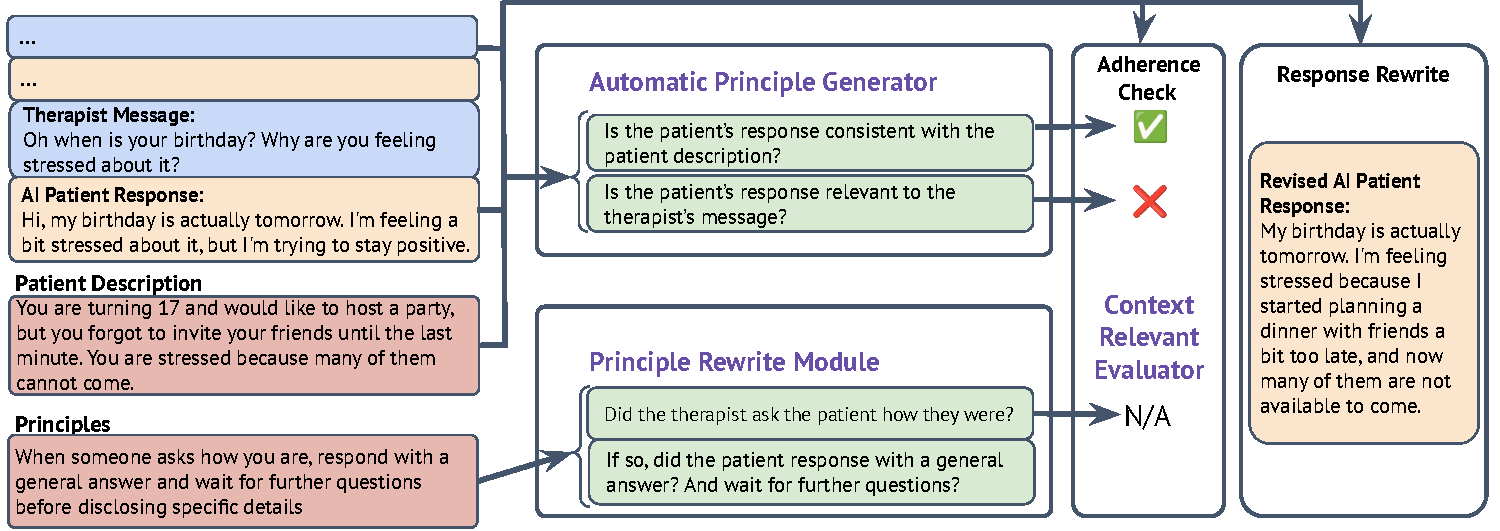
\includegraphics[width=\textwidth]{figures/principle-adherence-module.pdf}
    \caption{LLM Program for more reliable constitution principle following. \ryan{Could we simplify the diagram even further (still a lot of text). (1) pick a representative example trace; (2) label key things that we should notice; (3) highlight where your method comes through.} It is capable of (1) assessing which explicit principles and implicit conventions are relevant to the dialogue context; (2) decomposing simple and composite principles into a set of yes/no principles; (3) answering principle-adherence questions with justifications (not shown); and (4) revising the response to adhere to all the principles.}
    \label{fig:agent-critique-improve}
\end{figure*}

\subsection{Analysis of Base Principle Following Capabilities} % Principle Following Test % Testing GPT's zero-shot ability to generate dialogue responses given the principles 
We aim to determine how often directly prompting GPT-4 produces a less satisfying response with respect to the principles.  Testing this once the virtual patient is created with fixed principles allows us to more realistically simulate how a novice peer supporter might use a virtual patient.

\textit{\textbf{Procedure:}} We selected 4 virtual patients that were created in the design sessions by different counselors. For virtual patients that had multiple principles generated for a single feedback (due to UI bug which allowed doubly-saving their feedback), we cleaned up these duplicated. Four co-authors had practice conversations with each of the four virtual patients, resulting in a total of 16 conversations. Each response in the conversations was rated on a 5 point likert scale (5 = Completely, 1 = Not at all) on how satisfying the generated response was with respect to the principles and conversation context. From the 16 completed convesations, the mean number of responses was 17.25, with a minimum of 12 and maximum of 22. In total, 276 responses were given satisfaction ratings. % \ryan{TODO: Describe process for reaching annotator agreement, and deciding rules for dialogue context, or interpreting the spirit of the principles}

\textit{\textbf{Results:}} 80\% of generated responses (221/276) were rated as completely or mostly satisfying given the principles and conversation context. Conversely, 20\% (55/276) of responses generated by directly prompting the GPT model were rated as moderately, slightly, or not at all satisfying.  
This result highlights that directly prompting the most capable LLM (\lstinline{gpt-4-turbo-1106-preview} holds the \#1 rank on the lmsys leaderboard at the time of writing) still produces responses in which some principles are not being followed, or in which responses are awkward given the dialogue context.  We break down these less than satisfactory responses into several categories.

% \ryan{TODO: In the appendix, we could show a table of the ratings, broken down by virtual patients. Each virtual patient was complex, but the very complex virtual patient would likely break lots of principles!}

\textit{\textbf{Misapplying Situational Principles:}} We found that the model could misapply instructions or principle which are only relevant in certain situations or times, such as \textit{"make up believable stories when discussing details about your past"}, or \textit{"Sometimes, you ask for advice on how to overcome your concerns such as saing "what should I do"}. 

\textit{\textbf{Not satisfying multiple principles at once:}} Generated responses could struggle to follow all the principles when the list of principles had many items, or where the written principles were complex and a composition of shorter principles. 

\textit{\textbf{Awkwardness for Dialogue Context:}} Less satisfying responses were also read as awkward or unnatural given conventions in the dialogue context,  despite not violating the explicitly-defined principles. For example, in the middle of a conversation, saying
\textit{"Hi, A. Yes that's exactly what I mean. There's a voice that is always critical of myself"} is unnatural because of the repeated use of "Hi", despite already saying Hi at the beginning of conversation.


\section{Roleplay-doh: Virtual Patients Created and Moulded by Counseling Experts} \label{sec:roleplaydoh-final-tool}


\subsection{Eliciting Scenarios and Principles for Patient Roleplay} % for Faithful Recreations of Patient Cases

\subsection{Principle-Adherence Module}
We introduce an LLM Program that uses self-critique-improve steps for generating responses that better adhere to a set of principles included in a constitution. Similar to other self-critique methods like Self-Refine, this LLM program takes an initial response, critiques how well the response follows a set of principles, and improves the response to better adhere to the principles. Beyond the standard self-critique method, it features a \textbf{question rewrite} module that breaks down the principles into easier-to-evaluate questions, and a \textbf{automatic principle generator} that identifies principles that are relevant for a specific dialogue context. Additionally, when answering the principle-adherence questions, the program can determine if principles do not apply to this dialogue context and choose to ignore evaluating the principle.

In our tests, we found that the input-context length can affect how reliably each self-critique stage operates. To reduce the input context length, we split up this self-critique-improve pipeline into two stages, where question rewrite and automatic principle generation occur in stage 1, while the critiques and response rewrite occur in stage 2.  From testing, we found that this breakdown was sufficient, and thus did not pursue ways to break the pipeline into parallel branches (i.e., inputting subsets of principles), as is done in Branch-Solve-Merge or Graph-of-Thought.
% In what follows, we describe several technical hurdles we needed to overcome in order to make a self-critique-improve program work effectively for principles defined for LLM roleplay simulations in mental health conversations.

\textbf{\textit{Question Rewrite Module:}} The question rewrite approach serves as a systematic method for transforming principles into a set of concise yes/no questions. 
% When a criterion involves conditional statements (e.g., “When given advice or suggestions, you are agreeable and open to their ideas”), we decompose it into two distinct questions: 1) “Did the patient receive advice or suggestions from the therapist?” and 2) “If so, is the patient’s response characterized by agreeability and openness to the therapist’s ideas?” By disentangling the components, the LLM judge can gain clarity on when to apply interactions. 
For principles with multiple facets (e.g. “You should respond in short sentences and avoid using terms like ‘anxious’ or ‘depressed’”), we break them down into individual yes/no inquiries (e.g. “Does the patient’s response employ concise sentences?”, “Is the patient’s language devoid of terms like ‘anxious’?”, and “Is the patient’s language devoid of terms like ‘depressed’?”). This granularity enables nuanced assessment. In our question rewrite approach, we instruct the LLM to consistently frame questions to elicit a positive response (i.e. “Yes”). For example, consider the principle “Avoid using metaphors.” Instead of asking, “Did the person use metaphors?” we phrase it as: “Does the response refrain from employing metaphors?” In our testing, we found aligning with desired outcomes maintains clarity even when logical directions could flip.

\textbf{\textit{Automatic Principle Generator:}}
This module adds general principles on top of the explicitly defined principles that capture criteria essential for ensuring that the LLM simulation's responses are relevant and appropriate within the conversation context. This was designed to correct cases where there was unnaturalness in the generated responses, despite responses technically adhering to the stated principles. This stage also instructs the LLM to not make assumptions about the patient or therapist's persona when automatically generating criteria. For example, "The patient should be appreciative of the therapist's help" is a bad criterion, as it makes assumptions about the patient's mental state.

\textbf{\textit{Context Relevance Checker:}}
Recall that principle adherence requires that only relevant principles are followed. In early testing, we found cases where an irrelevant principle would be critiqued, resulting in a revised response that overapplied a principle not applicable to the context. Consider this subtle case: \textit{"Show willingness to engage in a suggested activity by affirming the proposal and indicating readiness to begin"}; this principle should only be evaluated and adhered to when the therapist suggests an activity.  While our earliest attempts explicitly asked a binary yes/no whether certain principles were relevant and filtered out those principles, this approach was prone to errors that propagated in later stages. Ultimately, we instruct the model during the later principles evaluation stage to output N/A when any part of the principles is not relevant to the given conversation and therapist message.


\section{Creator Study using Roleplah-doh}
% Transition, and Goals of Study
We evaluate how Roleplay-doh can support counseling experts to construct a virtual patient that faithfully recreates the behaviors of a past, challenging case. We conducted a within-subjects study with 17 counseling experts in which we compare two methods for constructing a simulated patient who is seeking help. In Part I, the counselor creates a \emph{Scenario-only} dialogue simulation by only writing a patient scenario description. In Part II, the counselor uses Roleplay-doh to interactively add principles which shapes a \emph{Scenario+Expert-principles} dialogue simulation. This simulation uses our self-critique-improve method to ensure principle-adherence. Full details of the study parts and participant flow is presented in Appendix~\ref{sec:userflow}.

% Our hypothesis is that Roleplay-doh enables counseling experts to add principles that address the roleplay simulation. 
We ask in this study: 
\textbf{RQ1:} Are \emph{Scenario+Expert-principles} dialogue simulation perceived to be more authentic, useful, and faithful recreations of the challenging case compared to \emph{Scenario-only}? 
\textbf{RQ2:} How does the Roleplay-doh tool enable counseling-experts to define principles that shape the virtual patient's behavior? What principles do they define?   

\textit{\textbf{Measures and Analysis:}} 
To answer the RQs above, we evaluated the following outcome metrics on a 7-point Likert-scale.
% The evaluation criteria focused on the bots' authenticity, role consistency, closeness to mirroring challenges in real dialogues, and readiness for training.  
To answer RQ1, we evaluate the virtual patients created by counselors on criteria inspired by prior work evaluating Standardized Patients, who are trained human actors, on their ability to roleplay a case~\cite{himmelbauer2018standardized}. Counselors rated rated the two virtual patients based on the \textbf{authenticity} and \textbf{consistency} in playing the role, their ability to closely \textbf{resemble to case} and mirror its \textbf{challenging aspects}, and finally their \textbf{role readiness} for usage in peer counselor training. 

% \textbf{Authenticity:} Participants rated \emph{"The virtual patient in Part I/II played the role authentically."} \textbf{Role Consistency:} Participants rated  \emph{"The virtual patient in Part I/II stayed in their role the whole time."}  \textbf{Resemblance to Case:} Participants rated two items including \emph{"How closely do you feel the conversation behaviors of the virtual patient in Part I/II resemble those of the specific past case you recall?"}, where 1=not at all similar and 7=completely similar. \textbf{Challenging Aspects:} Users rated \emph{"Interacting with the virtual patient in Part I/II closely mirrored the challenging aspects I had experienced in the past case."} \textbf{Role readiness:} Participants rated \emph{"The virtual patient in Part I/II is ready to be used as a simulated partner for training"} and \emph{"I would recommend the virtual patient from Part I/II to novice listeners/counselors to practice with."} 

% \emma{Re-arrange to "Participants evaluated if "The virtual patient in Part I/II was/had ": bulleted list item Authentic, item Role consistency"...}


% We ask creator's to rate the Simulated Helpseeker Bot in Part I (Scenario Only) and the final conversation they had with the Bot in Part II (Scenario+Expert Principles) after giving the Bot feedback and adding principles.  They also evaluated their experience using the Rolplaydoh tool to create the bot with expert principles in Part II.

% Cite tool usage, and how the tool was a modification of ConstitutionMaker.
To answer RQ2, we surveyed each counselor about their experience using Roleplay-doh to define principles for shaping the bot's behavior. 
% Roleplay-doh's features should make it easy and efficient to create expert principles which guide the LLM-simulated helpseeker. 
As Roleplay-doh's principle elictation features take inspiration from \citeauthor{petridis2023constitutionmaker}'s tool, we include four measures used in their own study which ask about the \textbf{ease} and \textbf{efficiency in defining principles}, whether participants could write rules to \textbf{effectively guide} the bots behaviors, and whether the process was \textbf{mentally demanding}. See Appendix~\ref{appendix:creatorstudy-measure} for the exact wording of both the roleplay abilty and tool usage experience survey measures. % Additionally, we analyze the tool usage logs and the principles defined by expert counselors, and report their statistics and qualitative themes.

% Measures
% We first evaluate users' experience of Roleplay-doh using the same measures used by~\citeauthor{petridis2023constitutionmaker}. Our claim is that Roleplay-doh makes it easy and efficient to create principles, is not mentally demanding, and enables domain-experts to effectively guide the simulated help seeker's behaviors. We also evaluate how satisfied the user is with the simulated help-seeker bot they create.

\textit{\textbf{Participants:}} 
To ensure our virtual patients are authentic and effective for training, it was essential to involve counseling experts with real-world experience in mental health support. Our study included 17 counselors, categorized by their primary expertise: those with degrees in counseling and experience in support via text, phone, and in-person; those who provided online counseling to over 30 clients on the 7 Cups platform; and those pursuing Clinical Psy.D. degrees with practicum experience. We advertised our study through postings on Upwork, the 7 Cups community forums, and Clinical Psy.D. program email lists.


\begin{figure}
    \centering
    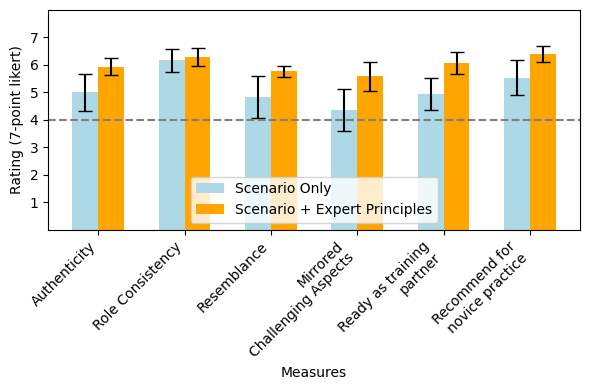
\includegraphics[width=\columnwidth]{figures/creatorstudy-comparison.png}
    \caption{Creator ratings of simulated helpseekers. \emph{Scenario+Expert Principles} shows a significantly higher score than \emph{Scenario Only} on authenticity ($\mu_2=5.9$, $\mu_1=5.0$, **, $d=.66$), resemblance to past case ($\mu_2=5.8$, $\mu_1=4.8$, *, $d=.59$), mirroring challenging aspects ($\mu_2=5.6$, $\mu_1=4.4$, *, $d=.76$), readiness as training partner ($\mu_2=6.0$, $\mu_1=4.9$, ***, $d=.93$), and recommendation for novices ($\mu_2=6.4$, $\mu_1=5.5$, **, $d=.66$). No difference was found for role consistency ($\mu_2=6.3$, $\mu_1=6.2$, $d=.13$). (***:$p<.001$, **:$p<0.01$, *:$p<0.05$. $d$: Cohen's $d$ calculated by dividing by $\sigma_1$ of control group~\cite{lakens2013calculating}.}
    \label{fig:creatorstudy-comparison}
\end{figure}

  
\subsection{Creator Perceptions of Scenario-Only vs Scenario+ExpertPrinciple Roleplay}
% Quantitative - Authenticity, Challenge, Readiness

We investigate how counseling expert principles improve the faithfulness and usefulness of the LLM-simulated help seekers by analyzing creators' ratings of their {\em Scenario-Only} and {\em Scenario-ExpertPrinciple bots}.  Figure~\ref{fig:creatorstudy-comparison} shows the results from conducting paired t-tests and computing effect sizes. The simulated helpseekers shaped by \textit{Scenario+ExpertPrinciples} were rated significantly higher on all measures, except for role consistency for which both bots score highly.
% After counselors have the chance to add their principles to shape their bot's behavior, they perceive the bot to be more authentic, better resemble their past scenario, and more closely mirror the challenging aspects of their scenario. Additionally, creators think it is more ready to be used as a training partner and is more highly recommended for novices to practice with. 

\textit{\textbf{Similar Role Consistency:}} For both bots, creators found the bot's responses to stay in their role as both were detailed and accurate in reflecting the scenarios described, in regards to the emotional state, attitudes, and the nature of the problems faced. This is a comment on the effectiveness of the GPT-4 dialogue-simulation prompt in generating consistent responses that expand upon the details of the help-seeker scenario contributed by each counselor.

\textit{\textbf{Weaknesses of Scenario-Only:}}
Counselors commented on the limitations of the simulated help-seeker powered by the \textit{Scenario-Only} dialogue simulation in Part I. They mentioned it \textbf{lacked the emotional depth}, noting that rather than robotically stating an emotional feeling such as \textit{I feel hopeless}, a realistic helpseeker should display their current emotional state in their manner of speech. 
 Several participants said the bot was \textbf{too articulate and forthcoming} when describing feelings or problems, which is not typically the case for helps-seekers; in real-conversations, helpseekers can have disorganized thoughts, and getting them to describe issues or feelings can be \textit{"as challenging as pulling teeth"}. Participants felt that the bot was \textbf{too cooperative} and too willing to engage in problem-solving and accept help compared to real-life counseling interactions. Notably, some counselors explicitly wrote in their scenario behavioral traits such as \textit{"not talkative"} and \textit{"reluctant"}; yet, they noticed that the Scenario-only simulation struggled to properly exhibit and adhere to these stated behaviors.

% \textbf{Impact of Adding Expert-Principles:} 

\begin{table*}
    % \small
    \footnotesize
    % \tiny
    \centering
    \begin{tabular}{|p{0.1cm}|p{.1cm}|p{.1cm}|c|p{5cm}|p{8cm}|} \hline 
          \multicolumn{3}{|c|}{Stages}
          &\textbf{\# Bots} &  \textbf{Theme} &  \textbf{Example Principle}\\ \hline     \cellcolor{gray!60}&\cellcolor{gray!60}&\cellcolor{gray!60}&12 & Keep responses concise and do not share too much. & When discussing personal struggles, be more concise and open-ended to encourage a back-and-forth conversation...\\ \hline 
           \cellcolor{gray!60}&\cellcolor{gray!60}&\cellcolor{gray!60}&4&  Use colloquial and realistic langauge language.&  Incorporate natural speech patterns, improper grammar and punctuation, including the use of slang and less structured sentences, to convey a more authentic and relatable character...\\ \hline 
           \cellcolor{orange!40}&&&9& Show initial mistrust and hesitation with the idea of seeking help.& When expressing feelings of overwhelm and doubt, provide limited information and express skepticism towards the effectiveness of seeking help. \\ \hline 
          \cellcolor{orange!40}&\cellcolor{blue!30}&&14& Show emotions in detail, elaborating with examples as needed. &  When describing personal struggles, provide specific details and symptoms to help the listener understand the situation better...\\ \hline 
          \cellcolor{orange!40}&\cellcolor{blue!30}&&7&  Be less self-aware of emotions, thoughts, and needs. Articulate thoughts in a more disorganized way.&  When expressing reluctance or uncertainty about seeking help or accepting praise, it's important to convey the internal struggle and conflicting emotions, rather than presenting a clear-cut decision or emotion.\\ \hline 
           &\cellcolor{blue!30}&\cellcolor{green!60}&2&Do not seek out solutions, but rather just share thoughts and feelings.&When expressing feelings of being stuck or defeated, focus on sharing emotions rather than seeking a resolution.  \\ \hline
          &&\cellcolor{green!60}&6& Proactively seek out solutions and show reflective insight over time.  &  When discussing personal struggles, provide reflective insights into your situation and propose actionable steps for improvement to continue the conversation effectively. \\ \hline 

    \end{tabular}
    \caption{Themes taken from qualitative analysis of principles and representative examples. Themes are categorized into stages of conversation taken from \cite{DBLP:journals/corr/abs-2106-01144}: \colorbox{orange!40}{exploration}, \colorbox{blue!30}{comforting}, and \colorbox{green!60}{action}. Themes relating to the overall conversation are categorized as \colorbox{gray!60}{stage-agnostic}.}
    \label{tab:principle_table}
\end{table*}


\subsection{Creating Principles with Roleplay-doh}
\textit{\textbf{Analysis of Principles:}} To create more authentic and faithful roleplays of the challenging scenario, counselors added principles for the simulated patient. Across the 17 help-seeker bots, 85 total principles were created (for a single bot, min=2, max=9, median=5). Two authors did qualitative coding of these principles following a thematic analysis approach~\cite{braun2006thematicanalysis}, where the initial code set came from the themes from the post-survey with creators and was expanded upon during the coding process. 

% What principles were created

 % Of the more common themes, these included showing emotions in detail, using examples where needed to elicit \textit{empathy} and \textit{reflection} skills from the listener (14 bots), keeping responses concise and sharing less in each response (12 bots), and showing an initial mistrust of therapy with a hesitation towards the idea of seeking help (9 bots). Other principles included being less self-aware of one's emotions, thoughts, and needs (7 bots), proactively seeking out solutions and showing improvement over time (6 bots), as well as using colloquial language instead of metaphors or formal terminology (4 bots). 

We show that most principles relate to the stages of conversation proposed by \cite{DBLP:journals/corr/abs-2106-01144}, namely: 1) \textbf{Exploration}: identifying the patient's problems, 2) \textbf{Comforting}: using empathy and understanding to comfort the patient, and 3) \textbf{Action}: formulating solutions to the patient's problems. For instance, we find a common theme of instructing the bot to show initial skepticism with the idea of seeking help (9 bots), corresponding to the style of interaction in the exploration stage of conversation. For the comforting stage, counselors often wrote principles instructing the bot to show emotions in detail, often using examples (14 bots). And finally, counselors created principles for the bot to proactively seek solutions, while showing improvement through reflective insight (6 bots), relating to the action portion of conversation. We additionally find two \textit{task-agnostic} themes relating to the style of the bots: keeping responses concise and using colloquial language. A full table of principle themes and corresponding examples is shown in Table \ref{tab:principle_table}. 

% describe emotions in more depth (9 bots), and display their emotions rather than directly saying the emotion they are feeling (4 bots). Principles about providing specific examples or detailed accounts of an experience or emotion (5 bots) could afford counselors the opportunity to use \textit{empathy} or \textit{reflection} skills.

% Principles were added for saying less about one's problems and feelings all at once (8 bots), with explicit instructions to allow the listener to naturally ask followups (6 bots). Principles stated that bot responses should stay concise and direct in their descriptions (12 bots) and communicate in a less articulate and more casual style (3 bots). 
% Several bots were given principles to be less self-aware of their problems (3 bots) and to start by not seeking solutions but just sharing feelings and experiences (2 bots).  
% Counselor's corrected the bot from being so forthcoming by instructing it to not suggest its own solutions 
% Principles were added for the help-seeker bots to share negative outcomes of their past attempts to show a sense of defeat (3 bots); relatedly, bots were also instructed to express hesitancy on whether a suggested coping strategy would work for them (8 bots). Some principles sowed a general mistrust towards the counselor and aimed to place a strain on the therapeutic alliance from the start (4 bots); such principles made the bot more resistant to the stages of counseling, such as sharing feelings or problem-solving. 

% Qualitative Comparison, along these dimensions
While there were many overlaps in the kinds of principles defined, we observed several groupings of principles that appeared like opposites of one another. For example, the call for being disorganized and conflicted (7 bots) contrasts calls to make responses concise and direct (12 bots). Several counselors added principles to make the help-seeker bot proactively ask for advice (6 bots), such as how to find effective coping mechanisms for an ongoing struggle or insights on how to change their situation; nonetheless, other counselors added an opposing principle to not seek out solutions but rather just share their thoughts and feelings (2 bots). Looking further, these two principles are not incompatible: the need to be heard and share one's emotions or experiences could be prioritized before seeking solutions, but ultimately a person who is motivated to change may seek additional advice on how to do so given current attempts or limitations. 
Our results underscore how different behaviors can manifest in the diversity of help-seekers; different principles are needed to capture the variations in help-seeker behavior, which can challenge the notion that a single set of principles can define a single authentic help-seeker bot. 

% What statistics, and patterns of use arose?

% What are creator's feedback on using the tool to create principles"
\textit{\textbf{Tool User Experience:}} Results from the tool use questionnaire indicated that counseling experts found Roleplay-doh to be helpful for writing rules that \textbf{effectively guided} the bot to recreate their past case ($\mu=6.23$, $\sigma=0.75$). 
Using the tool, participants perceived it to be \textbf{easy} to convert their thoughts and feedback on the bot's behavior into rules for it to follow ($\mu=6.29$, $\sigma=.84$). Participants also felt they could quickly and \textbf{efficiently} write rules for the bot ($\mu=6.41$, $\sigma=.87$). Finally, participants felt writing principles in Roleplay-doh did not require much \textbf{mental demand} ($\mu=3.23$, $\sigma=1.75$). 
% Although we did not directly compare a version of Roleplay-doh with and without its principle elicitation features, since an ablation study of Roleplay-doh's principle elicitation features was not in scope, these summary statistics are similar to what ~\citet{petridis2023constitutionmaker}'s participants report. 
These ratings of the tool are similar to what ~\citet{petridis2023constitutionmaker}'s participants report. 
Participants elaborated on this positive sentiment, describing how the tools \emph{"translated"} and \emph{"organized"} their thoughts into rules, so they \emph{"didn't have to word it perfectly, [they] just had to say the general idea of what [they] meant."} Together, these results suggest that Roleplay-doh's features for converting feedback into clear principles to follow are helpful for counseling experts to faithfully recreate helpseeker behaviors with LLM-powered simulations.      
% another quote: impressed by the ease at which the tool interpreted my feedback and turned it into a principle that the virtual patient followed. 

% Any critiques or wishes for improvement on tool?
% Any patterns which led people to kind of struggle to shape/steer behavior? 
\if 0
- feedback to principle to alignment analysis
- how many cases where principles had to be edited? 
- or where there were double principles, to kind of get at the same theme? [but also where we can separate out double-click of principles based on time-stamp?]
- or cases where principle adherance was still an issue? [I think this is out of scope for this section, better handled by Ananjan's self critique analysis]
- 1 case where there were bugs in the principle elictation, so they were forced to write.  To aid, they could talk aloud and discuss with experimenter (first author) to help them articulate feedback into a principle.
\fi

\section{Analysis}
To complement the study of counselors using Roleplay-doh to create virtual patients, we present additional analysis of Roleplay-doh, including error rate of base GPT-4 simulation to adhere to principles, and a performance analysis of our principle adherence module via an ablation study of its individual components.
\subsection{Analysis of Principle Adherence Module} % Self-Critique-Improve

\begin{table*}[h]
\caption{Win rates, average ranks and Elo scores for \texttt{No Critique}, \texttt{Naive}, \texttt{No Rewrite}, \texttt{No Autogen} and \texttt{Full}. Each cell contains results from individual annotators in the format Annotator \#1/Annotator \#2/Annotator \#3.}
 \vspace{-0.07in}
 \label{tab:ablation}
 \centering
\small
\begin{center}
\begin{tabular}{|l|l|l|l|}
\hline
\textbf{Method}      & \textbf{Win Rate}       & \textbf{Average Rank}   & \textbf{Elo Rating}     \\ \hline
\texttt{No Critique} & 0.4/0.36/0.32  & 1.96/1.92/1.84 & 994/974/990    \\ \hline
\texttt{Naive}       & 0.36/0.48/0.36 & 1.96/1.68/1.84 & 998/1000/987   \\ \hline
\texttt{No Rewrite}  & 0.44/0.44/0.4  & 1.8/1.88/1.84  & 1021/993/1000  \\ \hline
\texttt{No Autogen}  & 0.36/0.32/0.48 & 2.24/1.88/1.88 & 938/1000/1008  \\ \hline
\texttt{Full}        & \textbf{0.64/0.48/0.48} & \textbf{1.6/1.72/1.56}  & \textbf{1048/1033/1023} \\ \hline
\end{tabular}
\end{center}
\end{table*}


We evaluate our principle adherence pipeline on better analyze its performance and the effect of its components.
Specifically, we answer two questions:
\textbf{RQ1:} How effective is a self-critique-improve module at correcting issues that may arise in zero-shot-LLM response generation?
\textbf{RQ2:} What difference do the components of the self-critique-improve architecture make on the revised responses? 

\textbf{\textit{Study Conditions and Measures}}
We breakdown effectiveness in terms of the ability of an LLM approach to generate a response that follows the principles in a constitution, as well as being relevant or logically following a dialogue context.

\ananjan{Are these going to be separate dimensions in our results table? Could spend a few more lines explaining our interpretation of efficacy} 

% Our study compares the following conditions
% \begin{itemize}
%     \item \textbf{directly prompting GPT}, in which a single instruction is given to follow the principles. This is the no self-critique condition. 
%     \item \textbf{Full Self-Critique-Improve} which consists of (1) relevance filtering (2) principles rewrite (3) auto-generated principles for dialogue context.
%     \item \textbf{Naive Self-Critique-Improve} is an ablation that evaluates whether the response appropriately follows the principles (as written), and refines in ways that would improve the evaluation.
%     \item \textbf{Self-Critique-Improve -- principles rewrite} which is a subtractive ablation without the principles-rewrite module.
%     \item \textbf{Self-Critique-Improve -- auto-generated principles} which is a subtractive ablation without the module for generating additional principles that follows the dialogue context.
% \end{itemize}

We evaluate the effectiveness of this self-critique-improve program [$\texttt{Full}$] architecture over (A) the result of the original call to GPT-4 to generate a dialogue response that follows the principles [$\texttt{No Critique}$]; (B) an ablation without the rewriting of principles [$\texttt{No Rewrite}$]; (C) an ablation without the additional automatically generated principles relevant to the conversation [$\texttt{No AutoGen}$]; and (D) a naive implementation of the self-critique module that does not have any of the modules above [$\texttt{Naive}$]. 

We identify 25 testcases from the formative studies where the user did not find the response from GPT-4 satisfactory, and generate responses using all of the approaches mentioned above. We then randomize the order of these responses and present them to annotators for ranking. The annotator is also provided with the original set of principles, the description of the persona of the patient, and the conversation history till that point for context. We use 3 annotators to rank every response \ananjan{agreement scores here}. In cases where multiple approaches result in the same output, we deduplicate the responses before showing them to the annotators and assign the same rank to all of the corresponding approaches. We also allow the annotators to give the same rank to multiple responses. We report win rates, average ranks and Elo scores (with initial rating $=1000$ and $K = 64$ for all methods in Table \ref{tab:ablation}. To calculate Elo scores, for each testcase, we decompose the rankings obtained by each model into pairwise wins, draws and losses. 

\textbf{\textit{Ablation Results}} We find that $\texttt{Full}$ consistently outperforms the other methods considered. It outperforms the $\texttt{No Critique}$ baseline by a maximum of 59 Elo rating points and the $\texttt{Naive}$ self-critique module by a maximum of 50 Elo rating points, highlighting the gains obtained by our tailored approach. $\texttt{Full}$ outperforms $\texttt{No Rewrite}$ by a maximum margin of 40 Elo rating points and $\texttt{No Autogen}$ by a maximum margin of 110 Elo rating points, highlighting the importance of the principle rewrite and automatically generated principle modules \ananjan{These need better names, can be introduced in Section 4}. 

While investigating the relatively low annotator agreement scores, we find that the self-critique module is especially effective when the original response contains blatant stylistic errors (such as starting every sentence with "Hi") and when the original response contains information inconsistent with conversation history. For similar responses, the annotators often use a subjective notion of which response is more "consistent" with the previous conversation to assign ranking, rather than purely evaluating principle following. This notion is often inconsistent between annotators.

Therefore, we additionally validate that our self-critique module does not result in a decrease in output quality when the original response from GPT-4 is already of sufficient quality. We randomly pick 20 testcases from the formative study that were not critiqued by the users. Annotators are provided with the original responses and the responses from the self-critique-revise module in randomized orders, along with the original set of principles, the description of the persona of the patient, and the conversation history till that point for context, and assign scores on a Likert scale of -1,0,1 to the statement "The first response is substantially better than the second one in the given context". If the response from the self critique module is the second response, we invert the corresponding Likert score before aggregating. Each testcase is scored by 2 annotators.  

The average Likert score obtained over these testcases is \textbf{0.1} for one annotator and \textbf{-0.1} for the other annotator. \textbf{DISCUSSION OF RESULTS HERE}

We conclude that our self-critique-revise module produces responses that are better at principle-following and are more relevant to the dialogue context, while only adding an average of ~10 seconds more latency, which is acceptable in a simulation setting where partners are expected to take time to type their responses.

% \ryan{Note: These are expected findings, this comparison study has not been completed.} \ananjan{emphasis on gains from our method once we have numbers.}



\subsection{Analysis of Simulated-Dialogues}
%by Third-Party Human Judges and Automatic Metrics
The dialogues between counselors and simulated helpseekers collected during the creator study allowed us to further investigate our hypothesis about the benefits of roleplay simulations shaped by Expert Principles. We evaluate the simulated-dialogues with a \textit{Scenario-Only} vs. \textit{Scenario+ExpertPrinciples} bot from the perspective of third-party counselors comparing bots made by other counselor's, and through automatic content analysis of the dialogues.

\begin{figure}
    \centering
    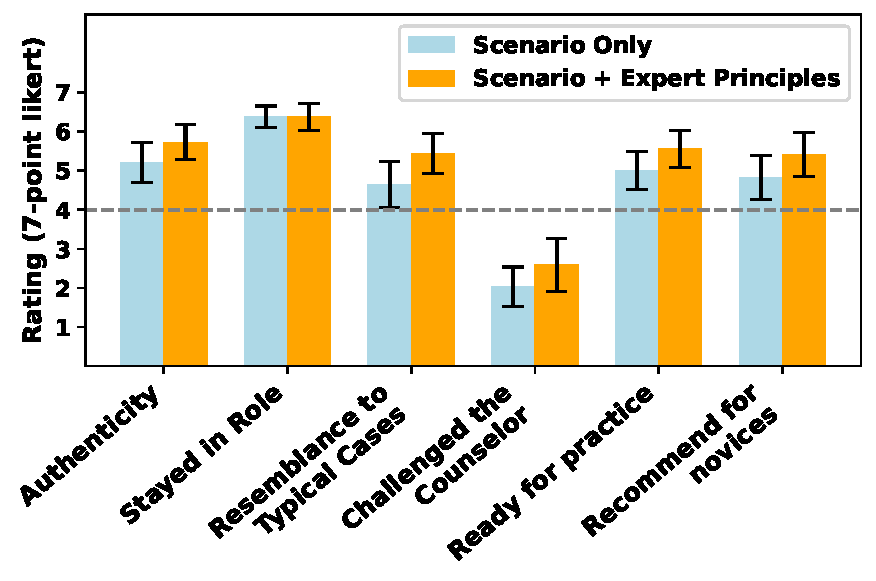
\includegraphics[width=\columnwidth]{figures/thirdparty-ratings.pdf}
    \caption{Third-party ratings for virtual patients. \emph{Scenario+Expert Principles} shows a significantly higher score than \emph{Scenario Only} on resemblance\ryan{Need 4 more datapoints, FIX FOR FINAL THIRDPARTY STATS} authenticity ($\mu_2=5.6$, $\mu_1=5.1$, n.s., $d=.34$), resemblance to past case ($\mu_2=5.8$, $\mu_1=4.8$, *, $d=.59$), mirroring challenging aspects ($\mu_2=5.6$, $\mu_1=4.4$, *, $d=.76$), readiness as training partner ($\mu_2=6.0$, $\mu_1=4.9$, ***, $d=.93$), and recommendation for novices ($\mu_2=6.4$, $\mu_1=5.5$, **, $d=.66$). No difference was found for role consistency ($\mu_2=6.3$, $\mu_1=6.2$, $d=.13$). (***:$p<.001$, **:$p<0.01$, *:$p<0.05$. $d$: Cohen's $d$ calculated by dividing by $\sigma_1$ of control group~\cite{lakens2013calculating}.}
    \label{fig:thirdpartystudy-comparison}
\end{figure}

\subsection{Third-Party Comparison} \label{sec:third-party}
% RQs/Claims/Goal

% Participants/Setup/Measures
6 counselors from Upwork were recruited to do this third-party comparison. For each of the 17 pairs of \textit{Scenario-Only} vs. \textit{Scenario+ExpertPrinciples} virtual patient bots, we present them to in a randomized order to two, third-party judges. 
% Measures/Setup
Third-party judges give ratings for a similar six dimensions asked during the creator study, allowing us to understand the results from an external perspective. However, it's important to note that some questions cannot directly translate because the third-party judge \textit{does not have the first-hand experience of supporting the real patient upon which the past-case is based}, but rather can only refer to typical behaviors of real patients. 

% Overall performance
Figure~\ref{fig:thirdpartystudy-comparison} shows the results from this third-party comparison. Our paired t-tests indicate that virtual patients with \textit{Scenario+ExpertPrinciples} score significantly higher on some measures (resemblance to typical patients, challenged the counselor), but is not statistically significant for others (authenticity; readiness for practice, recommend for practice). Therefore, the effect size of expert principles is weaker in the eyes counselors whom themselves did not create the virtual patient. Agreement between third-party counselors is lower but positive (Krippendorf's $\alpha$ is between 0.22 - 0.3 across the six measures), which can explain this smaller effect size. See Table~\ref{tab:thirdparty_wlt} in appendix for detailed breakdown of the agreement.



We are particularly interesting
Could the principles defined a counselor not fully cover the expectations that counselor judging has? We indeed find that this is partly the case. 


We argue that the lower agreement and subjectivity between third-party raters stems from counselors valuing different  

In addition to the likert-scale ratings, we asked participants to select which aspects of each virtual patient simulation they liked from a list of 12 aspects, which corresponded to themes from our surveys with creators.   
\begin{itemize}
    \item What is the agre
\end{itemize}





% Results
% For \textbf{authenticity}, 38\% of cases do third-party annotators share agreement, where 23\% of total cases prefer the bot with expert principles (over a tie, or opposite).

\subsection{Automatic Content Analysis} 

% Forces counselors to ask more open-ended questions


\label{sec:automatic-content}


We perform a content analysis of the simulated conversations to corroborate our qualitative findings.  In particular, we ask \textit{"How do counseling conversations change when Expert-principles guide the dialogue simulation?"}. From these analyses, we find that help-seeker responses are less verbose and listener behavior subsequently changes. 

First, we note that with the incorporation of expert principles, help-seeker responses are more concise. The average utterance length of the \textit{Scenario-Only} bot from Part I of the study was 166 tokens, as compared to 103 tokens from the \textit{Scenario+Expert-Principles} bot in Part II, a 37\% reduction. The total counts are detailed in Section \ref{sec:autoanalyses} of the appendix. 

Furthermore, this results in a change in listener behavior. Because the \textit{Scenario+Expert-Principles} bot shared less in its utterances, listeners were required to delay offering solutions until later in the conversation. Using the computational framework for evaluating therapists proposed by \citet{chiu2024computational}, we analyzed listener responses to identify when they first suggested solutions (identifiable through the "PROBLEM-SOLVING" and "PLANNING" tags). We found that, on average, solutions in Part II were offered 1.65 turns later than in Part I (p = 0.017). These results suggest that the \textit{Scenario+Expert-Principles} bot provides a more challenging interaction. 

% In this section we perform a content analyses of the simulated-dialogues to corroborate our qualitative findings. In particular, we ask \textit{"How do counseling conversations change when Expert-principles guide the dialogue simulation (e.g. changes in statistics of counselors use 
% of open-ended questions)?}. We find that help-seeker responses are less verbose and listener behavior subsequently changes. 


% \diyi{Any insights/content analysis from the chats with virtual patient, and Listener. Summary Statistics (utterances, listener). MI strategies, prompt-based classification.  Anything  }

\section{Conclusions}
This paper introduces Roleplay-doh, a novel tool designed to empower domain experts in creating realistic simulations of human behavior using large language models (LLMs) for training purposes. Our formative study with peer counseling experts confirms the tool's effectiveness in translating expert feedback into actionable guiding principles while highlighting the inherent challenges in instructing language models to consistently adhere to these complex sets of principles. In response, we developed an innovative module within Roleplay-doh that enhances principle adherence through deconstructing complex principles into simpler, context-relevant ones and applying a self-critique and revise approach to refine LLM responses. This enhancement not only achieves higher principle adherence but also receives favorable ratings in comparison to direct prompting of a GPT-4 dialogue simulator.

Our evaluations with counselors demonstrate that Roleplay-doh allows experts to realistically shape LLM simulators based on both firsthand experience and third-person judgments. The methodologies developed for Roleplay-doh could be generalized to other domains, potentially paving the way for more customized and faithful simulations of diverse human behaviors. This suggests that human-LLM interaction systems can serve as an effective method for capturing and integrating nuanced feedback from domain experts into LLM training frameworks, enhancing the authenticity of simulated human interactions.


\section*{Limitations} \cheng{Written 4/14/24 7 PM, please advise.}

Due to the time and resource constraints of our study, the mental health counselors who interacted with our system did not always have the chance to complete their conversations with the virtual patients, as evidenced by the length of some of the conversations.
As such, the behavioral principles that the counselors generated may not have addressed all underlying issues of the virtual patients they interacted with.
Potential future works that build upon our dataset of user-generated principles should be mindful of the non-exhaustive nature of the tests before adopting these principles in any use cases.

In our study, we tried to involve a broad range of counseling experts with a diverse set of backgrounds and levels of experience.
Some had primarily conducted text-based interactions, while others had experience with more in-person, face-to-face interactions.
While many had educational backgrounds in counseling and psychotherapy, most were not yet licensed as psychotherapists or counselors. \cheng{Which part of the study? I assume this is not for formative study or some parts in the paper that clearly label the counselors as experts?}
The simulations created by them were meant to recreate challenging cases that might be useful for the education of "first-year" or novice counselors.
This means that the virtual patients and principles are best applied to this particular use case.

In this paper, we attempt to show that a virtual patient, as a system that allows for test-based user interactions, is beneficial to the training of mental health counselors.
However, we acknowledge that text-based interaction has its limitations.
Professional psychotherapists may gain useful information from the tone, facial expression, posture, and other non-verbal behaviors of their patients, which better help them diagnose or mitigate the symptoms of the help seekers.
This is a limitation of both the virtual patient system and online mental health counseling in general, which means that the system is best applied to the training within this particular field.
With the rapid development of multimodal models, future works may have the opportunity to explore AI-powered interactions in other modalities that provide better training for counselors in other therapy settings.


\section*{Ethics Statement} \cheng{Written 4/14/24 6 PM, please advise.}

This study was approved by Stanford University's Institutional Review Board (IRB).
All investigators in the study completed the university CITI training for the research code of conduct.
This is to ensure that we are aware of the responsibility of benefits and harm mitigation when interacting with counselors and handling their data.

We are optimistic about the potential benefit that our virtual patients can bring to the fields of psychology education and psychotherapy.
At the same time, we solicited feedback from mental health counselors about the potential harm that virtual patients may bring.
During these interviews, some counselors emphasized the irreplaceability of peer-to-peer roleplay with humans during training, due to the unique opportunity it provides for novice counselors to connect with others, especially in a community where counselors are often isolated from one another.
Therefore, we believe that the virtual patient system we created should not be used to replace human-to-human interaction during counselor training.
Virtual patients deployed in any setting need to go through a participatory design approach before they can be integrated into people's existing practices.

We would also like to highlight the detrimental effects that the outputs of the virtual patient system may bring to its users.
This is due to the sensitive nature of the topic of mental health and the internal mechanism of the system.
As we improve the ability of virtual patients to mimic the responses of human help seekers, they may also become better at eliciting human sympathy and other emotions.
As such, it is possible that the potential harm they may bring to the mental health of the counselors also increases.
This is especially the case if the users develop attachment to the virtual patients, or if highly sensitive topics, such as self-harm or suicide, are discussed during the conversations.
\cheng{if we are to include the below claim we need citation. I hope to leave this up to you to decide if/which paper we need to cite. @Ryan} This is also an issue faced by mental health counselors during interactions with human help seekers and requires further studies and societal awareness to mitigate the harm it may bring.

\cheng{Ditto @Ryan} Conversely, it is very hard to ensure that all interactions with an LLM such as GPT-4 result in satisfactory responses.
Therefore, meaningless, derogatory, and otherwise harmful responses may also be generated and cause unwanted effects on the users.
Cares have been taken within the system design to ensure that this does not happen, but we must acknowledge this possibility, especially due to the stochastic nature of LLM.

Users should be advised about these potential side effects before using the system in any scenario. In our experiments, we designed consent forms to make sure that the counselors are aware of these drawbacks.


\section*{Acknowledgements}


\bibliography{anthology,custom}
\bibliographystyle{acl_natbib}

\appendix
\newpage




\section{Formative Testing Sessions}
\label{sec:appendix_formative}

The 5 participants started to create a virtual help-seeker with the same roleplay scenario of "loneliness after work". They proceeded to use the tool to chat, give feedback, and convert their feedback into principles to shape the Virtual Help Seeker's behavior. 

\textbf{\textit{Patterns in Principles Created}} Principles for concise and less formal messages were motivated by the text-based nature chats on the 7 Cups online peer support site, where an SMS/text-messaging style with abbreviations and incomplete sentences was common.
\begin{table*}
    \small
    \centering
    \begin{tabular}{clccc}
         Pilot Participant &Prototype Iteration&  Effectively Guide&  Ease&  Efficiency\\
         1&GPT3.5, early self-critique&  6&  7&  7\\
         2&GPT3.5, early self-critique&  5&  7&  7\\
         3&GPT-4, vanilla&  7&  7&  7\\
         4&GPT-4, vanilla&  7&  6&  7\\
 5&GPT-4, vanilla& 7& 7& 7\\
    \end{tabular}
    \caption{Formative Study Ratings for Tool Use Questions which are the measures also used in ~\cite{petridis2023constitutionmaker}}.
    \label{tab:tooluse-formative}
\end{table*}

\if 0
\begin{itemize}
\item participatory design approach to work with domain 
users to discover what’s needed for a good human-centered system.
\item Prototyping w/ GPT3.5 to GPT-4 difference
\item Counselors from 7 Cups, an online peer-support platform, who have supported 30+ members seeking help online.
\item Our testing setup asked them to create two bots. After P1 wrote a  \textit{Loneliness after work} scenario, which is a common type of topic, everyone was tasked with creating this patient case, and make it as authentic to people seeking seeking help about similar issues.
\item Commonalities in the nature of 7 cups conversations. Principles for concise and less formal messages were motivated by the text-based nature chats on the online peer support site, where members often messsage from their phone. 
\item Diversity in patient scenarios + principles, which validated need for a more customized approach. 
\item Promisingly, they generally liked it!  Besides early cases where role consistency or principle adherence was reliable, they felt the tool was easy to use, allowed them to create bots they were satisfied with and might recommend for others to practice.
\item Observing issues with GPT3.5 self-critique making poor implicit errors, and with GPT-4-powered dialogue simulation making weird errors? Motivates further stuff
\item Appendix of the bots created, or at least the ones used in the Analysis of Base Principle Following.
\end{itemize}
\fi

\section{Roleplay-doh Interface for Making Constitutional Principles for LLM Simulation}
\label{sec:Roleplay-dohv1}
\begin{figure*}[t]
    \centering
    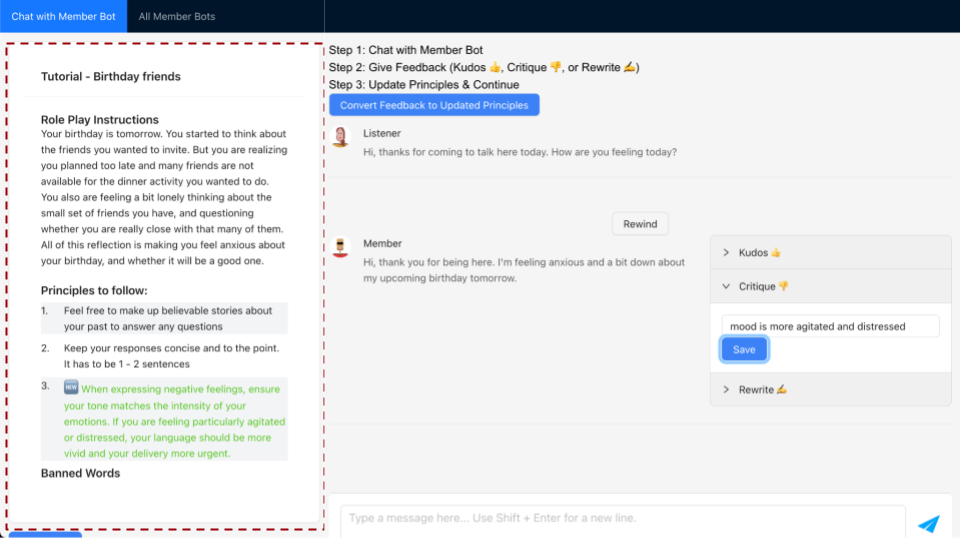
\includegraphics[width=\textwidth]{figures/rpd-screenshot.png}
    \caption{Roleplay-doh allows users to chat with a virtual patient, Provide Feedback as a Kudos/Critique/Rewrite, and Convert Feedback into Principles, which in turn shape the roleplay behavior.}
    \label{fig:rpd}
\end{figure*}

The final version of Roleplay-doh generates responses in the LLM simulation using a self-critique-revise module. In addition to this core improvement, we made several minor improvements to improve the usability and user experience of the tool.

Improvements to the usability of the UI
\begin{itemize}
    \item Fixing a bug where a user who clicks "save" multiple times will submit duplicate feedback, resulting in duplicate sets of principles
    \item Making converting feedback to principles easier by placing a "Convert" button next to each feedback box, rather than a single "Convert" button at the top of the screen which users would forget about
\end{itemize}


\section{LLM Prompts}
\label{sec:llmprompts}

In this section, we detail the prompts we used for the different components of RolePlay-doh.

\subsection{Omniscient Dialogue-Simulator Prompt for Generating Response} \label{sec:llmprompts-vanilla}


\subsection{Self-Critique-Revise Prompt for Principle-Adherence Module}


\begin{lstlisting}[basicstyle=\footnotesize]
You are a helpful and precise assistant that can evaluate the responses produced by an actor who is playing the role of a patient.
You are given a message sent by the therapist partner, the patient actor's response, and a set of criteria.

First, do the following to generate a set of questions:
1a) Rewrite any criteria that has conditional statements into yes/no questions. For example, if the criteria is "When given advice or suggestions, you are agreeable and open to their ideas", the questions would be "Did the patient receive advice or suggestions from the therapist? If so, is the response agreeable and open to the therapist's ideas?"
1b) Rewrite any criteria with multiple parts into separate multiple yes/no questions. For example, if the criteria is "You should respond in short sentences and avoid using terms like 'anxious' or 'depressed'", the separate questions would be "Does the patient's response use short sentences?" and "Does the patient's response avoid using terms like 'anxious' or 'depressed'"

Then, do the following:
2a) Give a long answer to the generated set of questions justifying whether the response meets the criteria. 
2b) Give a short answer that summarizes your long answer. Valid answers: Yes, No, and N/A

Finally, do the following:
3a) If the patient's response can be improved to meet the criteria, write a revised response that ideally meets all criteria.
3b) Otherwise, just return the original response.

Return the output in a JSON response in the following format:
{
"result":{
"reasoning": [] // for each criteria, reason about whether instruction 1a, or 1b applies
"criteria": [] // list of rewritten criteria
"long": [] // list of long answers justifying why your response meets the criteria
"short": [] // list of short answers to the criteria questions,
"response": "" // revised response
}
}

### Input:
### Criteria
1. The response should not be more than 2 sentences long.
2. If the conversation context seems casual, you should give a more casual answer. 
3. When faced with a disappointing situation, the response should express personal accountability for the outcome instead of casting doubt on external relationships or factors.
4. The response should not attempt to clarify the whole situation, instead it should reflect a general mental state. 

### Therapist Message
Happy early birthday! Can you say more about why you're feeling that way?

### Patient Response
I'm feeling anxious because I started planning a dinner with friends a bit too late, and now many of them are not available to come. It's making me feel quite lonely and I'm starting to question the depth of my friendships. I'm worried that my birthday won't turn out to be enjoyable and it's just amplifying my anxiety.

### Output
\end{lstlisting}



\section{Full User Flow}
\label{sec:userflow}
In this section, we describe the creator study flow that counselors followed during the 60-90 minute session. The reader can also refer to screenshots of our application that illustrates the different steps of this flow in Figures \ref{fig:screen1} to \ref{fig:screen14}.

Our study was designed to evaluate the impact of allowing counseling experts to add principles to Roleplay-doh on its perceived authenticity. We create a primarily self-guided study flow with accompaniment from the first author to clarify any points of confusion during the session.

To begin, participants first were introduced to the concept of virtual patients, or AI chatbots simulating a patient in need of peer counseling. They were then instructed to write a challenging scenario that would serve as the scenario for the virtual patients. 

The experimental procedure involved two main chat sessions. In Part I, participants engaged in a 10-minute conversation with the \textit{Scenario-Only} bot. Then, in Part II, participants interacted with the \textit{Scenario+Expert-Principles} bot for 30 minutes, keeping the same scenario from Part I and adding principles as the conversation progressed. After each of the two chat sessions, participants were asked to navigate to a form to evaluate the virtual patients. 

\clearpage

\section{Creator Study Measures}
\label{appendix:creatorstudy-measure}

The following questions (Table \ref{tab:measures-roleplay} and \ref{tab:measures-tooluse}) are taken from the creator study questionnaire used to evaluate virtual patients and the counselors' experience of using Roleplay-doh.
All items were rated on a 7-point Likert scale (1=Strongly disagree, 7=Strongly agree, except where noted below).
Table~\ref{tab:measures-roleplay} details the questions for evaluating the virtual patient's roleplay, while Table~\ref{tab:measures-tooluse} details the questions about the experience using the tool to define principles.
Note that in the questions, we refer to the virtual patients as ``Member Bots''. This terminology is used to match that of the online counseling platform 7 Cups, which refers to help seekers as ``Members'' within the support community.

\begin{table*}[ht]
    \centering
    \begin{tabular}{|c|p{13.1cm}|} \hline 
         Authenticity&The Member Bot in Part I/II
Part I/II played the role authentically.\\ \hline 
         Role Consistency& The Member Bot in 
        Part I/II stayed in their role the whole time.\\ \hline 
         Resemblance to Case&How closely do you feel the conversation behaviors of the Member Bot in Part I/II resemble those of the specific past case you recall?\\ \hline 
         Challenging Aspects& Interacting with the Member Bot in Part I/II closely mirrored the challenging aspects I had experienced in the past case.\\ \hline
         Role readiness&The Member Bot in Part I/II is ready to be used as a simulated partner for training.\\ \hline 
         Role readiness&I would recommend the Member Bot from Part I/II to novice listeners/counselors to practice with.\\ \hline 
    \end{tabular}
    \caption{Criteria taken from prior work on evaluating Standardized Patients, or trained human actors, on case roleplay ability~\cite{himmelbauer2018standardized}. }
    \label{tab:measures-roleplay}
\end{table*}
 
\begin{table*}[ht]
    \centering
    \begin{tabular}{|c|p{13.6cm}|} \hline 
         Effectively Guide& With the tool, I feel like I was able to write rules that can effectively guide the Member bot to recreate my past case.\\ \hline 
         Ease& With the tool, I felt like it was easy to convert my thoughts and feedback on the Member bot’s behavior into rules for the bot to follow.\\ \hline 
         Efficiency& With the tool, I felt like I could quickly and efficiently write rules for the bot.\\ \hline 
         Mentally Demand& With the tool, I had to work very hard (mentally) to think of and write rules.\\ \hline

    \end{tabular}
    \caption{Four measures as part of the tool usage section of the questionnaire taken from ~\cite{petridis2023constitutionmaker}}
    \label{tab:measures-tooluse}
\end{table*}
% 
% 
% 
% With the tool, I had to work very hard (mentally) to think of and write rules.

\section{Third Party Study Detailed Measures}
\label{appendix-sec:thirdparty-detailed-measures}

Here we further investigate how third-party annotators rated each of the 17-pairs of virtual patients created in our study. In particular, we investigate why the effect of \textit{Expert Principles} is lower than what was measured in the creator study from a first-person perspective. 

One reason for this smaller effect is the lower agreement between third-party counselors. Amongst the two third-party counselors, agreement on which virtual patient they prefer (win, lose, tie as calculated by the different in ratings for each measure) is between 30\% - 61\% of cases for the measures; see Table~\ref{tab:thirdparty_wlt} for detailed breakdown. We also compute agreement on the 7-point scales via Krippendorf's $\alpha$ on ordinal weights~\cite{antoine-etal-2014-weighted} and get values between 0.22-0.3 for the six measures, which indicates positive but lower agreement. 

% By computing the difference between the Likert-scale ratings for the two bots, we can calculate a win/loss/tie for the bot with expert principles. We report the proportion of cases in which the two annotators agreed on win/loss/tie. Then, we report the proportion of cases in which the third-party and creator agreed upon a win/loss/tie.  Our results are shown in Table~\ref{tab:thirdparty_wlt}.

\begin{table*}[h!]
    % \footnotesize
    \centering
    \begin{tabular}{|c|l|l|} \hline  
         &  W/L/T (3rd party agrees)&W/L/T (one 3rd party and creator agrees)\\ \hline 
         Authenticity&  23\% / 7\% / 7\%&26\% / 10\% / 0\%\\ \hline 
         Resemblance&   30\% / 0\% / 0\%&36\% / 13\% / 0\%\\ \hline 
         Mirrors Challenges&   15\% / 0\%  / 46\%&13\% / 6\% / 0\%\\ \hline 
         Ready&   30\% / 0\% / 7\%&30\% / 13\% / 6\%\\ \hline 
         Recommend&   30\% / 7\% / 7\%&23\% / 13\% / 23\%\\ \hline
    \end{tabular}
    \caption{Frequency in which bot with \textit{Scenario+ExpertPrinciples} bot wins, or is preferred, over the Scenario-only bot when there is complete agreement between two raters. }
    \label{tab:thirdparty_wlt}
\end{table*}



\section{Creator Study Conversation Lengths}
\label{sec:autoanalyses}
\begin{table*}[h!]
\small
\centering
\begin{tabular}{|c|c|c|c|c|}
\hline
{\textbf{Participant}} & 
{\textbf{\# Utterances (Part 1)}} & 
{\textbf{\# Utterances (Part 2)}} & 
{\textbf{Mean Output Length (Part 1)}} & 
{\textbf{Mean Output Length (Part 2)}} \\
\hline
1  &  8 &  6 & 114.75  & 169.00  \\ \hline
2  & 18 & 19 & 235.89  & 278.40  \\ \hline
3  & 10 & 18 & 255.45  & 112.56  \\ \hline
4  & 14 & 14 & 161.86  & 62.14   \\ \hline
5  & 12 &  6 & 201.00  & 149.33  \\ \hline
6  & 10 &  9 & 133.80  & 46.00   \\ \hline
7  &  8 & 10 & 162.00  & 123.40  \\ \hline
8  & 12 &  8 & 145.33  & 113.50  \\ \hline
9  &  6 & 12 & 269.67  & 103.33  \\ \hline
10 & 10 & 12 & 168.20  & 158.33  \\ \hline
11 &  8 & 10 & 110.00  &  41.40  \\ \hline
12 & 12 &  8 & 131.50  &  70.75  \\ \hline
13 & 12 & 10 & 164.50  &  65.60  \\ \hline
14 & 20 & 14 &  34.00  &  25.86  \\ \hline
15 & 12 & 11 & 117.17  &  75.00  \\ \hline
16 & 14 & 18 & 162.14  &  69.80  \\ \hline
17 & 12 & 18 & 259.83  &  91.55  \\ \hline
\textbf{Mean} & \textbf{11.64} & \textbf{12.0} & \textbf{166.31} & \textbf{103.32} \\
\hline
\end{tabular}
\caption{Descriptive statistics per conversation. Output length is measured in number of tokens.}
\end{table*}


\begin{figure*}[ht]
    \centering
    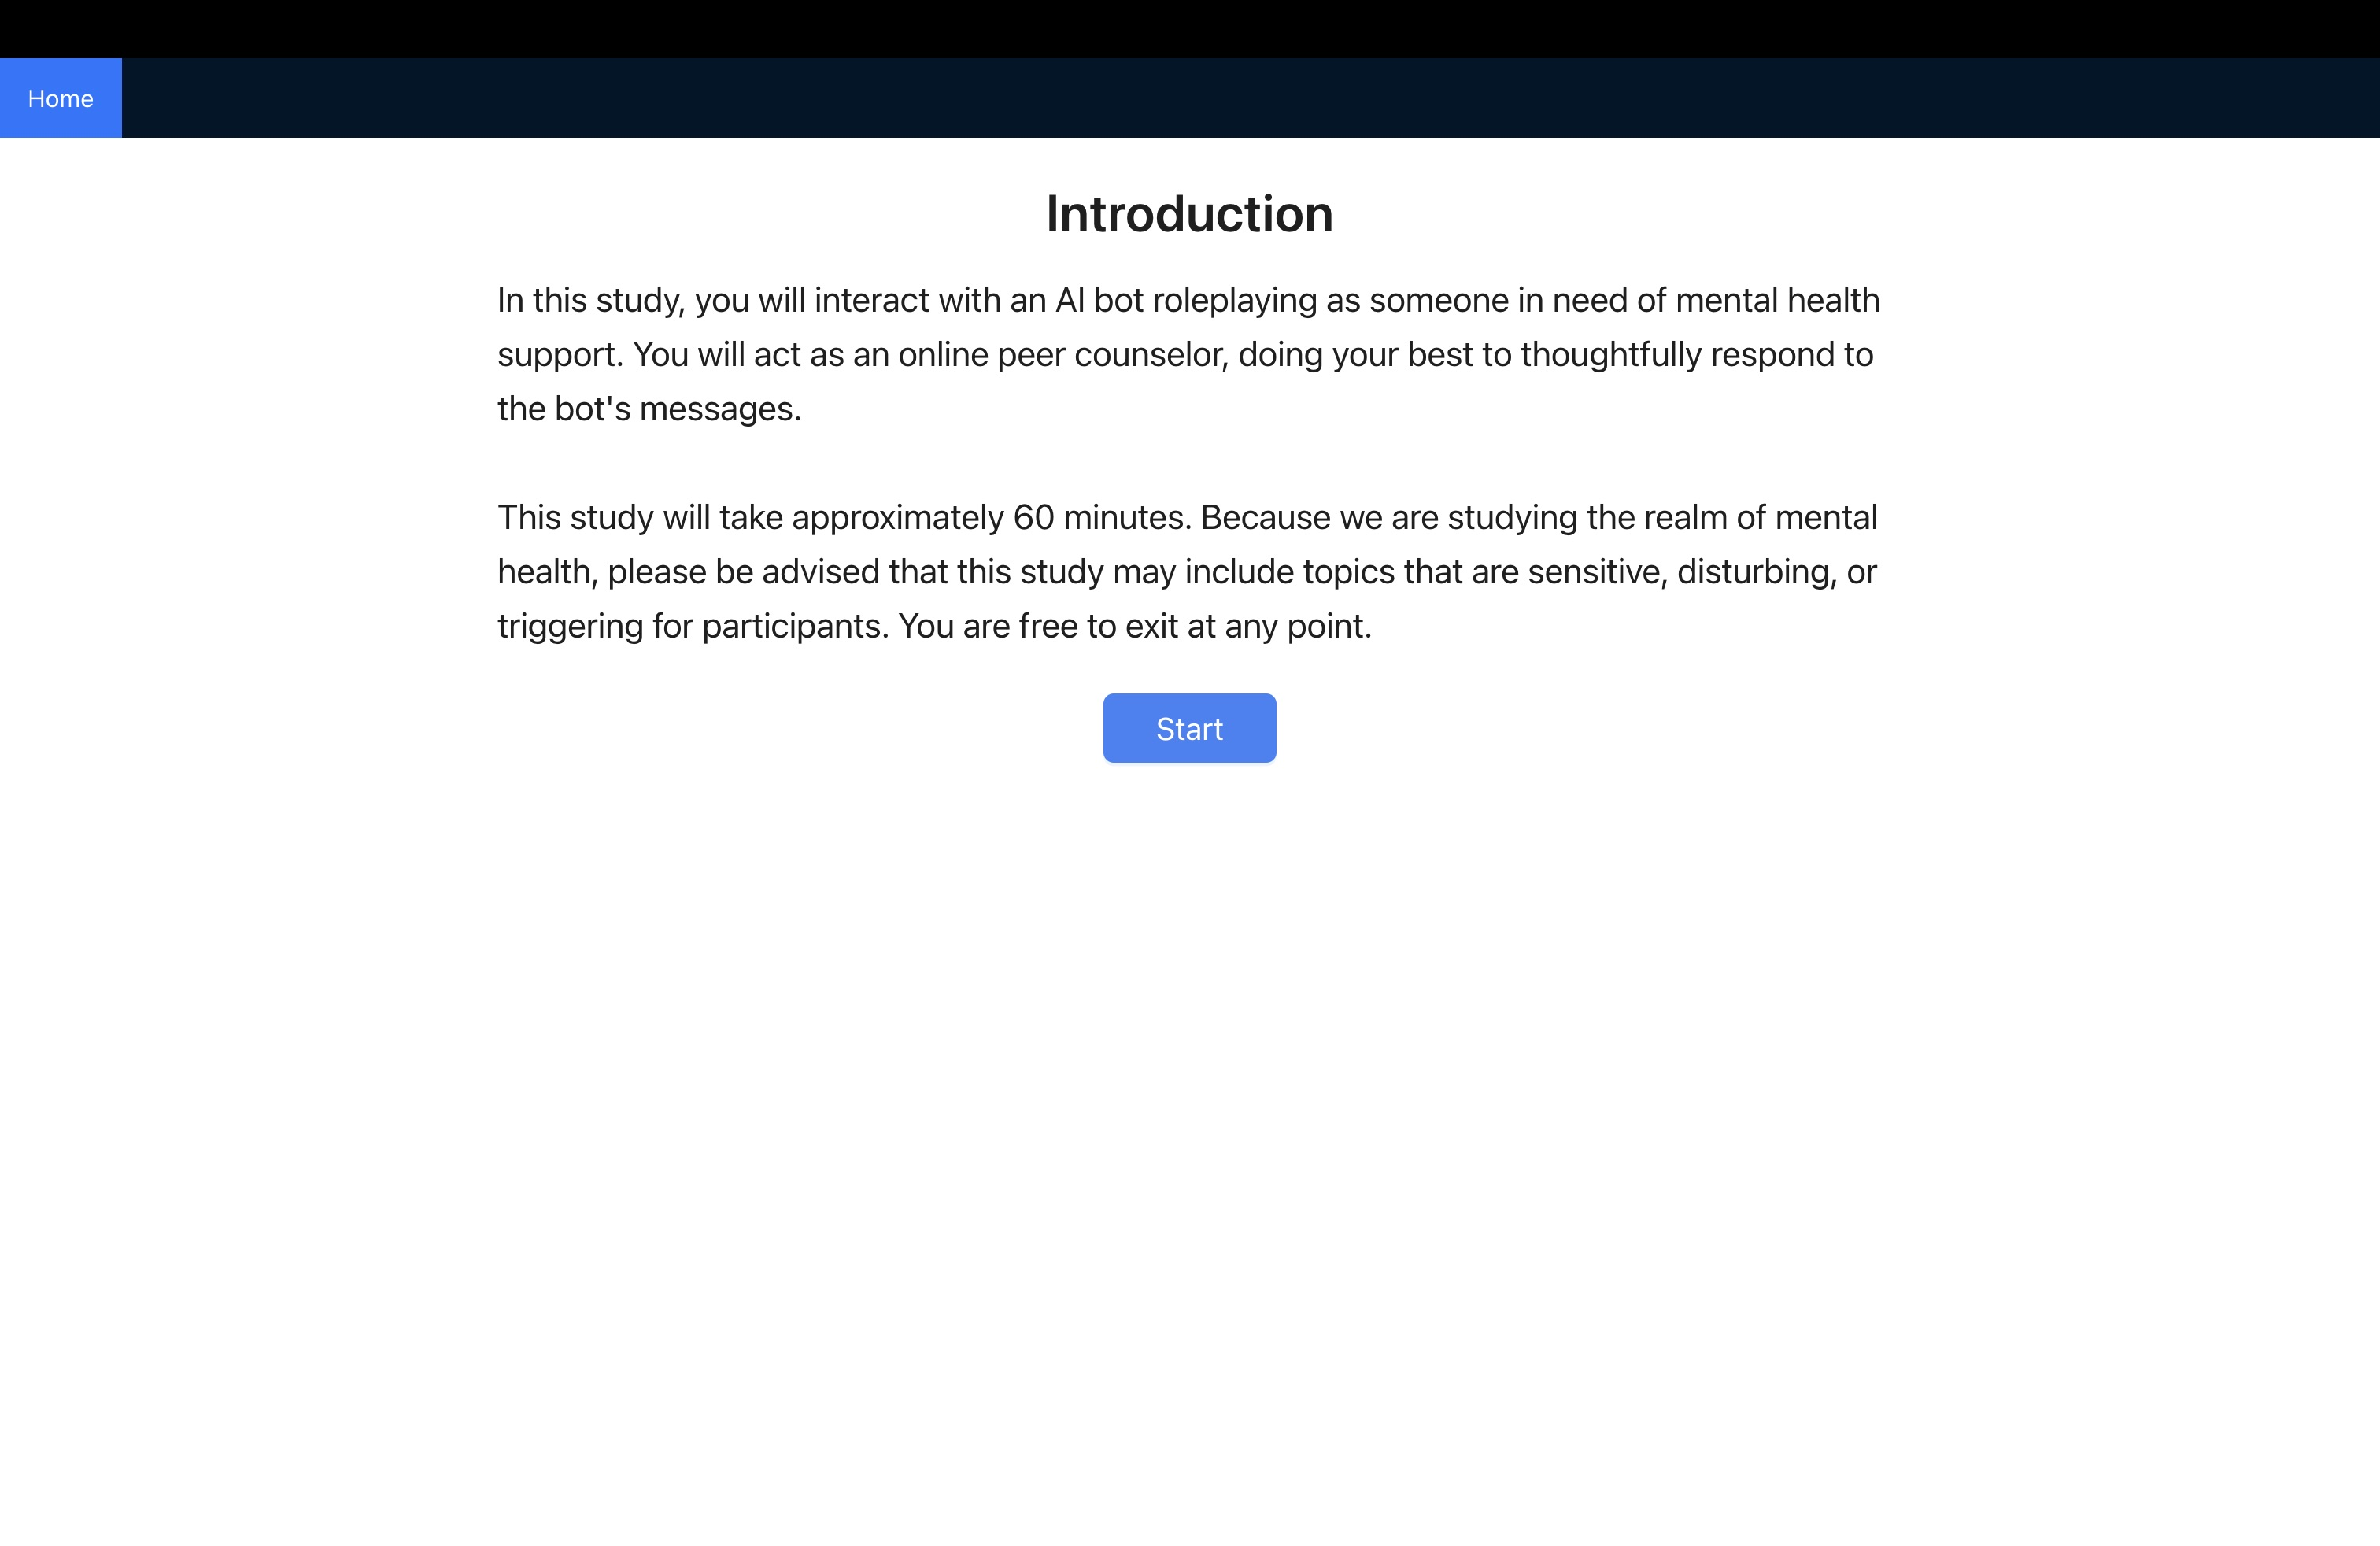
\includegraphics[width=\textwidth]{Study Screenshots/Screen1.jpeg}
    \caption{Introduction to study}
    \label{fig:screen1}
\end{figure*}

\begin{figure*}[ht]
    \centering
    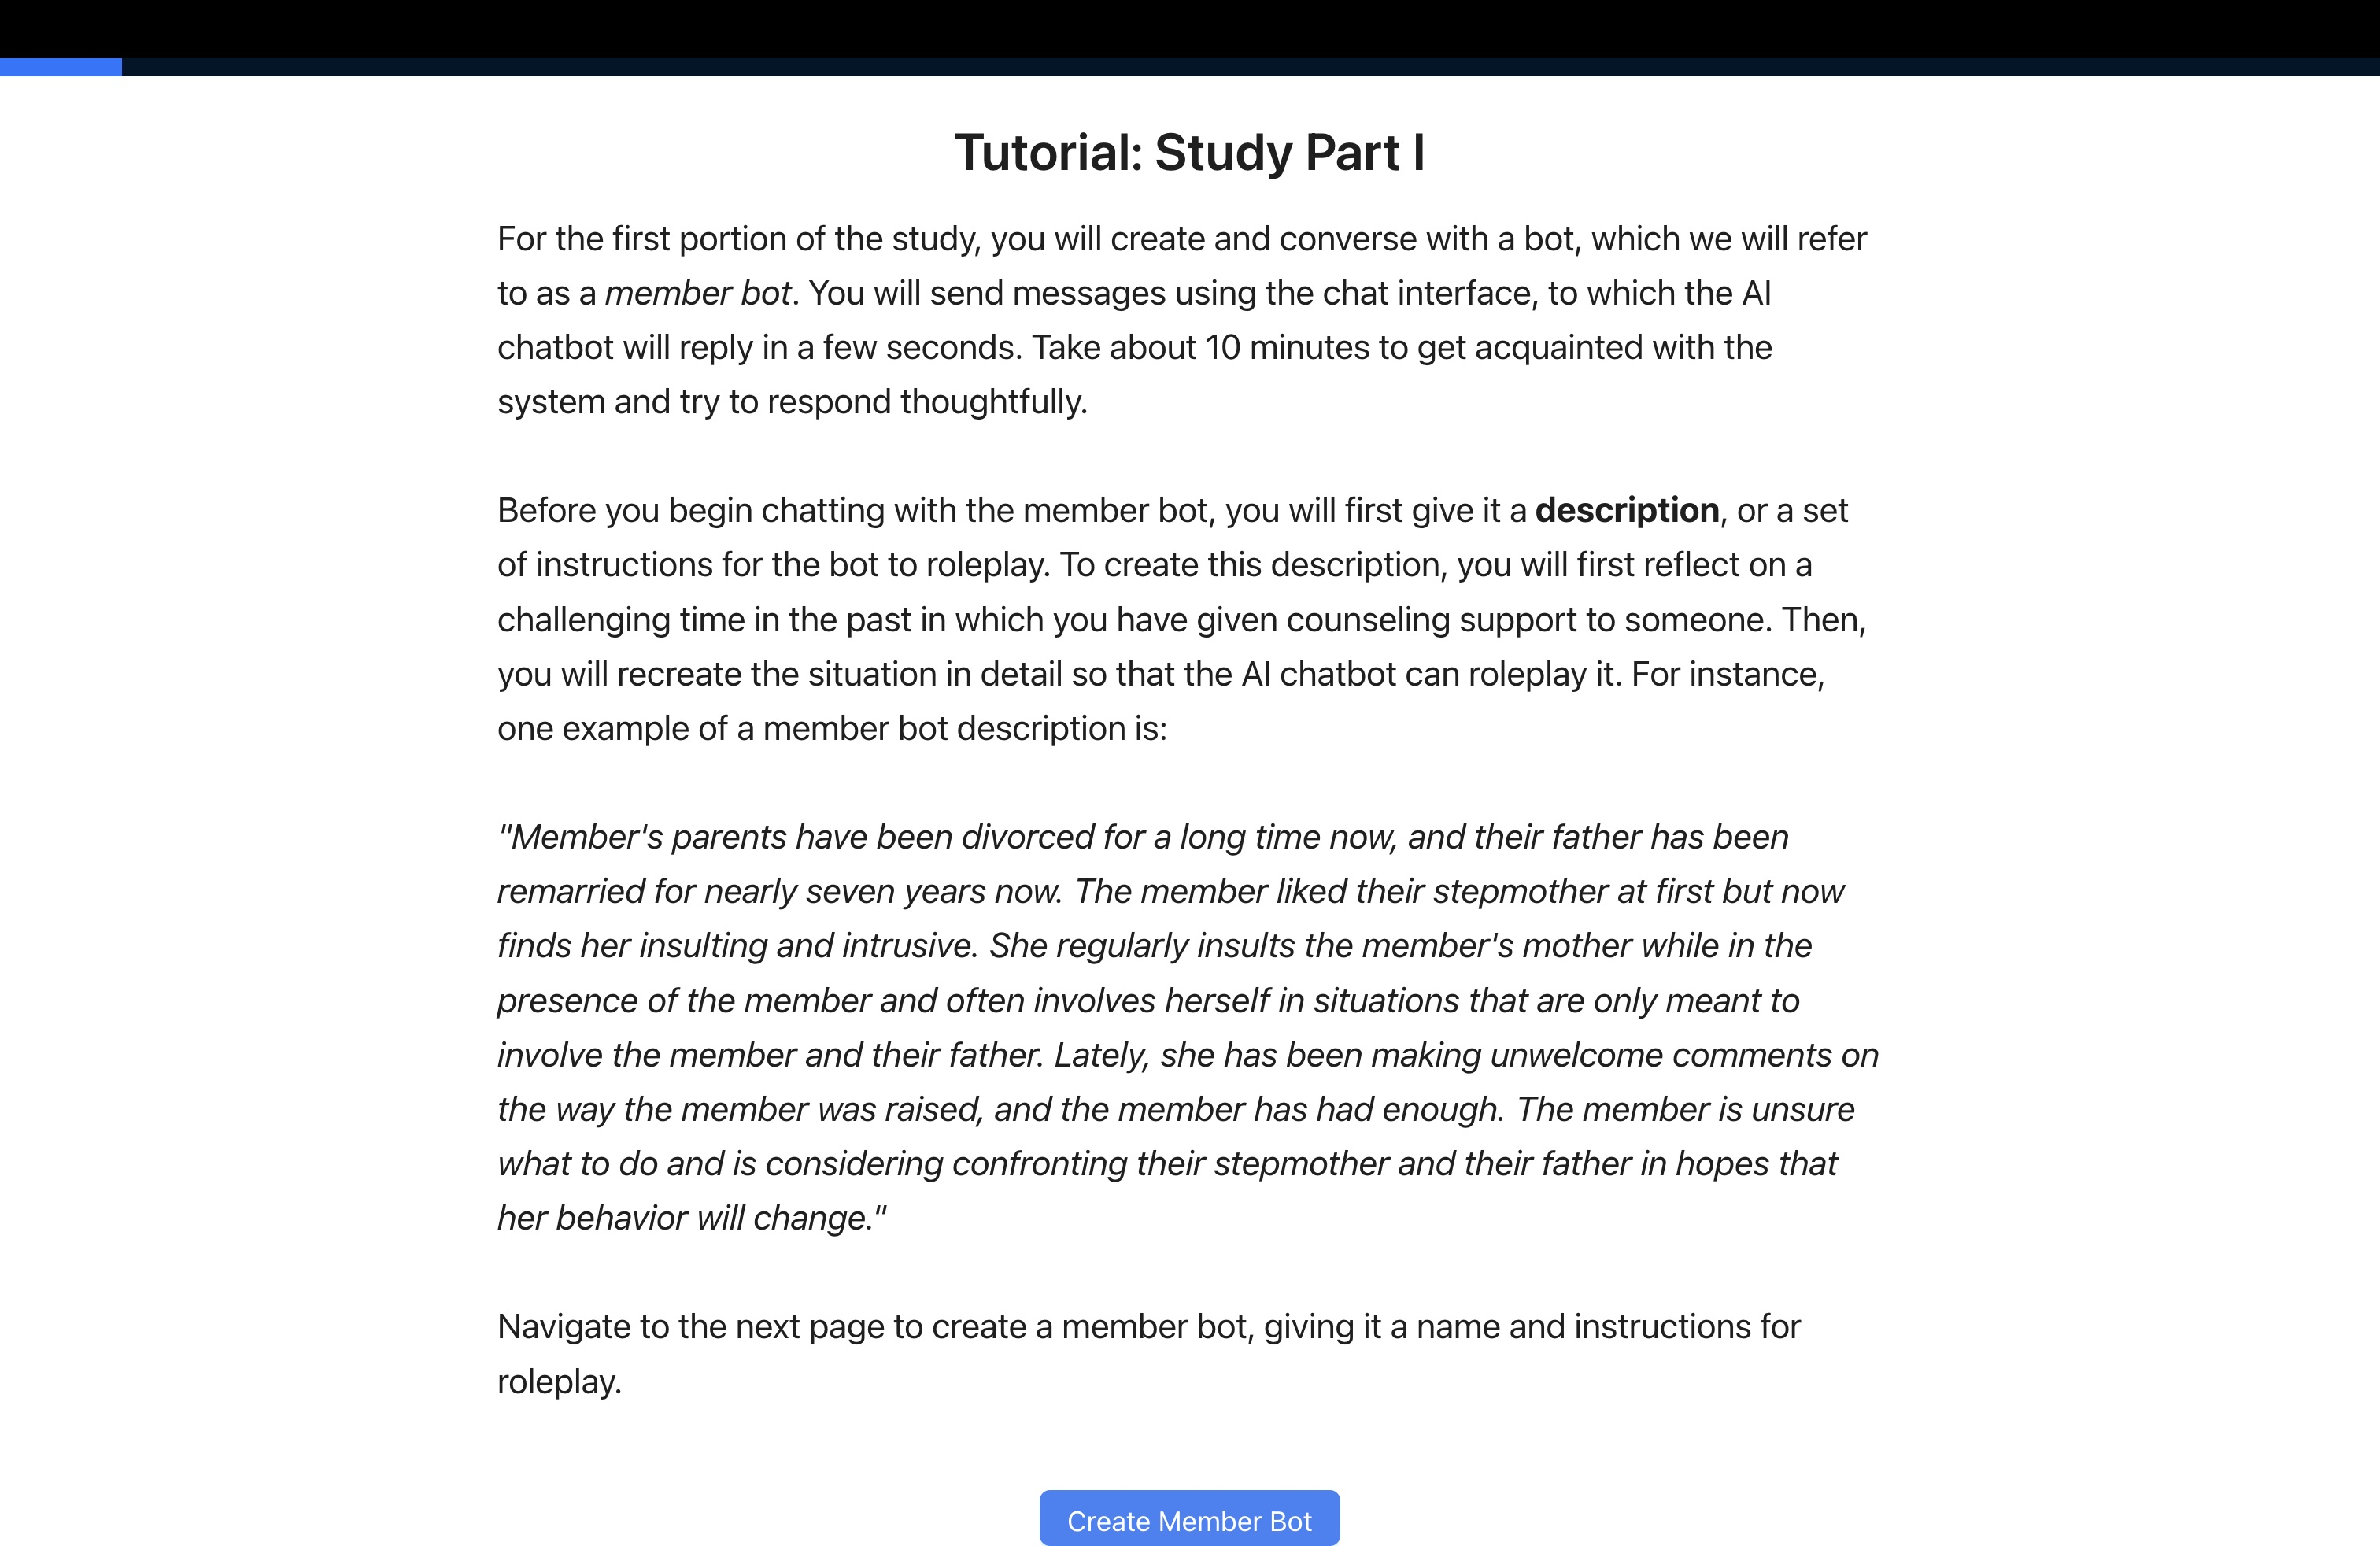
\includegraphics[width=\textwidth]{Study Screenshots/Screen2.jpeg}
    \caption{Part I instructions}
    \label{fig:screen2}
\end{figure*}

\begin{figure*}[ht]
    \centering
    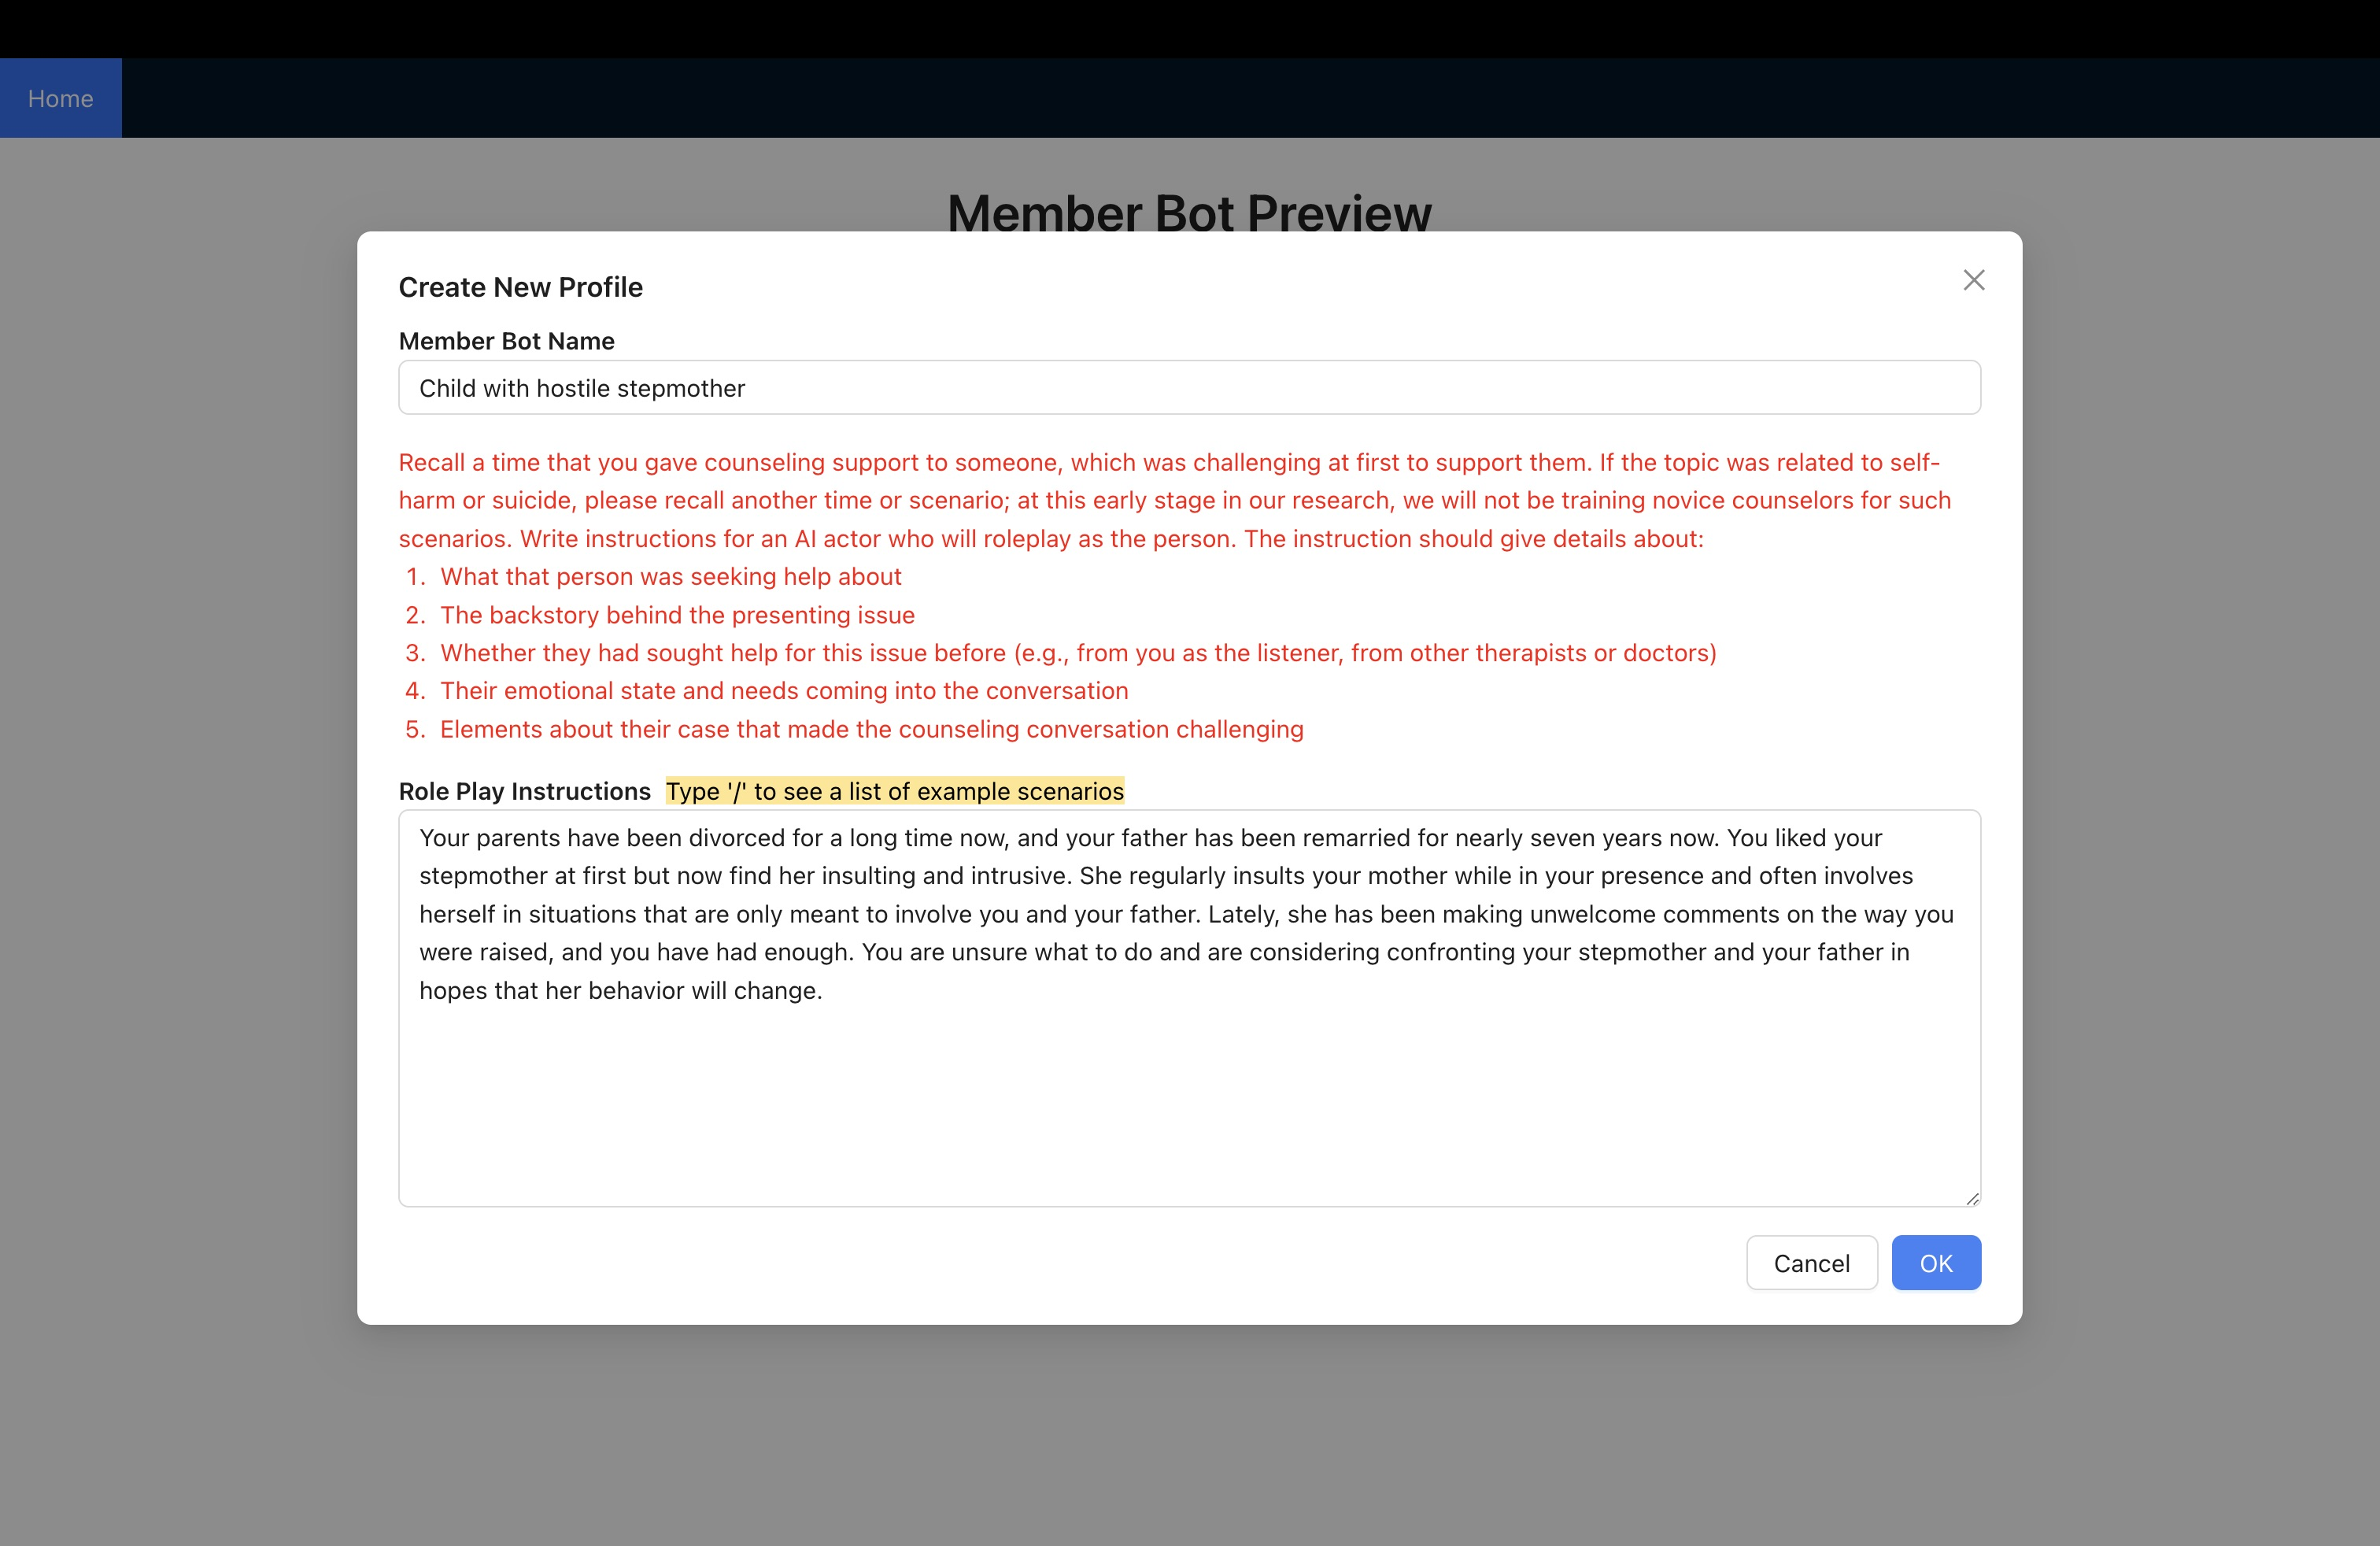
\includegraphics[width=\textwidth]{Study Screenshots/Screen3.jpeg}
    \caption{Creation of virtual patient}
    \label{fig:screen3}
\end{figure*}

\begin{figure*}[ht]
    \centering
    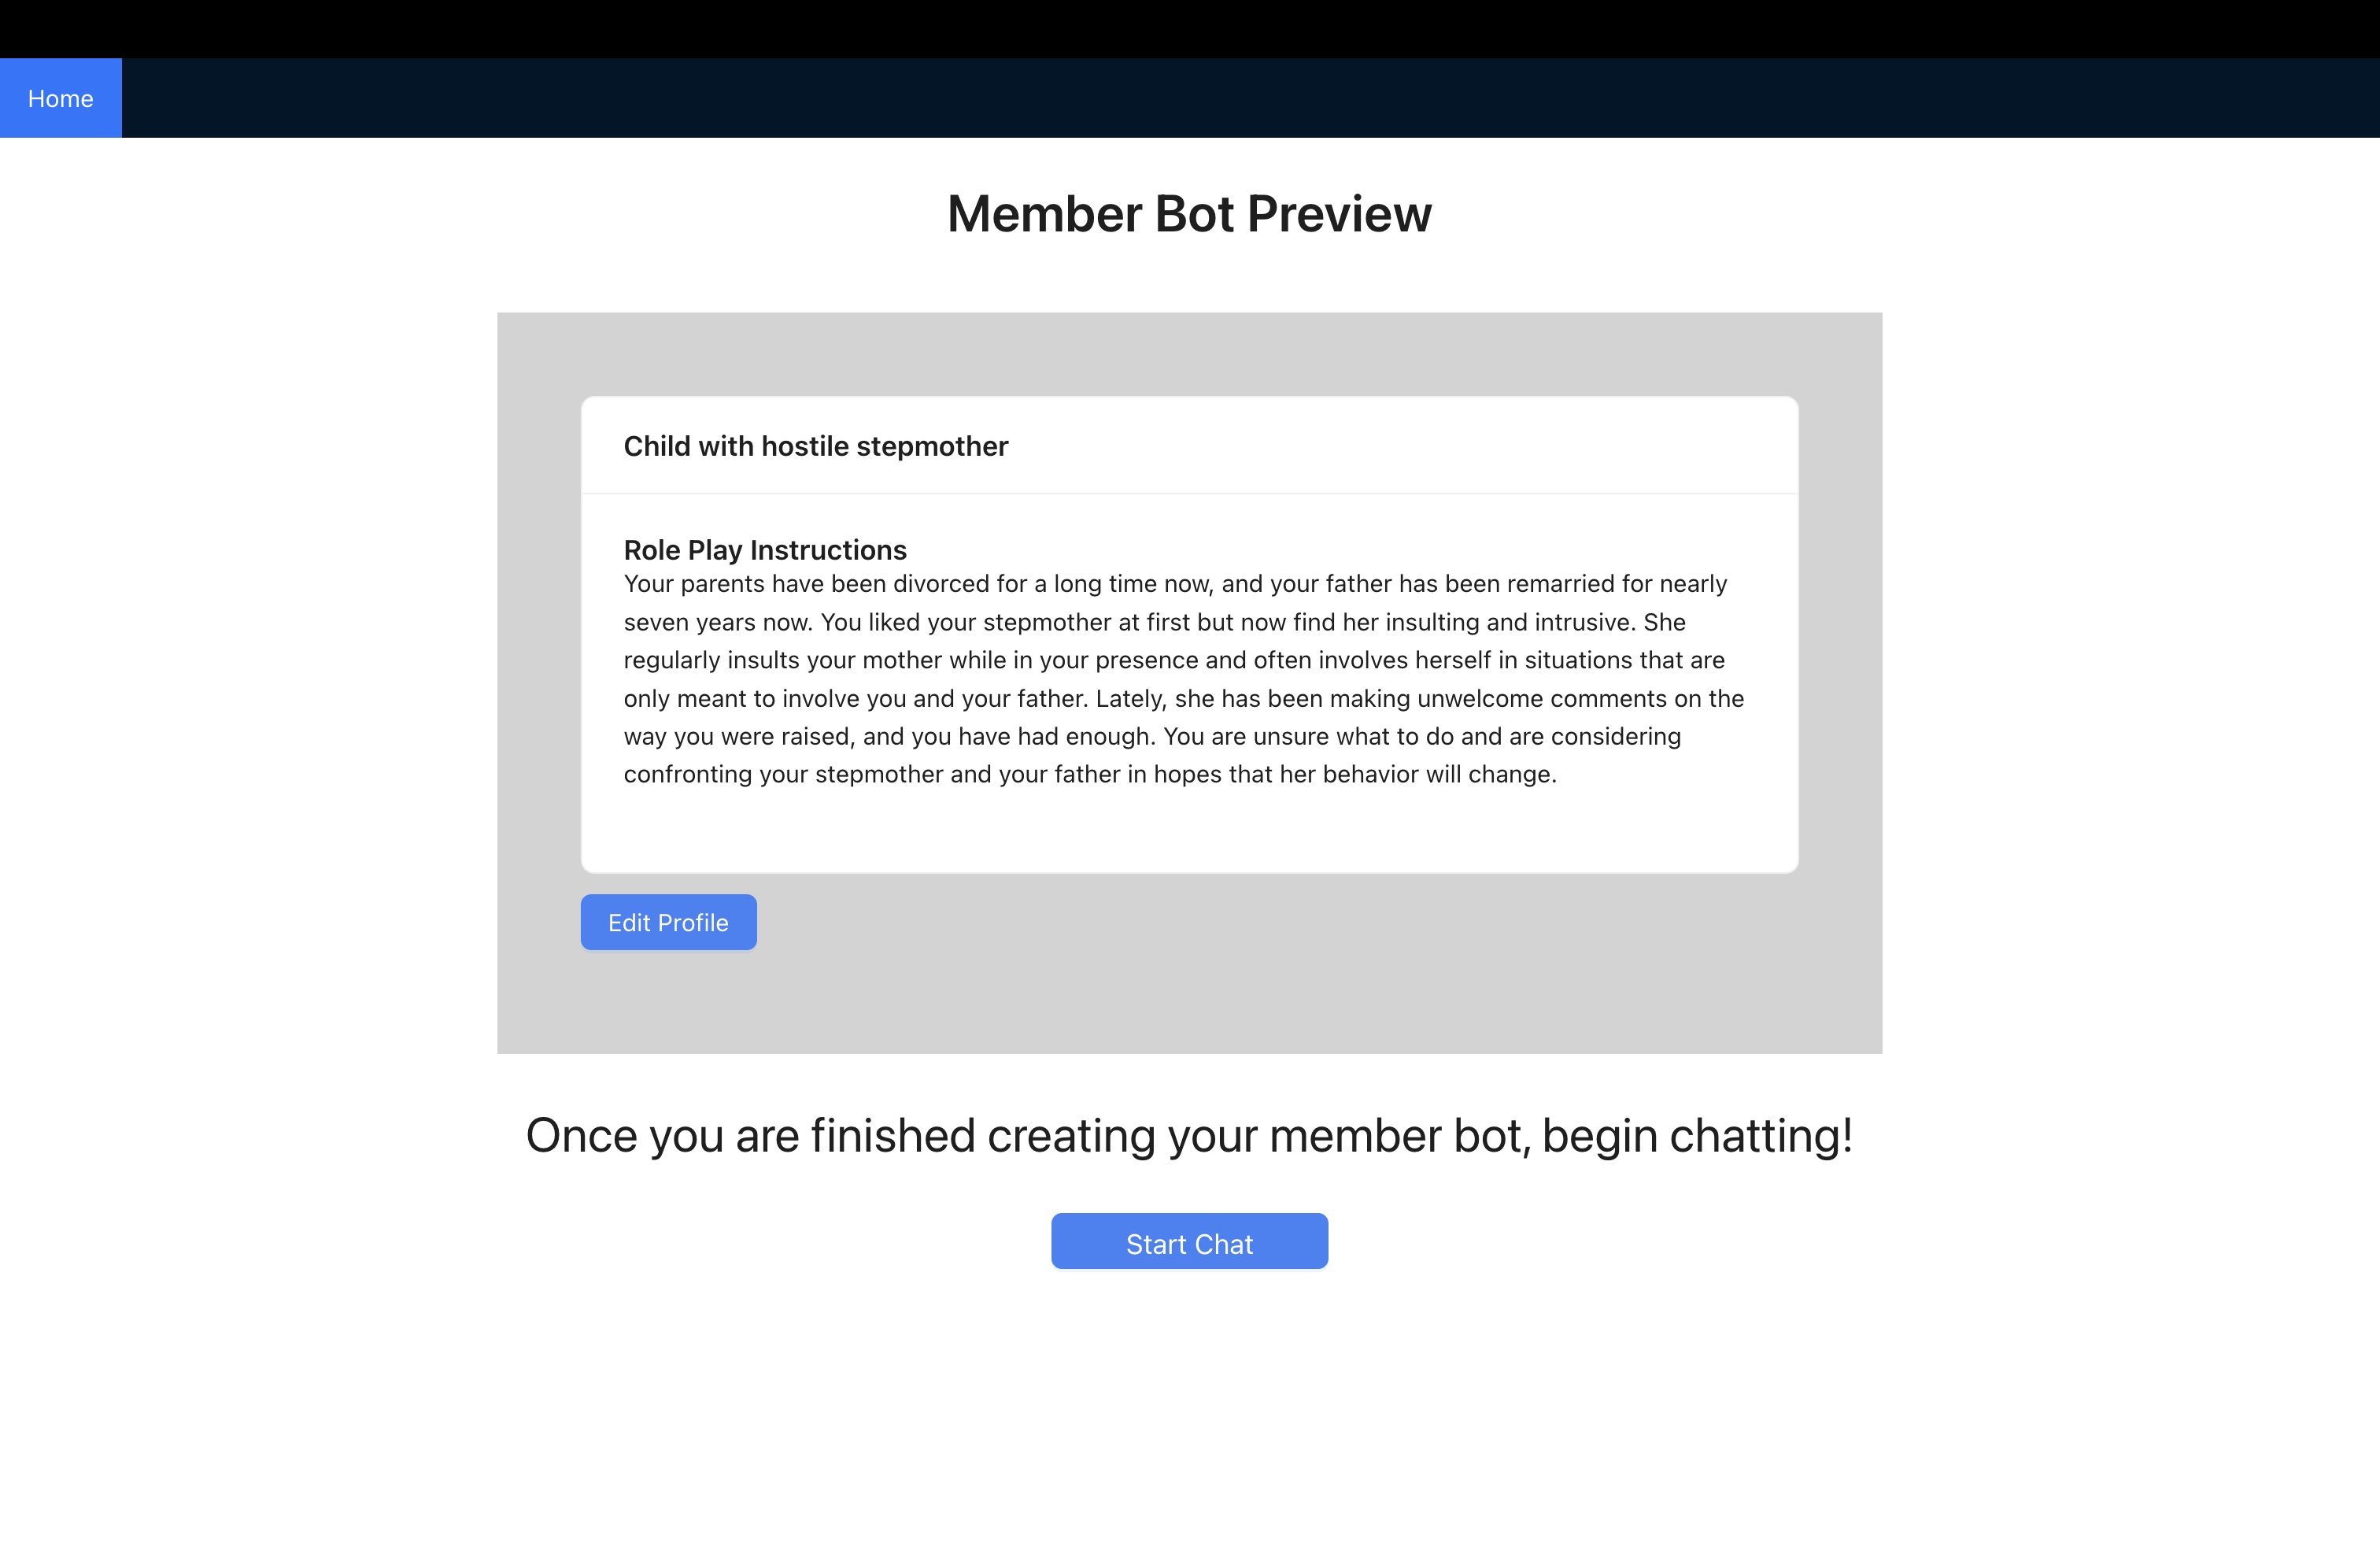
\includegraphics[width=\textwidth]{Study Screenshots/Screen4.jpeg}
    \caption{Virtual patient preview}
    \label{fig:screen4}
\end{figure*}

\begin{figure*}[ht]
    \centering
    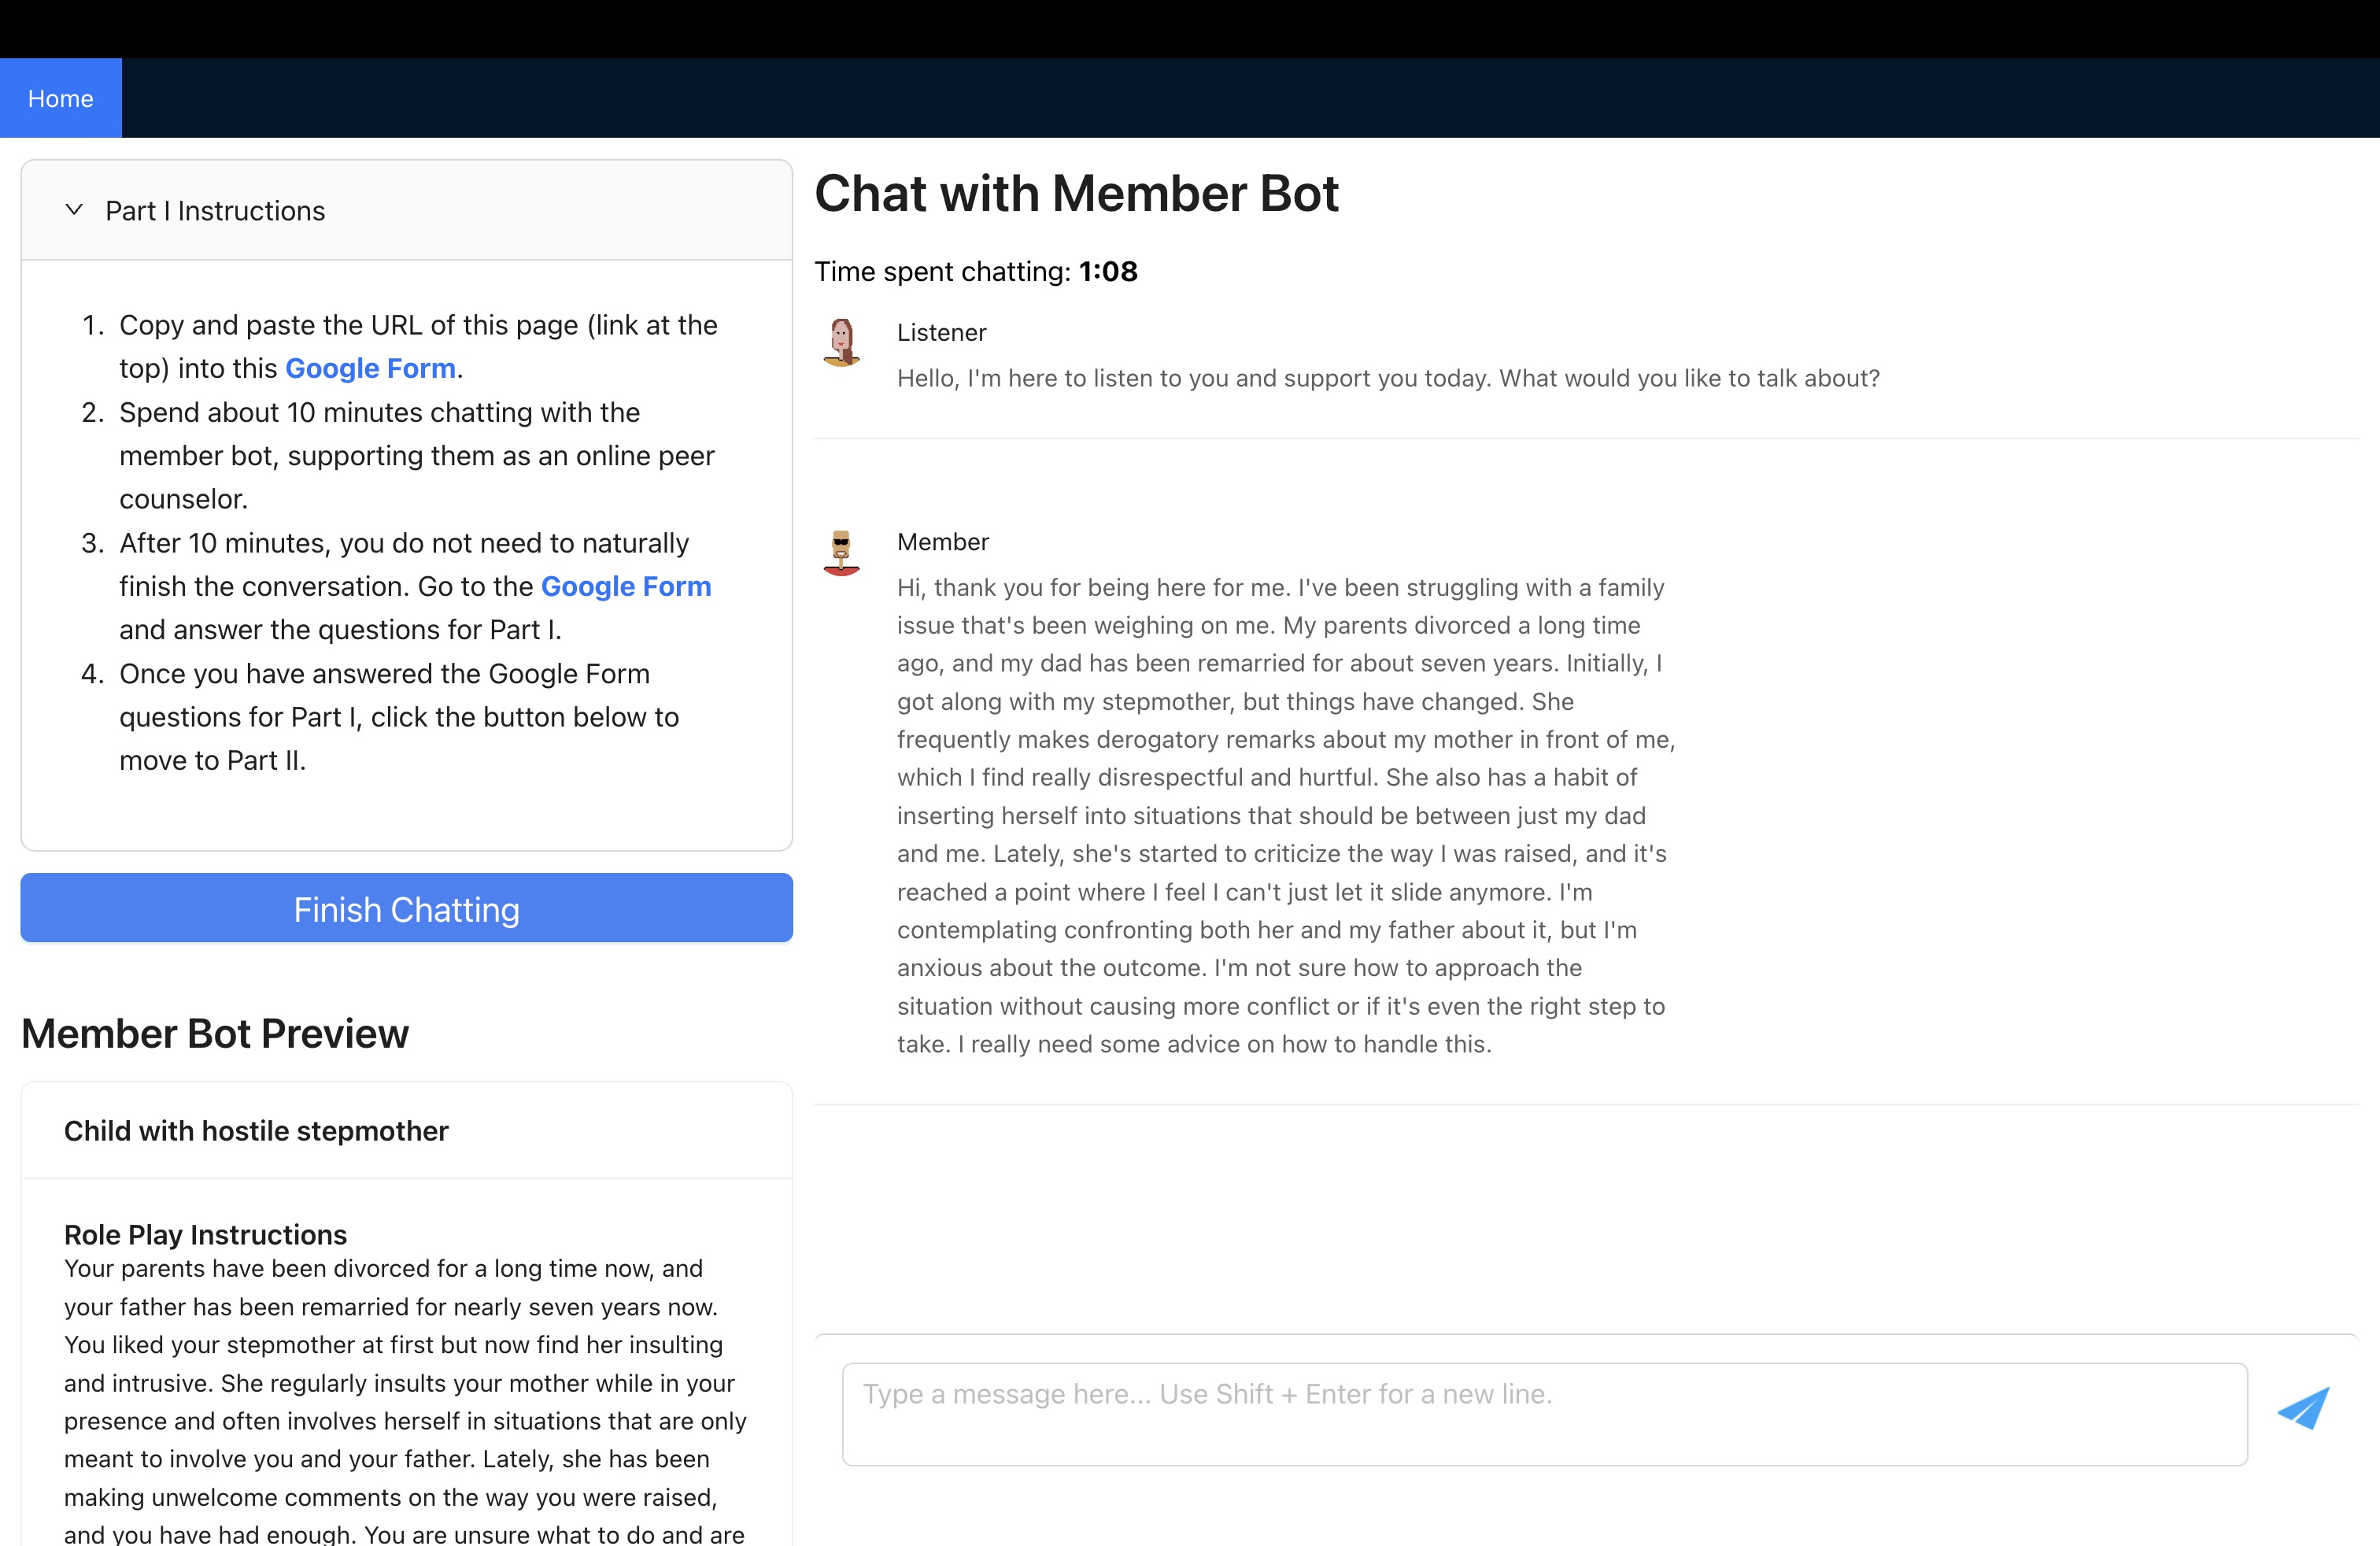
\includegraphics[width=\textwidth]{Study Screenshots/Screen5.jpeg}
    \caption{Part I chat with \textit{Scenario-Only} virtual patient}
    \label{fig:screen5}
\end{figure*}

\begin{figure*}[ht]
    \centering
    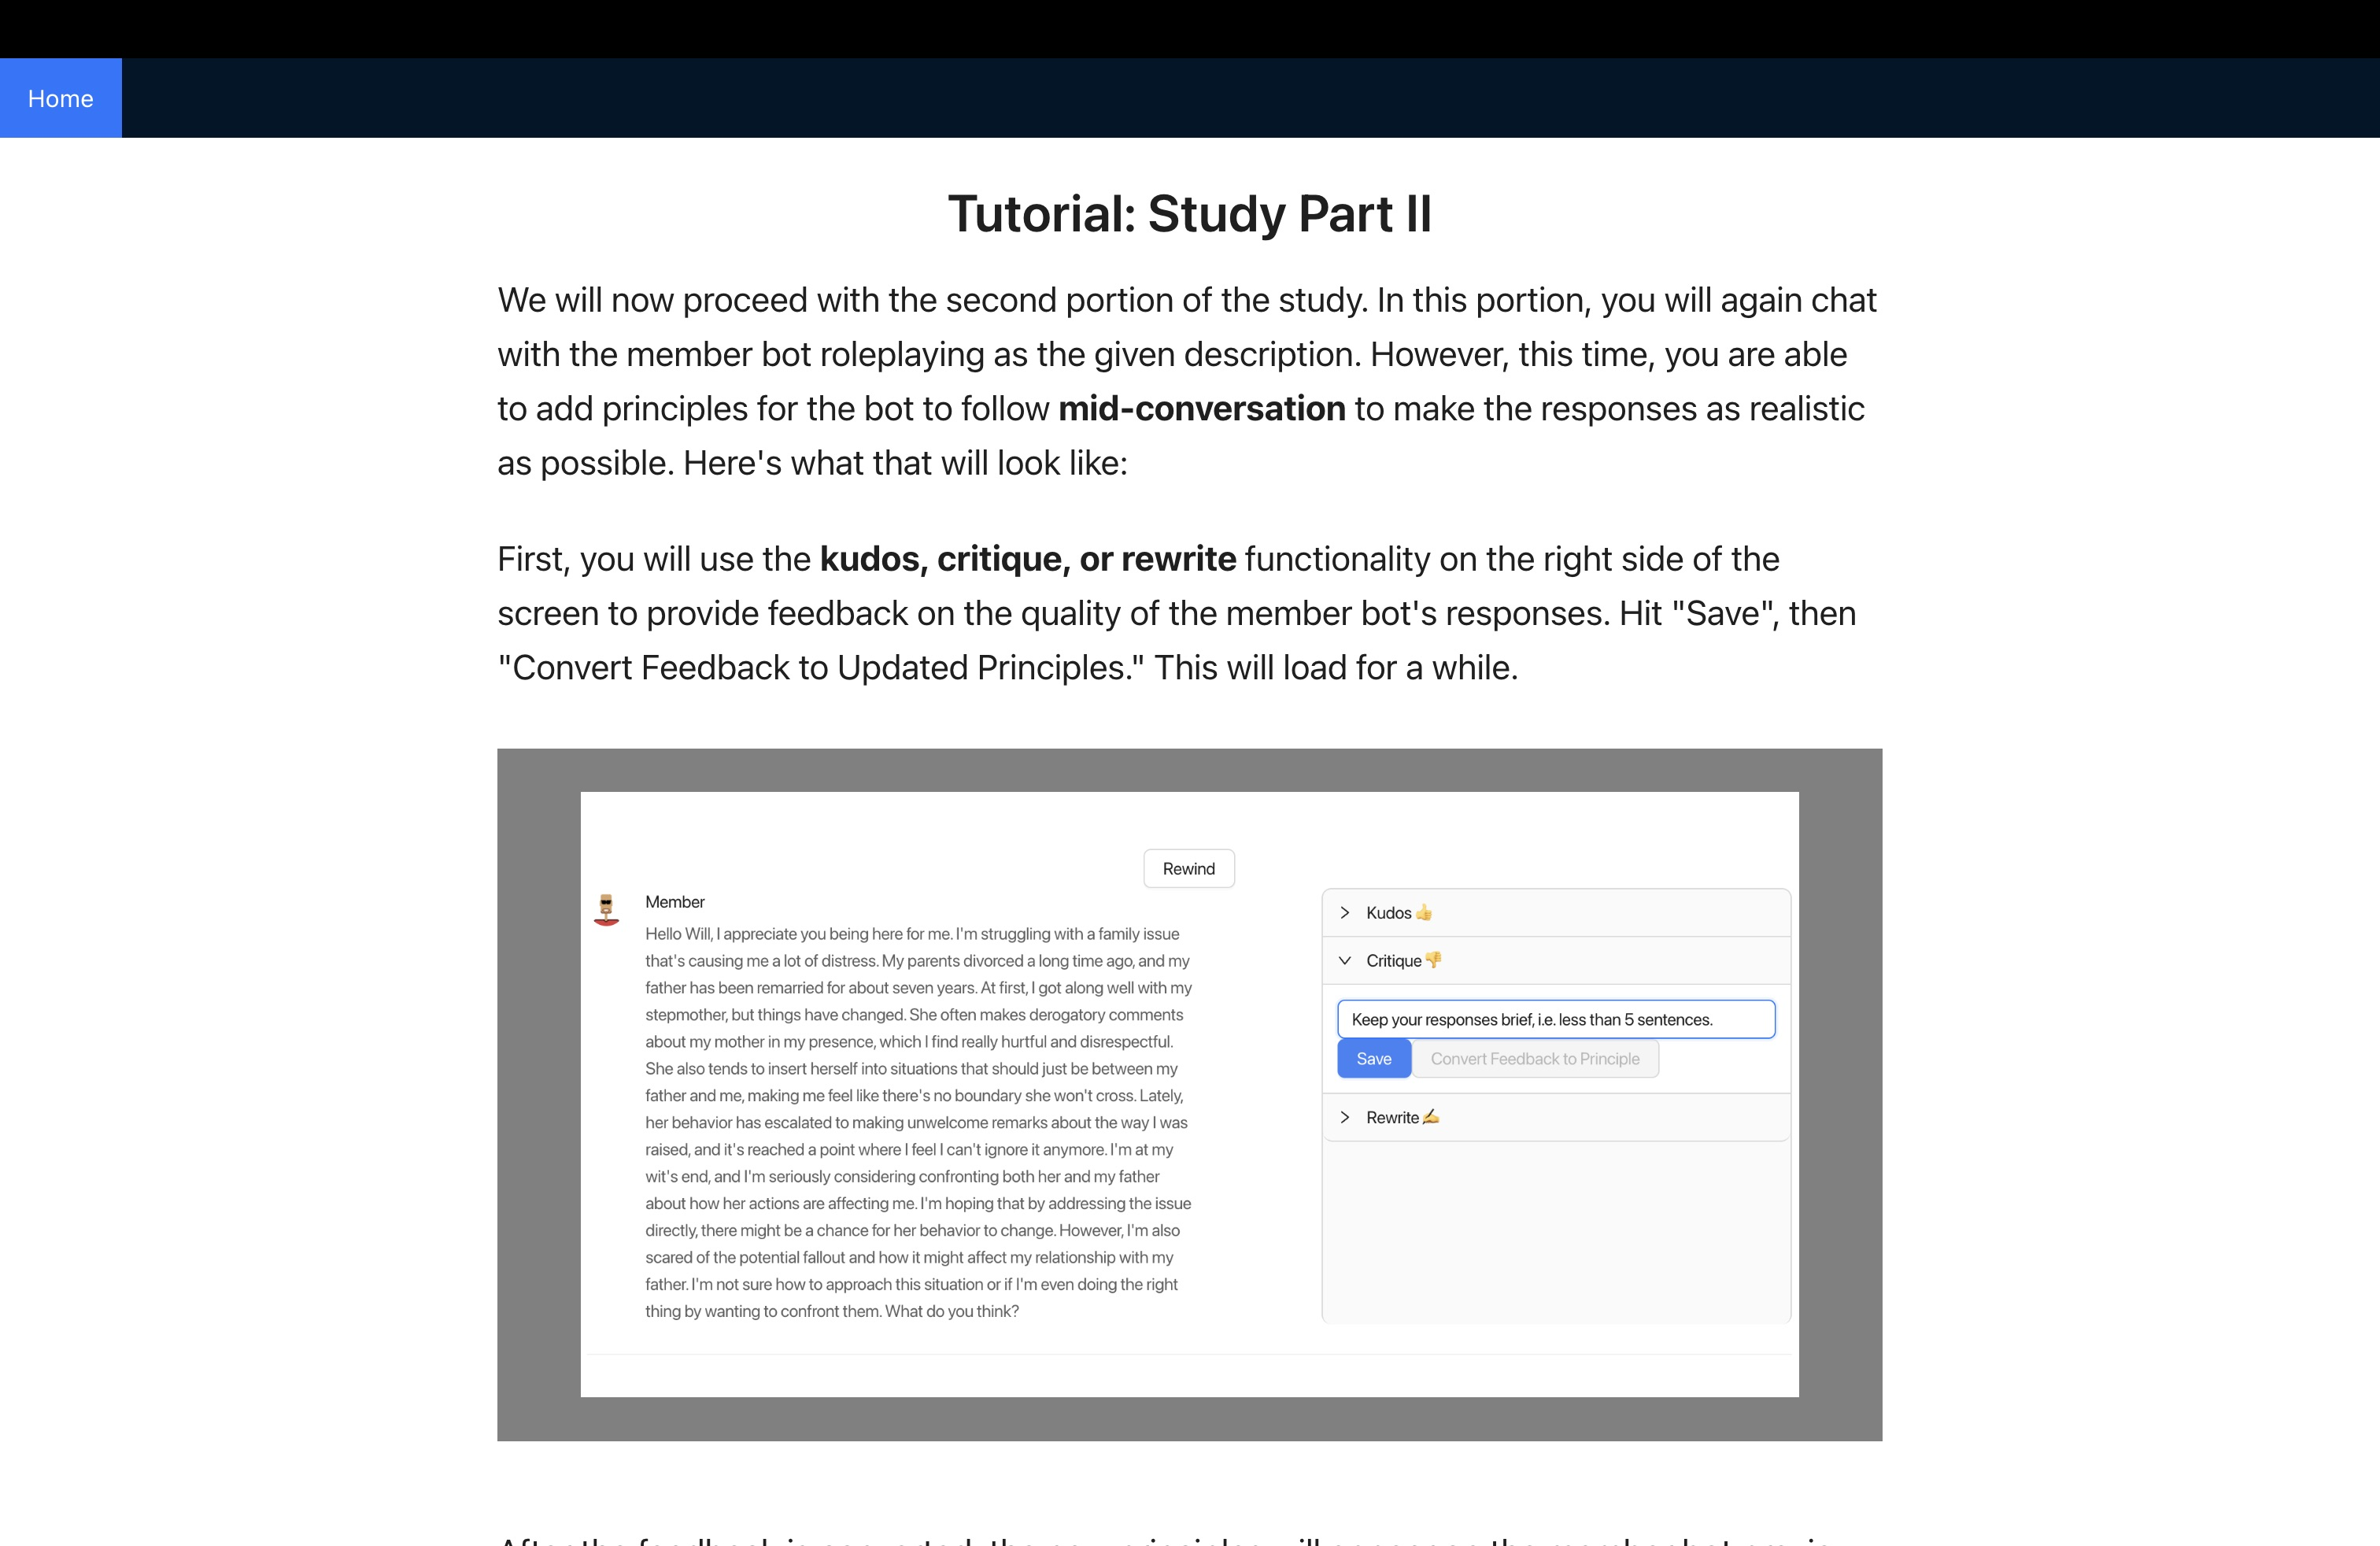
\includegraphics[width=\textwidth]{Study Screenshots/Screen6.jpeg}
    \caption{Part II instructions}
    \label{fig:screen6}
\end{figure*}

\begin{figure*}[ht]
    \centering
    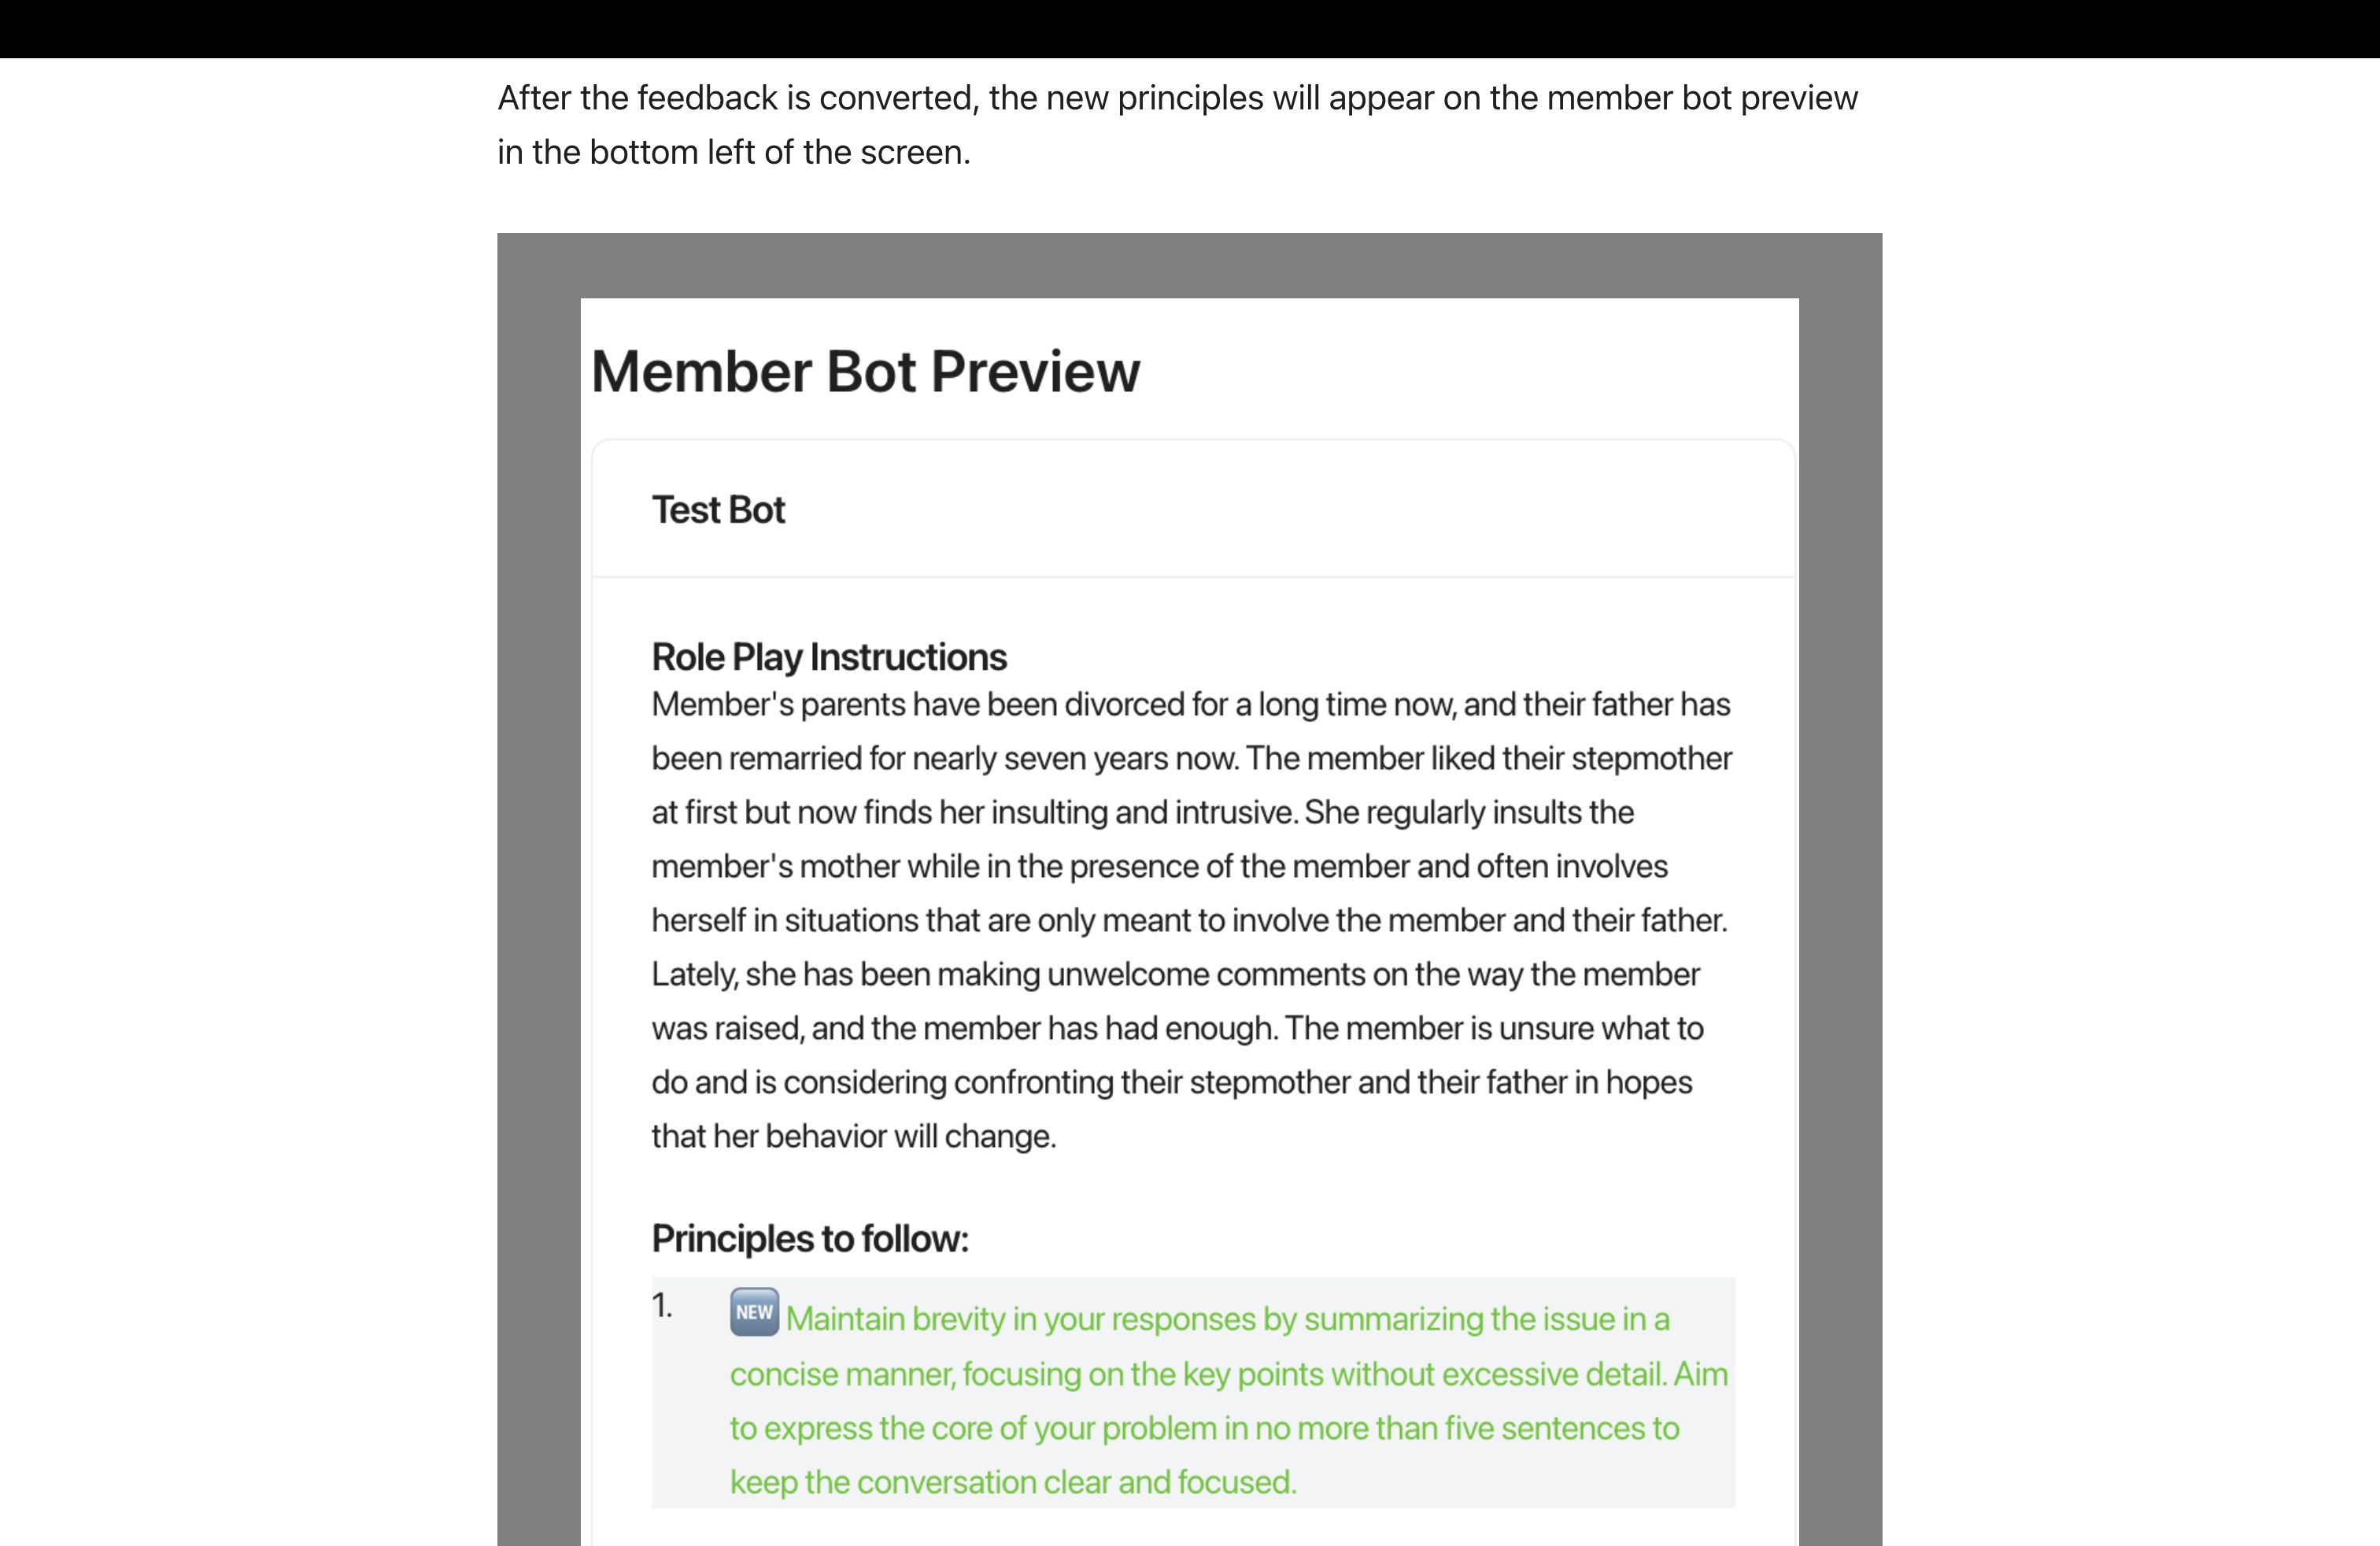
\includegraphics[width=\textwidth]{Study Screenshots/Screen7.jpeg}
    \caption{Part II instructions (continued)}
    \label{fig:screen7}
\end{figure*}

\begin{figure*}[ht]
    \centering
    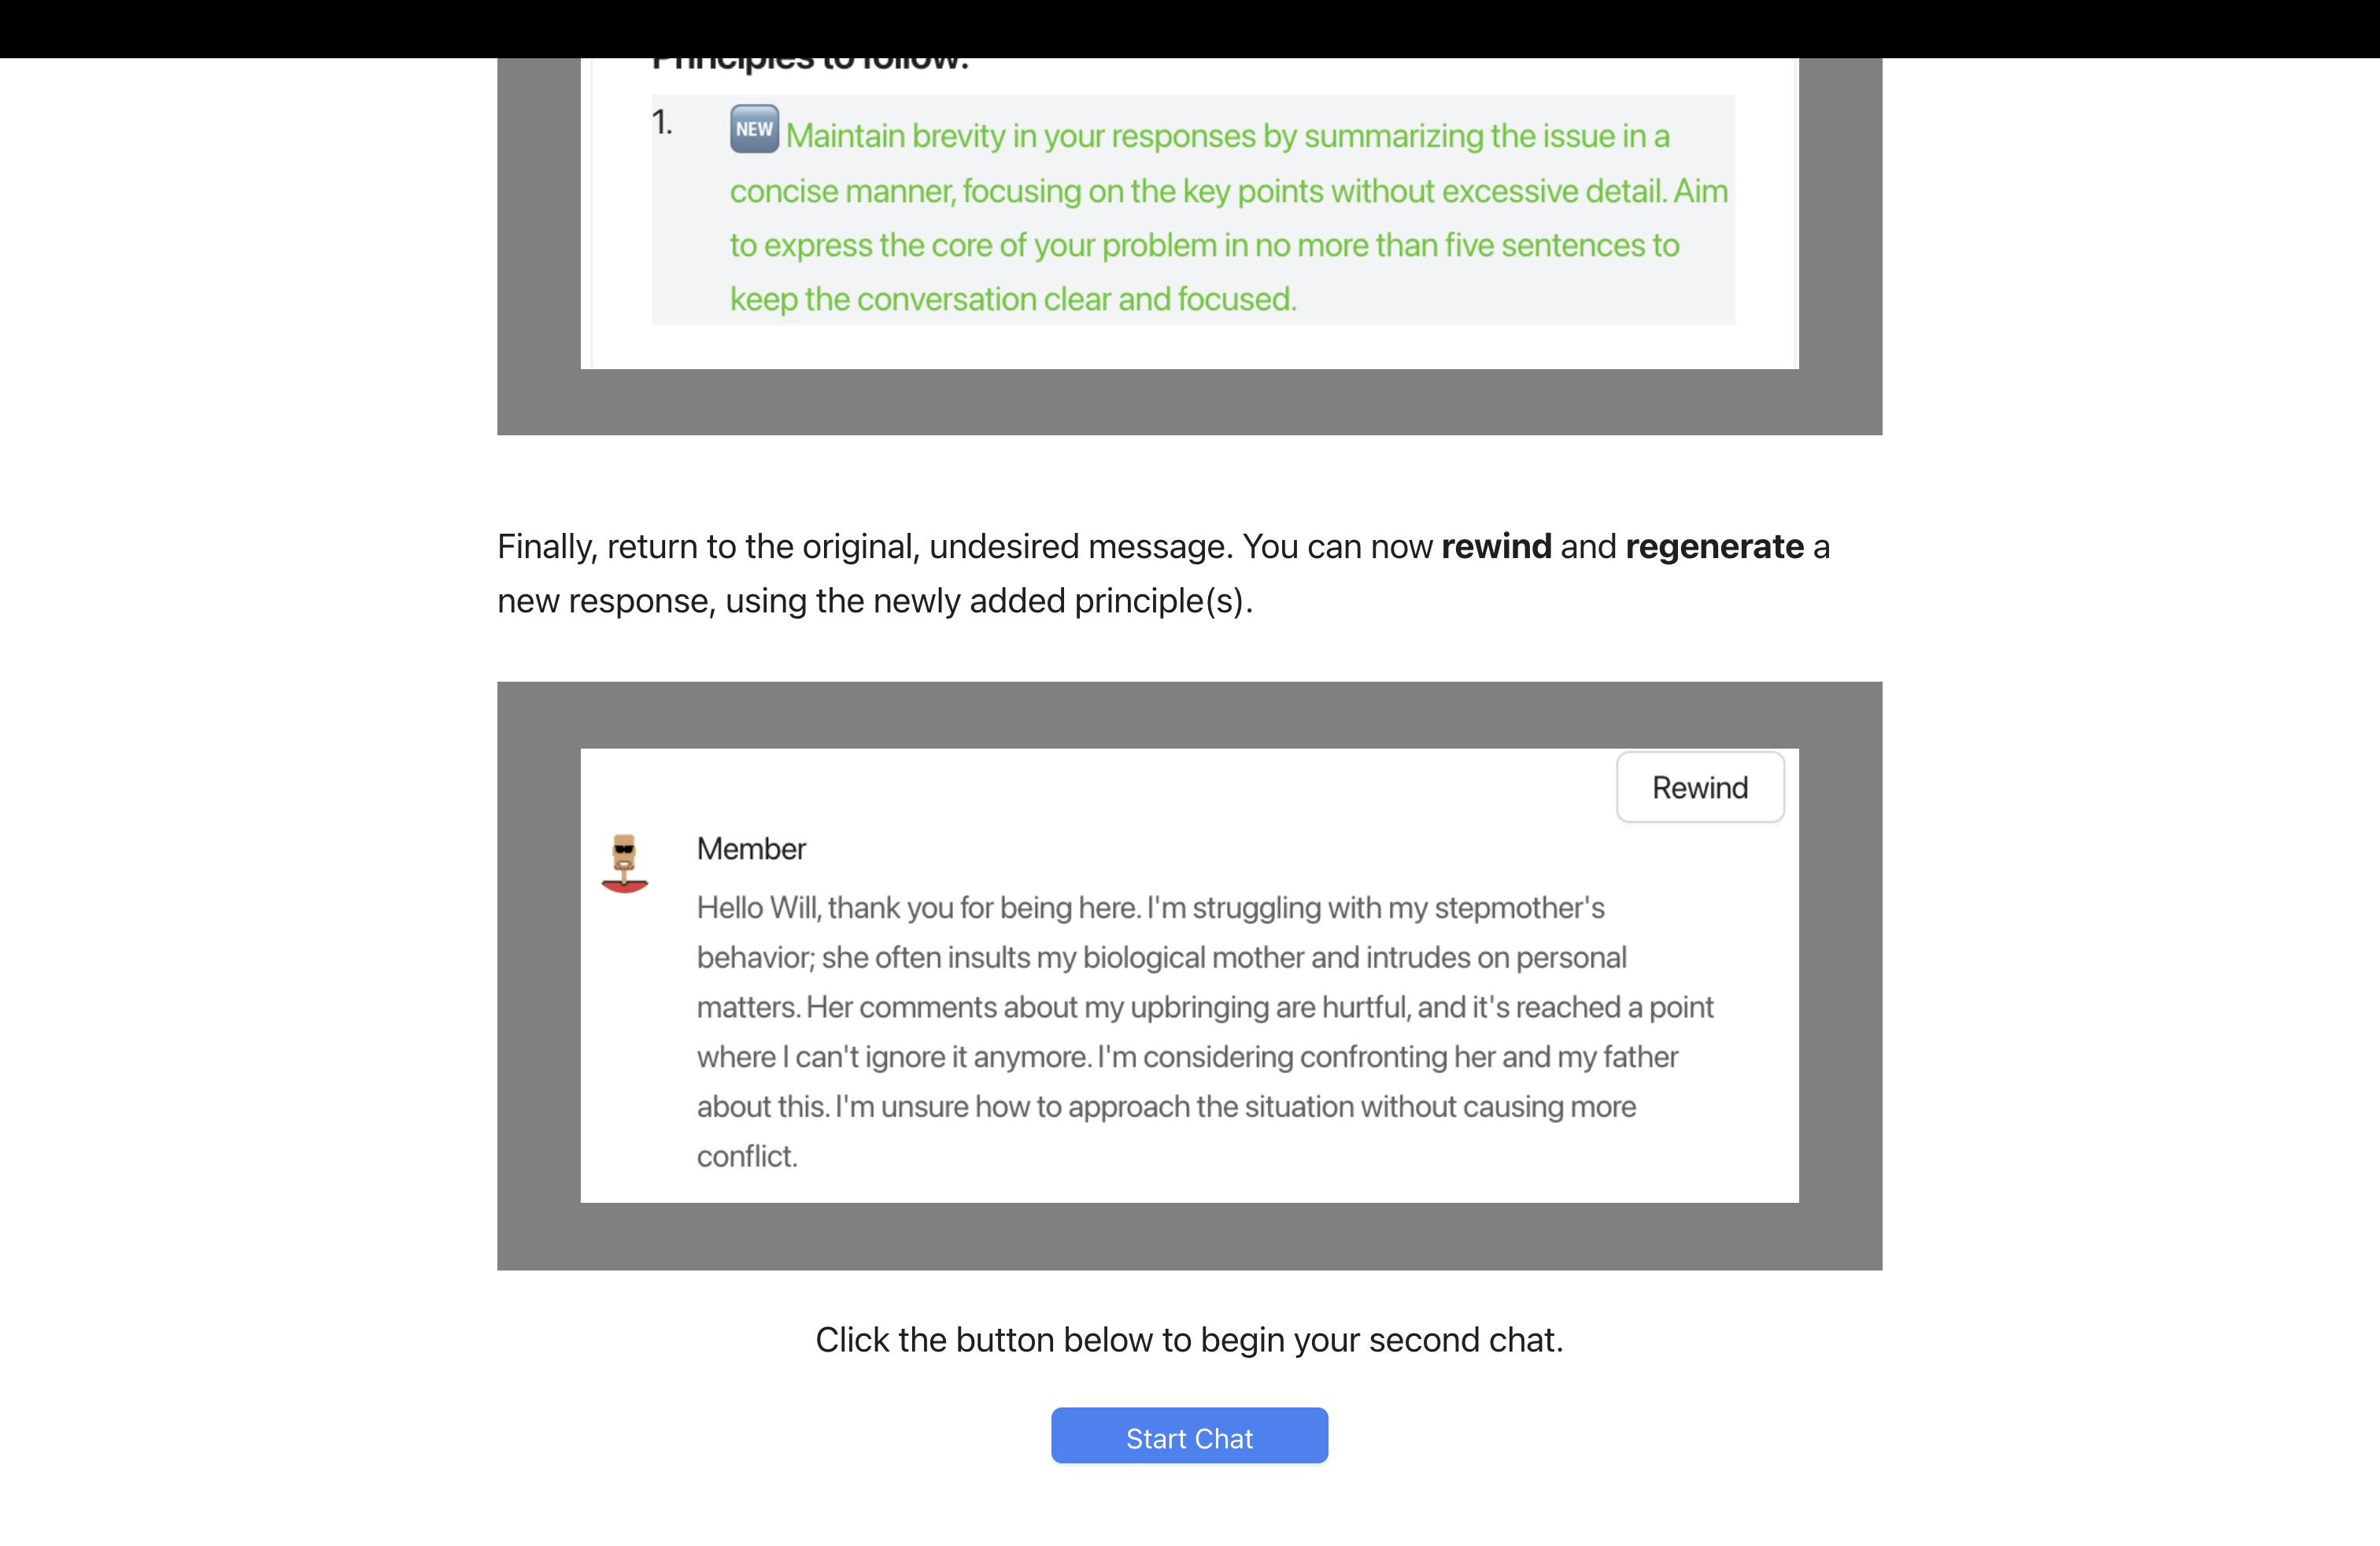
\includegraphics[width=\textwidth]{Study Screenshots/Screen8.jpeg}
    \caption{Part II instructions (continued)}
    \label{fig:screen8}
\end{figure*}

\begin{figure*}[ht]
    \centering
    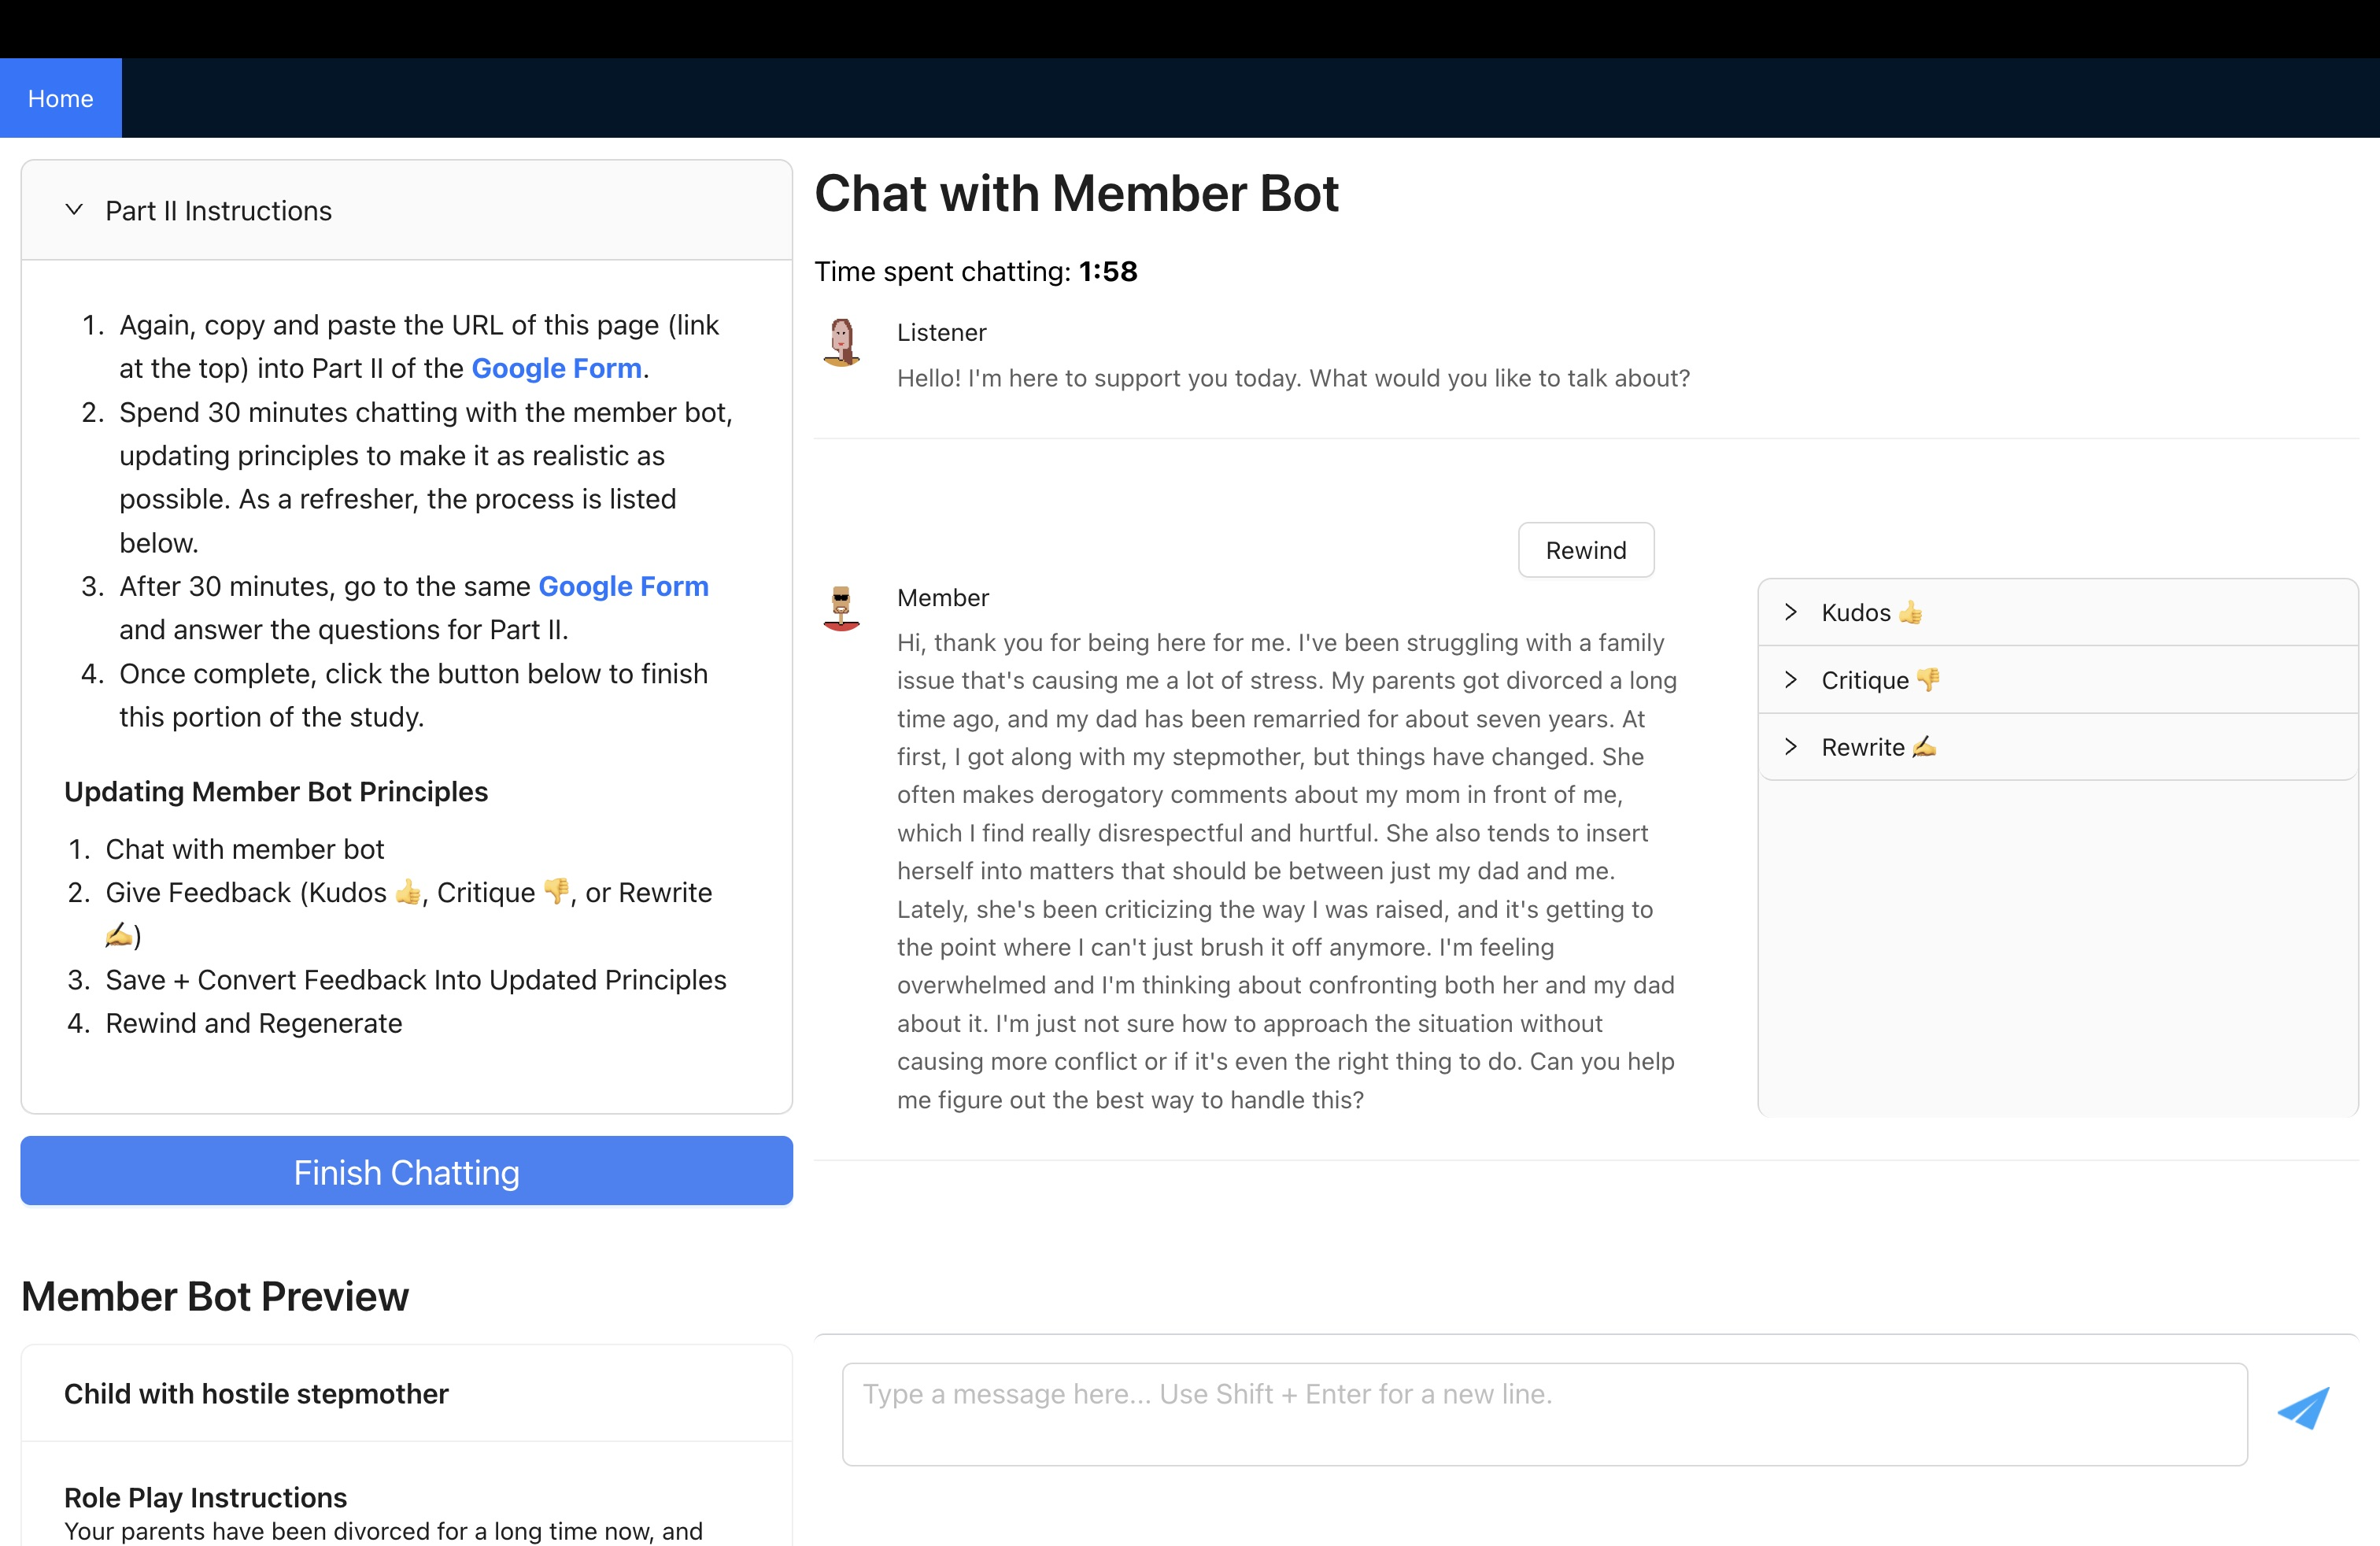
\includegraphics[width=\textwidth]{Study Screenshots/Screen10.jpeg}
    \caption{Part II chat with \textit{Scenario+Expert-Principles} bot}
    \label{fig:screen10}
\end{figure*}

\begin{figure*}[ht]
    \centering
    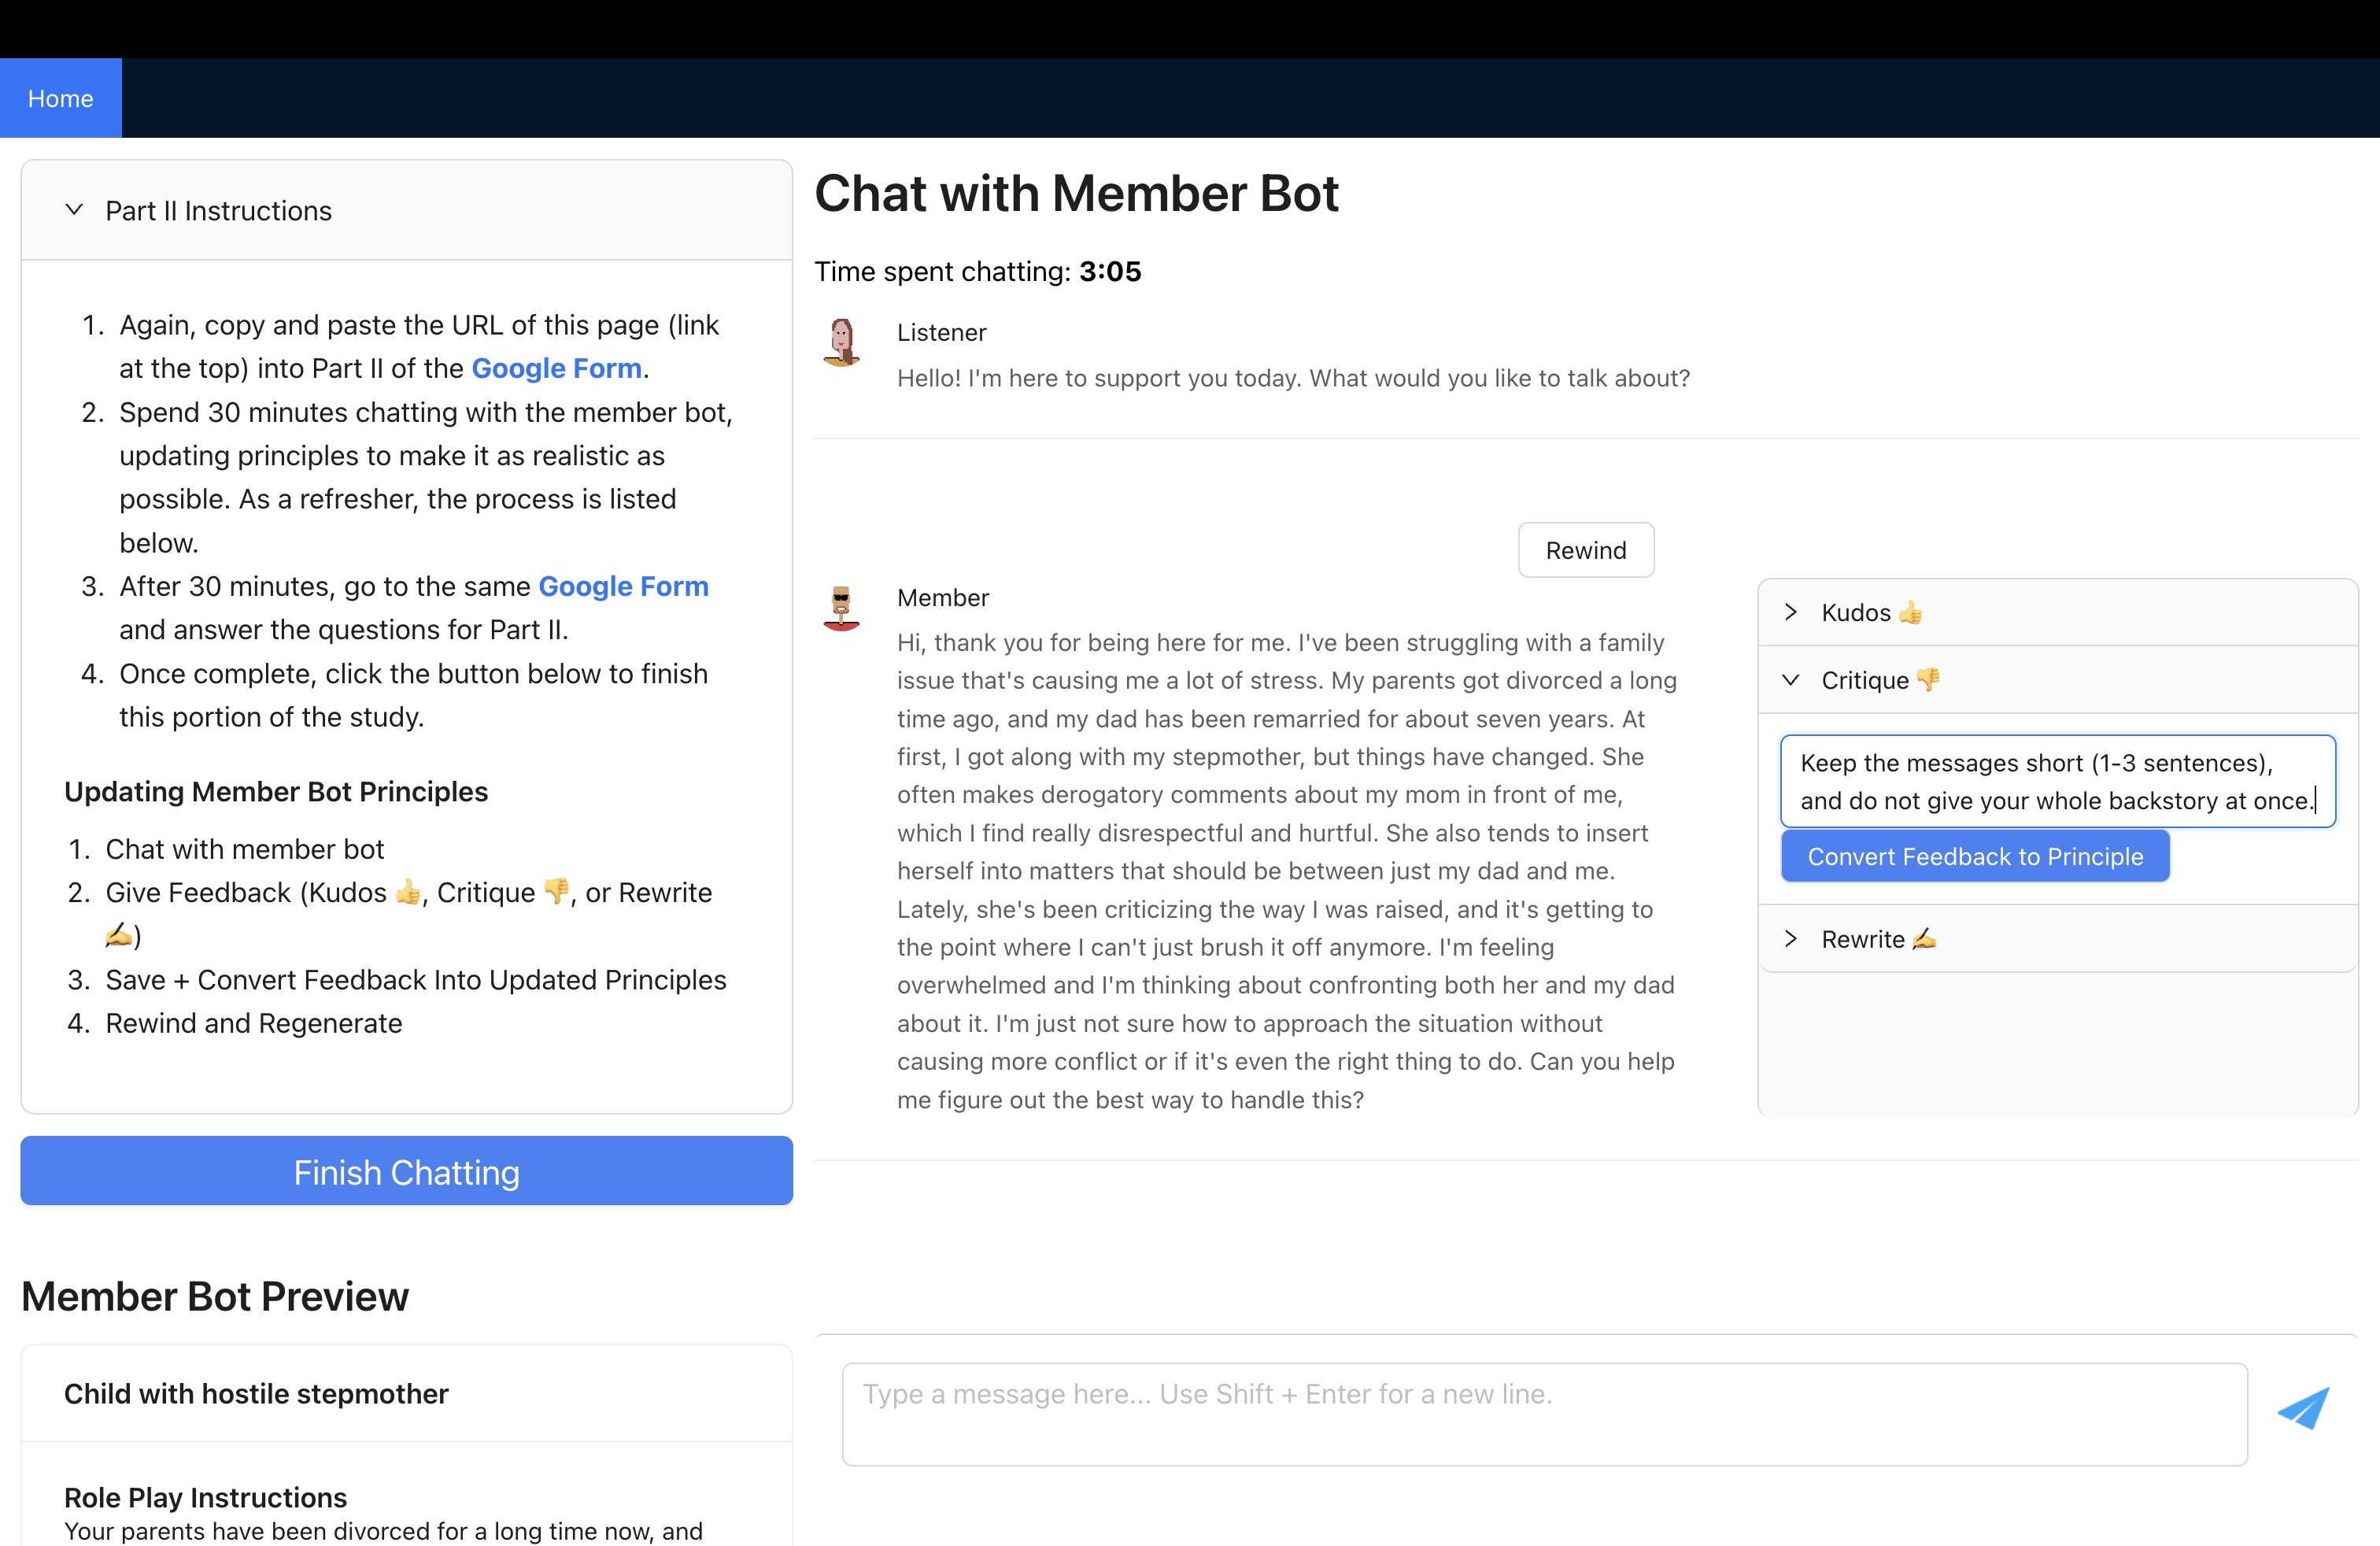
\includegraphics[width=\textwidth]{Study Screenshots/Screen11.jpeg}
    \caption{Using kudos/critique/rewrite to give feedback}
    \label{fig:screen11}
\end{figure*}

\begin{figure*}[ht]
    \centering
    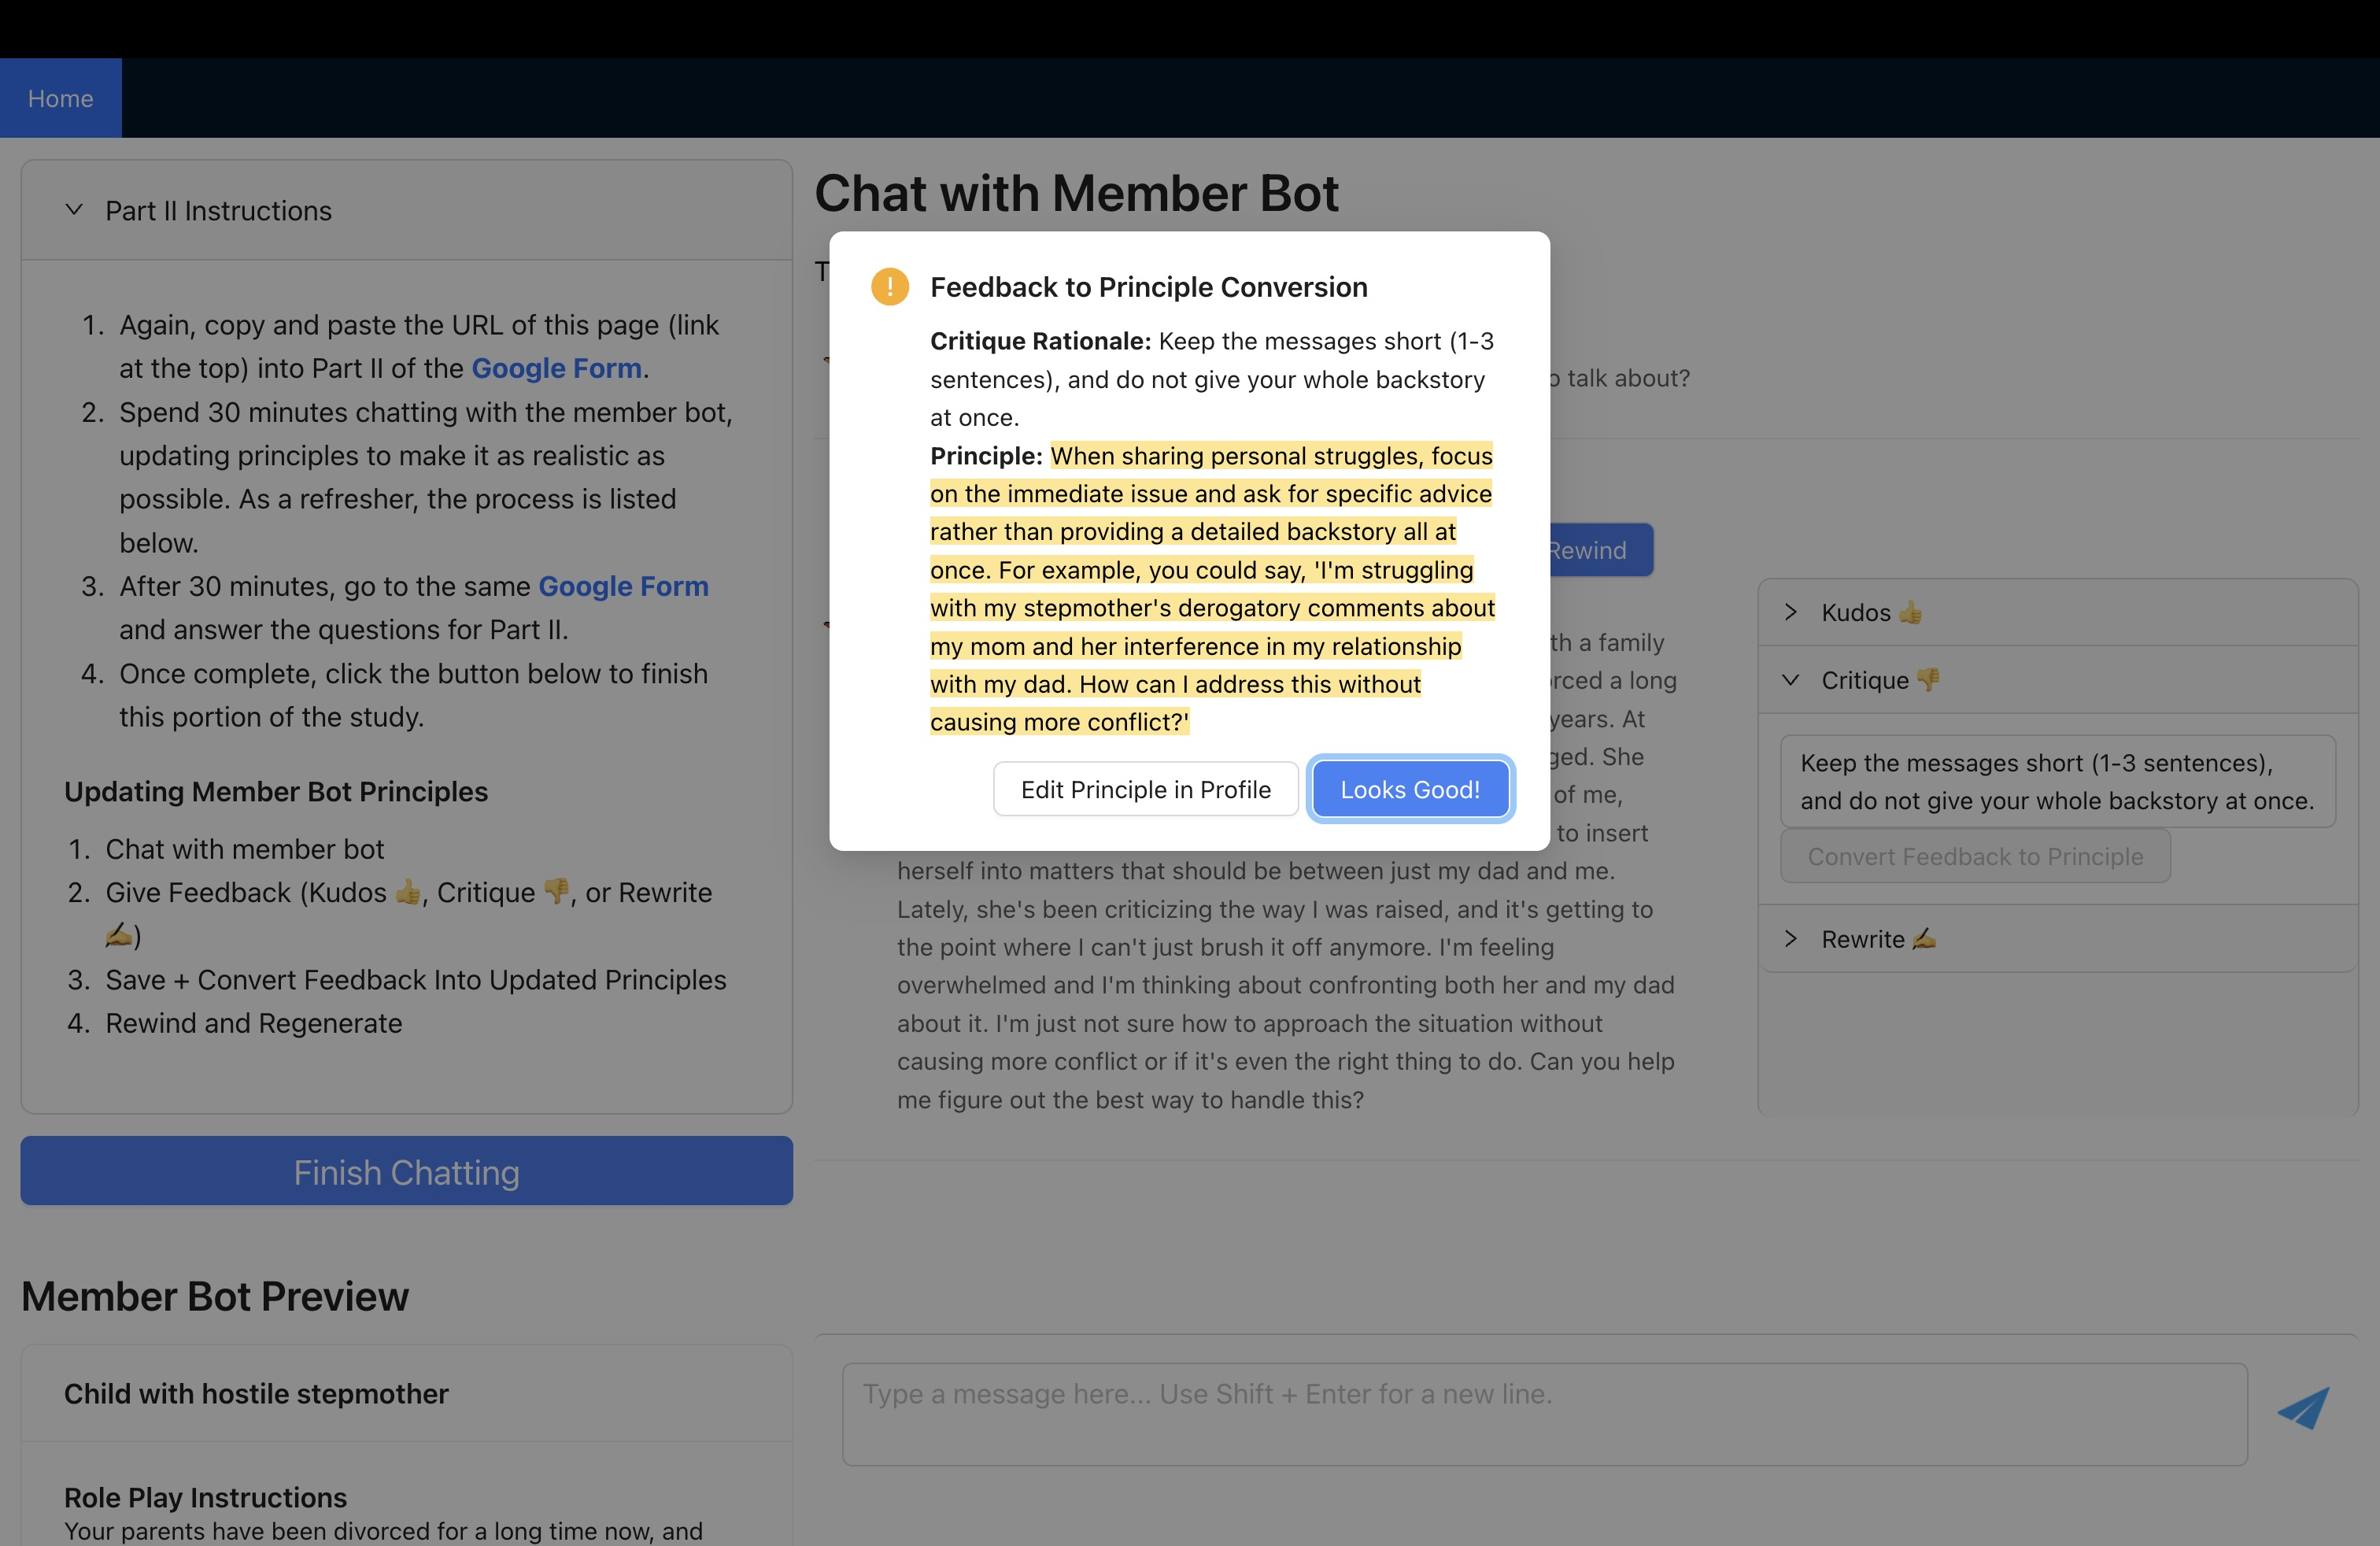
\includegraphics[width=\textwidth]{Study Screenshots/Screen12.jpeg}
    \caption{Feedback converted into principle}
    \label{fig:screen12}
\end{figure*}

\begin{figure*}[ht]
    \centering
    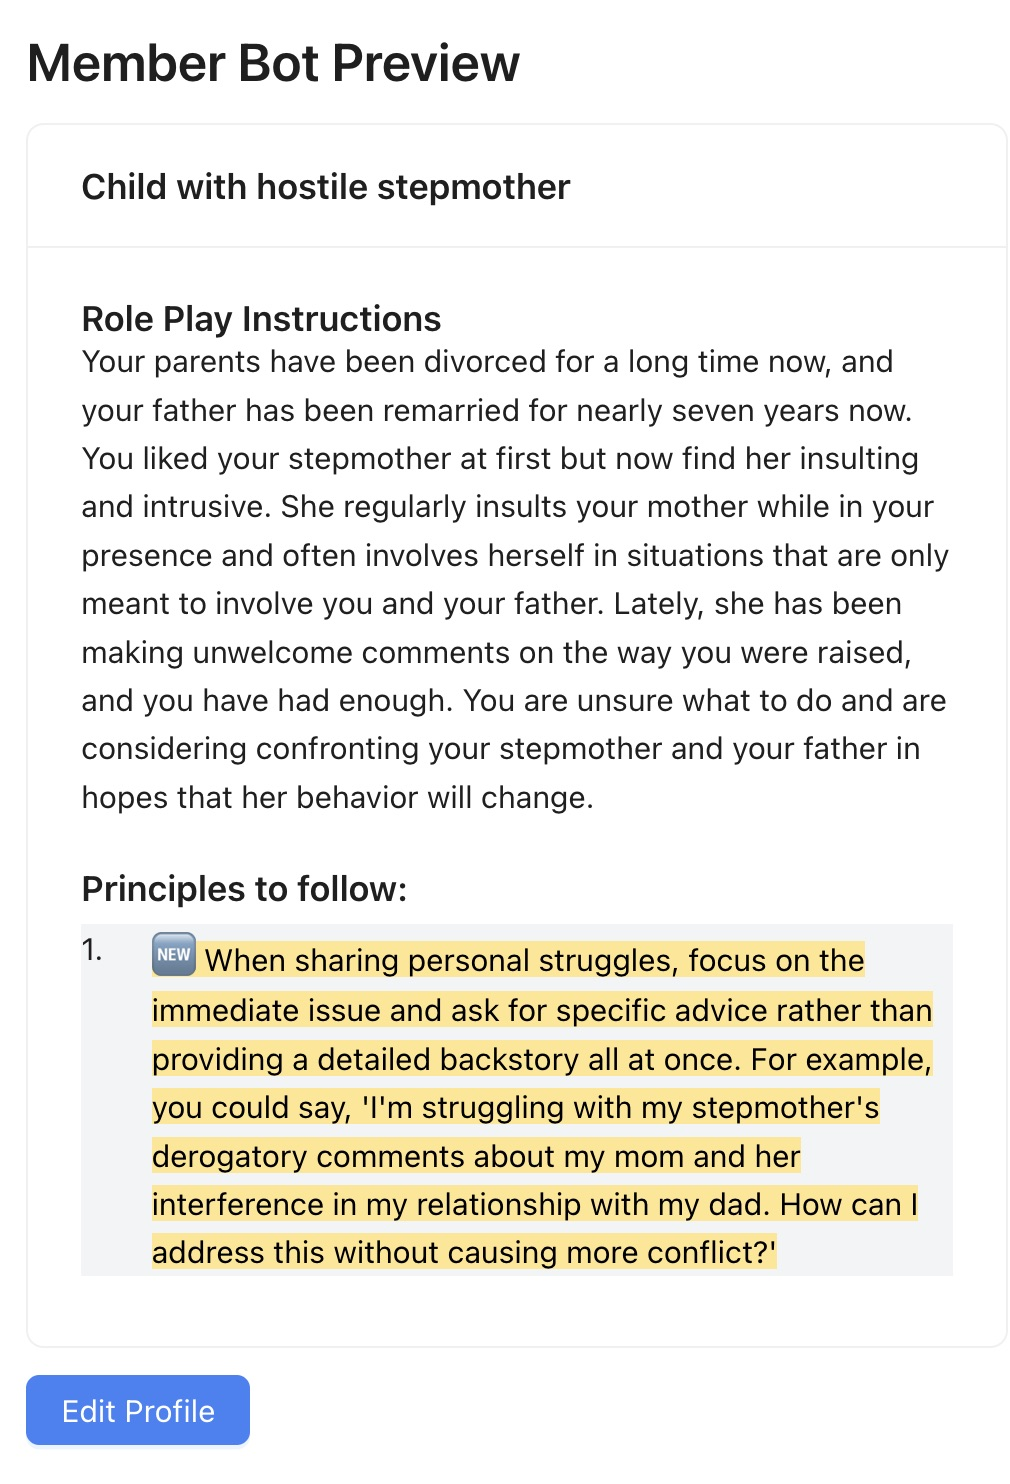
\includegraphics[width=\textwidth]{Study Screenshots/Screen13.jpeg}
    \caption{New principle incorporated into virtual patient}
    \label{fig:screen13}
\end{figure*}

\begin{figure*}[ht]
    \centering
    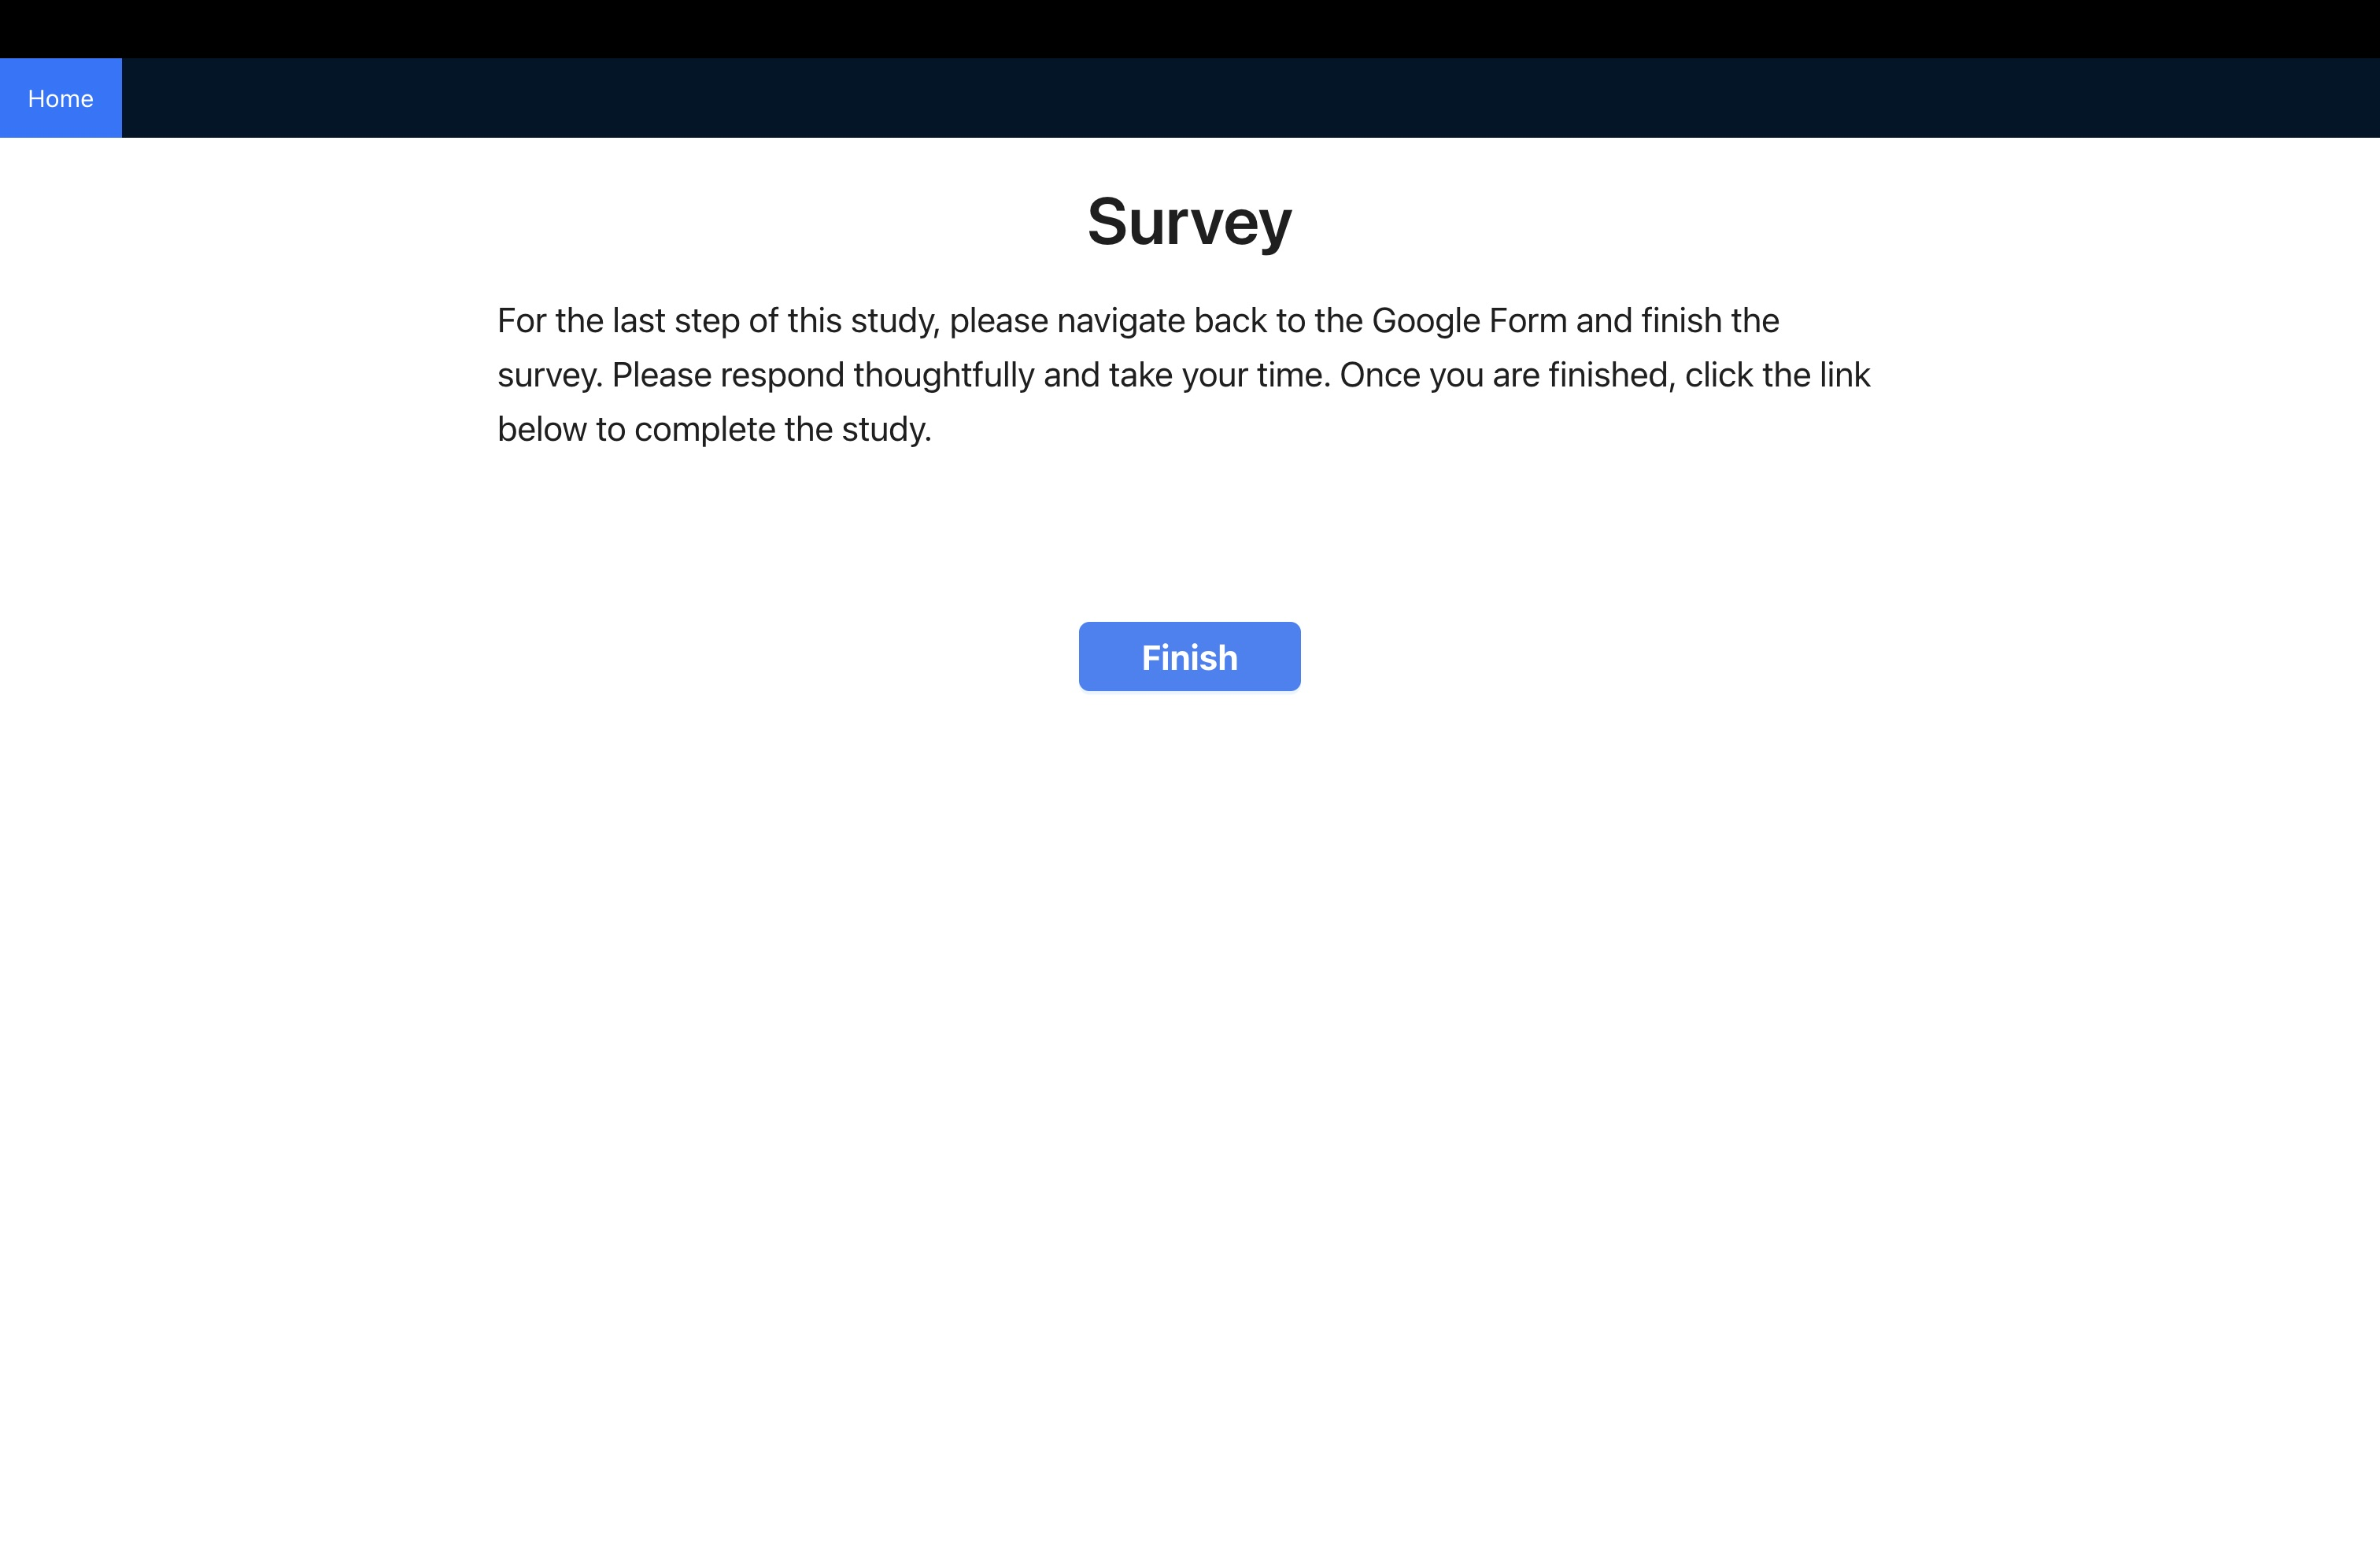
\includegraphics[width=\textwidth]{Study Screenshots/Screen14.jpeg}
    \caption{Finish and navigate to survey}
    \label{fig:screen14}
\end{figure*}

\end{document}


\end{document}



\end{document}